% =============================================================================
%  DỰ ÁN TỐT NGHIỆP — BÁO CÁO PHẦN 6
%  Đề tài: Thiết kế, Huấn luyện và Đánh giá Mô hình Dự báo Sản lượng Quang điện
%  Nhóm: The Outliers
%  Trường: Cao đẳng FPT Polytechnic — Chuyên ngành Phân tích Dữ liệu
%
%  ĐỊNH DẠNG: đồng bộ với Section2/3/4 (reports/Section{2,3,4}.tex) — cùng cỡ
%  chữ, cùng lề, cùng bảng màu khung code, cùng giãn dòng.
%  Khác biệt duy nhất: tài liệu này biên dịch bằng XeLaTeX (cần fontspec cho
%  tiếng Việt), nên dùng "TeX Gyre Heros" — bản Helvetica của TeX — thay cho
%  \usepackage[scaled]{helvet} của pdfLaTeX bên Section 2-3-4. Hình thức chữ
%  giống nhau; đổi engine trên tài liệu 238 KB nhiều hình sẽ vỡ build.
% =============================================================================

\documentclass[12pt,a4paper]{article}

% ======================== FONT & LỀ (khớp Section 2-3-4) =====================
\usepackage{fontspec}
\setmainfont{TeX Gyre Heros}   % = Helvetica sans-serif
\usepackage{geometry}
\geometry{top=2.5cm, bottom=2.5cm, left=3cm, right=2cm}

% ======================== GÓI CHUNG =========================================
\usepackage{amsmath,amssymb,amsfonts}
\usepackage{graphicx}
\usepackage{booktabs}
\usepackage{tabularx}
\usepackage{longtable}
\usepackage{array}
\usepackage{float}
\usepackage{caption}
\usepackage{subcaption}
\usepackage{xcolor}
\usepackage{listings}
\usepackage{microtype}
\usepackage[hyphens]{url}

% ======================== CẤU HÌNH CODE PYTHON (khớp Section 2-3-4) =========
\definecolor{codegreen}{rgb}{0,0.6,0}
\definecolor{codegray}{rgb}{0.5,0.5,0.5}
\definecolor{codepurple}{rgb}{0.58,0,0.82}
\definecolor{backcolour}{rgb}{0.96,0.96,0.94}
\definecolor{fptorange}{RGB}{245,130,32}

\lstdefinestyle{pythonstyle}{
    backgroundcolor   = \color{backcolour},
    commentstyle      = \color{codegreen},
    keywordstyle      = \color{magenta},
    numberstyle       = \tiny\color{codegray},
    stringstyle       = \color{codepurple},
    basicstyle        = \ttfamily\small,
    breakatwhitespace = false,
    breaklines        = true,
    captionpos        = r,
    keepspaces        = true,
    numbers           = left,
    numbersep         = 5pt,
    showspaces        = false,
    showstringspaces  = false,
    showtabs          = false,
    tabsize           = 4,
    frame             = single,
    rulecolor         = \color{codegray},
    linewidth         = \linewidth,
}
\lstset{style=pythonstyle}

% ======================== GIÃN DÒNG & THỤT ĐẦU DÒNG (khớp Section 2-3-4) ====
\usepackage{indentfirst}
\setlength{\parindent}{1cm}
\setlength{\parskip}{6pt}
\usepackage{setspace}
\onehalfspacing

% Nới chỗ ngắt dòng cho bảng rộng và URL dài của riêng báo cáo này
\emergencystretch=5em
\sloppy

% ======================== LIÊN KẾT ==========================================
\usepackage{hyperref}
\hypersetup{
    colorlinks  = true,
    breaklinks  = true,
    linkcolor   = black,
    citecolor   = blue,
    filecolor   = magenta,
    urlcolor    = blue,
    pdftitle    = {Bao cao Phan 6: Thiet ke, Huan luyen va Danh gia Mo hinh Du bao San luong Quang dien},
    pdfauthor   = {The Outliers - FPT Polytechnic},
    bookmarksnumbered = true,
}

\begin{document}

\begin{titlepage}
    \centering
    \vspace*{1cm}

    {\Huge \bfseries BÁO CÁO PHẦN 6 \par}
    \vspace{0.5cm}
    {\huge \bfseries THIẾT KẾ, HUẤN LUYỆN VÀ ĐÁNH GIÁ MÔ HÌNH DỰ BÁO SẢN LƯỢNG QUANG ĐIỆN \par}
    \vspace{0.3cm}
    {\large \bfseries BỔ SUNG CÁC KỸ THUẬT MÃ HÓA, CHUẨN HÓA \& CODE TỪ NOTEBOOKS \par}
    \vspace{0.2cm}
    {\large \itshape (Solar Forecasting Model Development \& Notebook Encoding Code Snippets) \par}
    
    \vspace{1.5cm}
    \textbf{Tác giả:} Nhóm Nghiên Cứu "The Outliers" --- Đồ Án Tốt Nghiệp \\
    \textbf{Đối tượng nghiên cứu:} Hệ thống dự báo sản lượng điện mặt trời cho 42 trạm quang điện độc lập \\
    \textbf{Tần suất dự báo:} 15 phút ($h=1$: 15m, $h=4$: 1h) \\
    \textbf{Trạng thái:} Báo cáo sử dụng bộ artifact v3 trong backup đầu tiên của workflow; số liệu dưới đây được truy xuất từ artifact, không chạy lại pipeline trong lượt cập nhật này.
    
    \vfill
    {\large TP. Hồ Chí Minh --- NĂM 2026 \par}
\end{titlepage}


\tableofcontents
\newpage

\section[TỔNG QUAN VÀ BỐI CẢNH NGHIỆP VỤ]{TỔNG QUAN VÀ BỐI CẢNH NGHIỆP VỤ\\(BUSINESS CONTEXT \& GOALS)}

Điện mặt trời là nguồn năng lượng tái tạo có tính \textbf{biến động cao (intermittent)} và phụ thuộc chặt chẽ vào các điều kiện khí tượng như bức xạ mặt trời toàn phần ($GHI$), bức xạ trực tiếp ($DNI$), độ mây phủ ($cloud\_cover$) và nhiệt độ môi trường. Trong thực tế ngành điện, việc dự báo sản lượng quang điện với tần suất 15 phút không chỉ là một bài toán kỹ thuật dữ liệu (Data Science), mà mang \textbf{ý nghĩa nghiệp vụ tài chính và vận hành hạ tầng lưới điện cực kỳ quan trọng}.

\subsection{Ý nghĩa nghiệp vụ đối với Trung tâm Điều độ Hệ thống Điện (A0 / NSMO)}
\begin{enumerate}
    \item \textbf{Lập lịch phát điện tối ưu (Unit Commitment \& Economic Dispatch):} Dự báo chính xác sản lượng điện mặt trời theo từng block 15 phút giúp đơn vị điều độ chủ động điều tiết các nguồn điện truyền thống (thủy điện tích năng, tua-bin khí), giảm chi phí duy trì công suất quay dự phòng (\textit{Spinning Reserve Cost}).
    \item \textbf{Đảm bảo an toàn tần số và điện áp lưới (Grid Frequency \& Voltage Stability):} Việc điện mặt trời sụt giảm chớp nhoáng do hiện tượng mây phủ (\textit{Cloud Transient Event}) nếu không được dự báo trước sẽ gây ra biến động tần số, cơ nguy quá tải cục bộ trên đường dây truyền tải.
\end{enumerate}

\subsection{Ý nghĩa nghiệp vụ đối với Chủ đầu tư trang trại quang điện}
\begin{enumerate}
    \item \textbf{Tối ưu hóa doanh thu \& Giảm chi phí phạt trệch cân bằng (Imbalance Settlement Penalties):} Theo quy định thị trường điện, các nhà máy điện mặt trời phải nộp bản tin dự báo công suất phát trước mỗi chu kỳ giao dịch. Dự báo sai lệch vượt quá ngưỡng cho phép sẽ chịu mức phí phạt trệch cân bằng công suất rất nặng.
    \item \textbf{Giám sát sức khỏe vật lý tài sản (Performance Ratio - PR \& Capacity Factor - F):} Mô hình dự báo đóng vai trò là "mức cơ sở lý thuyết chuẩn" để đối chiếu với sản lượng thực đo. Nếu sản lượng thực tế thấp hơn hẳn dự báo trong điều kiện bức xạ cao, mô hình giúp phát hiện sớm hiện tượng suy giảm hiệu suất tấm pin (\textit{Panel Degradation}), quá nhiệt Inverter hoặc bám bẩn bề mặt (\textit{Soiling Loss}).
\end{enumerate}


\subsection{Danh Mục Thuật Ngữ \& Từ Viết Tắt Khoa Học (Glossary of Terms \& Acronyms)}
Để bảo đảm tính rõ ràng, minh bạch và dễ tra cứu cho Hội đồng Đánh giá Đồ án, Bảng \ref{tab:glossary} giải thích chi tiết ý nghĩa kỹ thuật, công thức và chuẩn quốc tế của toàn bộ các từ viết tắt được sử dụng trong báo cáo:

\begin{table}[H]
\centering
\caption{Bảng Tra Cứu Chi Tiết Các Thuật Ngữ Kỹ Thuật \& Từ Viết Tắt Khoa Học trong Báo Cáo}
\label{tab:glossary}
\scriptsize
\begin{tabularx}{\linewidth}{|l|l|X|}
\hline
\textbf{Ký Hiệu} & \textbf{Tên Gốc / Tiếng Anh} & \textbf{Giải Thích Ý Nghĩa Kỹ Thuật \& Chuẩn Quốc Tế} \\ \hline
\textbf{ST} & Standard Test Conditions & \textbf{Điều kiện Thử nghiệm Tiêu chuẩn} cho tấm pin mặt trời theo chuẩn quốc tế \textbf{IEC 60904-3}~\cite{iec60904} (gồm: Bức xạ $1000 \text{ W/m}^2$, Nhiệt độ cell pin $25^\circ\text{}$, và Khối không khí $\text{AM} = 1.5$). $P_{\text{stc}}$ là công suất định mức ($\text{kWp}$) do nhà sản xuất chứng nhận ở ST. \\ \hline
\textbf{GHI} & Global Horizontal Irradiance & \textbf{Tổng Bức xạ Mặt trời trên Mặt phẳng Ngang} ($\text{W/m}^2$), gồm tổng của Bức xạ Trực tiếp ($DNI$) và Bức xạ Khuếch tán ($DHI$). \\ \hline
\textbf{DNI} & Direct Normal Irradiance & \textbf{Bức xạ Trực tiếp Vuông góc} với tia nắng mặt trời ($\text{W/m}^2$), chiếu thẳng từ đĩa mặt trời khi không bị mây che. \\ \hline
\textbf{DHI} & Diffuse Horizontal Irradiance & \textbf{Bức xạ Khuếch tán Bầu trời} trên mặt phẳng ngang ($\text{W/m}^2$), tạo ra do ánh sáng mặt trời bị tán xạ bởi mây, bụi và khí quyển. \\ \hline
\textbf{POA} & Plane of Array Irradiance & \textbf{Bức xạ trên Mặt phẳng Nghiêng Dàn Pin} ($\text{W/m}^2$), là tổng bức xạ thực tế chiếu lên bề mặt tấm pin lắp nghiêng. \\ \hline
\textbf{PR} & Performance Ratio & \textbf{Tỷ số Hiệu suất Hệ thống} (\%), đo tỷ lệ giữa năng lượng phát ra thực tế so với năng lượng lý thuyết thu nhận ở điều kiện bức xạ $POA$. \\ \hline
\textbf{F} & Capacity Factor & \textbf{Hệ số Sử dụng Công suất} (\%), tỷ lệ giữa sản lượng phát thực tế trong ngày so với sản lượng tối đa nếu phát liên tục ở $P_{\text{stc}}$ trong 24h. \\ \hline
\textbf{GMM} & Gaussian Mixture Model & \textbf{Mô hình Hỗn hợp Gauss}: Thuật toán học máy thống kê biểu diễn phân bố dữ liệu bằng tổng các hàm mật độ Gauss, dùng để tính mật độ xác suất (density) $p_{\text{gmm}} < \theta$ lọc Outlier cục bộ. \\ \hline
\textbf{IF / iForest} & Isolation Forest & \textbf{Rừng Cô lập}~\cite{liu2008if}: Thuật toán phân lập điểm bất thường dựa trên cấu trúc cây phân tách ngẫu nhiên. Đường đi cô lập ngắn tương ứng với điểm bất thường cao; pipeline hiện tại dùng \texttt{contamination}=0.03 để tạo cờ IF, không dùng ngưỡng score cố định $0.65$. \\ \hline
\textbf{VIF} & Variance Inflation Factor & \textbf{Hệ số Phóng đại Phương sai}: Chỉ số đo lường mức độ đa cộng tuyến giữa các đặc trưng đầu vào. $VIF > 10$ cho thấy đặc trưng bị trùng lặp thông tin nghiêm trọng. \\ \hline
\textbf{SHAP} & SHapley Additive exPlanations & Phương pháp giải thích mô hình AI dựa trên \textbf{Lý thuyết Trò chơi Hợp tác (Cooperative Game Theory)} của Giáo sư Lloyd Shapley (Nobel Kinh tế 2012), đo lường mức đóng góp biên trị giá $\phi_i$ cho từng dự báo. \\ \hline
\textbf{XAI} & eXplainable Artificial Intelligence & \textbf{Trí tuệ Nhân tạo Có thể Giải thích}: Tập hợp các phương pháp kỹ thuật (như SHAP, Feature Importance) giúp mở "hộp đen AI" để kỹ sư hiểu rõ cơ chế dự báo. \\ \hline
\textbf{WAPE} & Weighted Absolute Percentage Error & \textbf{Sai số Phần trăm Tuyệt đối Có Trọng số} (\%), chỉ số đánh giá sai số chính của bài toán năng lượng, bằng tổng độ lệch tuyệt đối chia cho tổng sản lượng thực tế. \\ \hline
\textbf{MAE} & Mean Absolute Error & \textbf{Sai số Tuyệt đối Trung bình} ($\text{kWh}$), đo khoảng cách trung bình giữa thực tế và dự báo. \\ \hline
\textbf{RMSE} & Root Mean Squared Error & \textbf{Căn bậc hai Sai số Bình phương Trung bình} ($\text{kWh}$), chỉ số phạt nặng các điểm dự báo lệch lớn. \\ \hline
\textbf{pvlib} & PV Modeling Library & Thư viện vật lý mô hình hóa hệ thống quang điện chuẩn quốc tế phát triển bởi \textbf{Phòng Thí nghiệm Quốc gia Sandia (Sandia National Laboratories, Bộ Năng lượng Mỹ)}. \\ \hline
\textbf{Optuna} & Hyperparameter Optimization Framework~\cite{optuna2019} & Thư viện tự động tối ưu hóa siêu tham số mô hình dựa trên thuật toán \textbf{Bayesian Optimization TPE (Tree-structured Parzen Estimator)}. \\ \hline
\end{tabularx}
\end{table}



\section{Cơ sở Lý thuyết}
\label{chap:lythuyet}

\subsection{Tổng quan về Năng lượng mặt trời và Bức xạ quang điện}
\label{sec:solar_theory}

Hệ thống quang điện (PV) chuyển đổi năng lượng bức xạ mặt trời trực tiếp thành điện năng thông qua hiệu ứng quang điện trong chất bán dẫn. Hiệu suất chuyển đổi và khả năng vận hành của hệ thống phụ thuộc chặt chẽ vào các chỉ số lý thuyết sau:
\begin{itemize}
    \item \textbf{Performance Ratio (PR):} Tỷ lệ đánh giá hiệu suất nguồn lưới, được xác định bằng tỷ số giữa sản lượng điện thực tế tạo ra và sản lượng lý thuyết trong điều kiện bức xạ lý tưởng. PR phản ánh mức độ tổn hao năng lượng do nhiệt độ, bụi bẩn và hiệu suất của bộ biến đổi (Inverter).
    \item \textbf{Capacity Factor (F):} Hệ số công suất, được tính bằng tỷ lệ giữa sản lượng điện thực tế thu được trong một khoảng thời gian so với sản lượng điện tối đa mà trạm có thể phát nếu vận hành liên tục ở công suất thiết kế cực đại.
    \item \textbf{Specific Yield:} Sản lượng điện đặc trưng, biểu thị lượng điện năng tạo ra trên mỗi đơn vị công suất đỉnh lắp đặt (đo bằng đơn vị kWh/kWp), hỗ trợ so sánh hiệu suất giữa các trạm có quy mô khác nhau.
\end{itemize}

\subsection{Kiến trúc Kho dữ liệu đa chiều (Data Warehouse)}
\label{sec:dwh_theory}

Kiến trúc kho dữ liệu đa chiều được thiết kế theo phương pháp luận của Ralph Kimball, tập trung vào việc mô hình hóa dữ liệu nhằm tối ưu hóa hiệu năng truy vấn cho các bài toán phân tích thông minh (BI) và học máy.

\subsubsection{Mô hình hóa đa chiều (Dimensional Modeling)}
Mô hình hóa đa chiều phân tách dữ liệu thành hai nhóm chính:
\begin{itemize}
    \item \textbf{Bảng sự kiện (Fact Table):} Lưu trữ các chỉ số đo lường định lượng (Measures) phát sinh từ các sự kiện nghiệp vụ (ví dụ: sản lượng điện phát ra, các thông số thời tiết đo được). Bảng Fact thường chứa khối lượng dữ liệu rất lớn và liên kết với các bảng chiều qua các khóa ngoại.
    \item \textbf{Bảng chiều (Dimension Table):} Lưu trữ các thuộc tính mô tả ngữ cảnh của sự kiện (thời gian, địa điểm, thông tin kỹ thuật của thiết bị). Các bảng chiều cung cấp các trục phân tích chéo, làm bộ lọc cho các câu lệnh truy vấn dữ liệu.
\end{itemize}

\subsubsection{Lược đồ Thiên hà (Galaxy Schema)}
Trong các hệ thống phân tích tích hợp nhiều quy trình nghiệp vụ, lược đồ Thiên hà (Galaxy Schema hay Fact Constellation Schema) được sử dụng khi có nhiều bảng sự kiện dùng chung các bảng chiều được chuẩn hóa (Conformed Dimensions). Mô hình này cho phép:
\begin{itemize}
    \item Hợp nhất nhiều luồng sự kiện có tần suất ghi nhận khác nhau (ví dụ: dữ liệu đo sản lượng điện theo chu kỳ phút và dữ liệu thời tiết theo chu kỳ giờ) mà không gây trùng lặp thông tin thừa.
    \item Thực hiện phân tích liên thông (Drill-through) giữa các bảng sự kiện khác nhau dựa trên các chiều chung như thời gian và không gian địa lý.
\end{itemize}

\subsubsection{Phương pháp tiếp cận Top-Down (Triết lý kiến trúc của Bill Inmon)}
Trái ngược với phương pháp tiếp cận Bottom-Up của Ralph Kimball - vốn tập trung xây dựng các Data Mart trước rồi mới tích hợp thành một kho dữ liệu tổng thể - triết ly Top-Down của Bill Inmon định nghĩa kho dữ liệu (Data Warehouse) là một thực thể lưu trữ tập trung, duy nhất và đóng vai trò là Single Source of Truth (Nguồn sự thật duy nhất) của toàn bộ doanh nghiệp.
\begin{itemize}
    \item \textbf{Bản chất luồng dữ liệu:} Dữ liệu từ các hệ thống nguồn (Operational Systems) sau khi trích xuất sẽ được đổ trực tiếp vào một kho lưu trữ trung tâm được chuẩn hóa cấu trúc chặt chẽ. Từ lõi dữ liệu sạch thống nhất này, các phân nhánh dữ liệu chuyên biệt phục vụ cho các mục đích cụ thể (Data Marts) mới được phân tách và cấu trúc lại.
    \item \textbf{Ưu điểm lý thuyết:} Đảm bảo tính nhất quán dữ liệu tối đa trên toàn hệ thống, triệt tiêu hoàn toàn rủi ro sai lệch số liệu giữa các phòng ban hoặc giữa các tác vụ phân tích khác nhau (như báo cáo trực quan hóa và huấn luyện học máy).
\end{itemize}


Dưới đây là bảng đối sánh chi tiết giữa hai phương pháp tiếp cận kinh điển của Bill Inmon và Ralph Kimball:
\vspace{1em}
% Tăng khoảng cách đệm (padding) giữa chữ và đường viền ô để bảng thoáng, dễ đọc hơn
\renewcommand{\arraystretch}{1.5} 

\begin{table}[htbp]
\centering
\begin{tabular}{p{3.5cm} p{5.5cm} p{5.5cm}}
\toprule

\textbf{Tiêu chí đối sánh} & \textbf{Tiếp cận Top-Down (Bill Inmon)} & \textbf{Tiếp cận Bottom-Up (Ralph Kimball)} \\ 
\midrule

\textbf{Kiến trúc tổng thể} & 
Tập trung (Centralized DWH) trước, phân tán (Data Marts) sau. & 
Phân tán (Data Marts) trước, hợp nhất (DWH) sau. \\

\textbf{Mô hình hóa tầng lõi} & 
Chuẩn hóa cấu trúc để giảm thiểu tối đa dư thừa dữ liệu (3NF). & 
Mô hình hóa đa chiều (Dimensional Modeling) dựa trên các bảng Fact và Dimension. \\

\textbf{Tính nhất quán} & 
Rất cao, do mọi dữ liệu tiêu thụ đều được kế thừa từ một nguồn lõi duy nhất. & 
Khó kiểm soát hơn, dễ xảy ra hiện tượng lệch pha định nghĩa giữa các Data Mart độc lập. \\

\textbf{Độ linh hoạt hạ tầng} & 
Thích hợp cho hệ thống tích hợp lớn, đa mục đích sử dụng (BI, Data Science, Data Streaming). & 
Thích hợp cho các dự án cần triển khai nhanh, tập trung giải quyết một quy trình nghiệp vụ đơn lẻ. \\
\bottomrule
\end{tabular}
\caption{Bảng so sánh lý thuyết Inmon vs. Kimball}
\label{tab:comparison}
\end{table}

\subsection{Quy trình Trích xuất, Biến đổi và Nạp dữ liệu (ETL Pipeline)}
\label{sec:etl_theory}

Quy trình ETL (Extract - Transform - Load) đóng vai trò nền tảng trong việc làm sạch và chuẩn hóa dữ liệu trước khi đưa vào kho lưu trữ tập trung.

\subsubsection{Lý thuyết về Nội suy dữ liệu khuyết thiếu (Data Imputation)}
Dữ liệu chuỗi thời gian từ các thiết bị đo lường vật lý thường gặp hiện tượng mất mát dữ liệu do lỗi truyền thông hoặc hỏng hóc cảm biến. Các phương pháp toán học được áp dụng để khôi phục dữ liệu khuyết bao gồm:
\begin{itemize}
    \item \textbf{Nội suy dựa trên ràng buộc vật lý (Constraint-based Imputation):} Sử dụng các quy luật vật lý tự nhiên để gán giá trị trực tiếp. Đối với năng lượng mặt trời, sản lượng điện tối đa vào ban đêm được gán cứng bằng 0 dựa trên điều kiện bức xạ mặt trời triệt tiêu.
    
    \item \textbf{Nội suy tuyến tính (Linear Interpolation):} Giả định dữ liệu thay đổi đều giữa các mốc thời gian lân cận, phù hợp cho các khoảng khuyết ngắn:
    \begin{equation}
        y = y_1 + \frac{x - x_1}{x_2 - x_1} (y_2 - y_1)
    \end{equation}

    \item \textbf{Nội suy Cubic Spline:} Sử dụng các đa thức bậc ba cục bộ để tạo ra đường nội suy mượt mà và bảo toàn đạo hàm cấp một và cấp hai tại các điểm nút. Cho tập hợp các điểm $(x_i, y_i)$ với $i = 0, 1, \dots, n$, hàm nội suy $S(x)$ trên khoảng $[x_i, x_{i+1}]$ được định nghĩa là:
    \begin{equation}
        S_i(x) = a_i + b_i(x - x_i) + c_i(x - x_i)^2 + d_i(x - x_i)^3
    \end{equation}
    Để đảm bảo tính liên tục của hàm, các hệ số phải thỏa mãn các điều kiện biên và trơn:
    \begin{align}
        S_i(x_i) &= y_i, \quad S_i(x_{i+1}) = y_{i+1} \\
        S'_i(x_{i+1}) &= S'_{i+1}(x_{i+1}) \\
        S''_i(x_{i+1}) &= S''_{i+1}(x_{i+1})
    \end{align}
    Với điều kiện biên tự nhiên thông dụng: $S''(x_0) = S''(x_n) = 0$.

    \item \textbf{Nội suy dựa trên mô hình hồi quy (Regression Imputation):} Khôi phục giá trị khuyết thiếu bằng cách ước lượng dựa trên các biến độc lập liên quan. Giả thuyết mô hình tuyến tính có dạng:
    \begin{equation}
        Y = X\beta + \varepsilon
    \end{equation}
    Trong đó $Y$ là biến cần nội suy, $X$ là ma trận các biến dự báo quan sát được (các biến khí tượng lân cận, các trễ thời gian). Vectơ hệ số hồi quy $\hat{\beta}$ được ước lượng bằng phương pháp bình phương tối thiểu cực tiểu (OLS) trên tập dữ liệu đầy đủ $X_{\text{obs}}$ và $Y_{\text{obs}}$:
    \begin{equation}
        \hat{\beta} = (X_{\text{obs}}^T X_{\text{obs}})^{-1} X_{\text{obs}}^T Y_{\text{obs}}
    \end{equation}
    Giá trị khuyết thiếu của bản ghi thứ $m$ sau đó được bù đắp bằng:
    \begin{equation}
        \hat{y}_m = x_m \hat{\beta}
    \end{equation}
\end{itemize}

\subsubsection{Chiến lược nạp dữ liệu tối ưu hóa giao dịch}
Khi xử lý các bảng sự kiện có quy mô hàng triệu bản ghi, việc nạp dữ liệu trực tiếp dễ gây tắc nghẽn tài nguyên và khóa bảng cơ sở dữ liệu. Các kỹ thuật toán học và hệ thống được áp dụng bao gồm:
\begin{itemize}
    \item \textbf{Nạp theo phân đoạn (Batching):} Phân chia giao dịch lớn thành các nhóm nhỏ dựa trên các phân đoạn thời gian (ví dụ: theo tháng) để giảm tải cho nhật ký giao dịch (Transaction Log).
    \item \textbf{Sinh khóa đại diện tự động (Surrogate Key Generation):} Thiết lập cơ chế tạo khóa tự động tăng tiến tuần tự để tối ưu chỉ mục (Index) và tránh trùng lặp dữ liệu trong môi trường phân tán.
    \item \textbf{Kiểm chứng toàn vẹn sau nạp (Post-load Validation):} So sánh tổng kiểm tra bản ghi giữa các tầng lưu trữ nhằm phát hiện lỗi mất mát dữ liệu và kích hoạt cơ chế hoàn tác (Rollback) khi xảy ra sai sót.
\end{itemize}

\subsection{Các phương pháp Phát hiện bất thường dữ liệu (Anomaly Detection)}
\label{sec:anomaly_theory}

Phát hiện bất thường dữ liệu nhằm nhận diện các hành vi bất thường của thiết bị hoặc lỗi ghi nhận số liệu.

\subsubsection{Phương pháp thống kê Z-Score}
Z-Score xác định mức độ lệch của một điểm dữ liệu so với giá trị trung bình theo đơn vị độ lệch chuẩn:
\begin{equation}
    Z = \frac{x - \mu}{\sigma}
\end{equation}
Trong đó $\mu$ là giá trị trung bình và $\sigma$ là độ lệch chuẩn của phân phối. Điểm dữ liệu bị coi là ngoại lai (Outlier) nếu nằm ngoài khoảng giới hạn thường gặp (ví dụ: $|Z| > 3$).

\subsubsection{Phương pháp khoảng tứ phân vị IQR (Interquartile Range)}
IQR là công cụ thống kê mạnh mẽ không phụ thuộc vào giả định phân phối chuẩn của dữ liệu. Khoảng tứ phân vị được xác định bởi:
\begin{equation}
    \text{IQR} = Q_3 - Q_1
\end{equation}
Trong đó $Q_1$ và $Q_3$ lần lượt là tứ phân vị thứ nhất (25\%) và thứ ba (75\%). Ngưỡng phát hiện bất thường được thiết lập tại giới hạn:
\begin{equation}
    [\text{Lower Bound}, \text{Upper Bound}] = [Q_1 - 1.5 \cdot \text{IQR}, Q_3 + 1.5 \cdot \text{IQR}]
\end{equation}

\subsubsection{Phương pháp Trung bình trượt và IQR cục bộ (Rolling IQR)}
Đối với chuỗi thời gian có tính xu hướng và mùa vụ mạnh, việc sử dụng các chỉ số thống kê toàn cục dễ dẫn đến kết quả sai lệch. Do đó, phương pháp Rolling IQR cục bộ phân nhóm theo thực thể được áp dụng thông qua thuật toán sau:
\begin{enumerate}
    \item Cho chuỗi thời gian sản lượng điện $y(s, t)$ của trạm $s$ tại thời điểm $t$, ta tính trung bình trượt cục bộ trong cửa sổ thời gian $W$ có độ dài 1 giờ:
    \begin{equation}
        \mu(s, t) = \frac{1}{|W|} \sum_{\tau \in W} y(s, \tau)
    \end{equation}
    \item Xác định độ lệch tuyệt đối $d(s, t)$ của điểm dữ liệu so với trung bình trượt cục bộ:
    \begin{equation}
        d(s, t) = |y(s, t) - \mu(s, t)|
    \end{equation}
    \item Gom nhóm toàn bộ độ lệch $d(s, t)$ theo tổ hợp thực thể trạm $s$ và giờ trong ngày $h = \text{hour}(t) \in [0, 23]$ để tạo ra tập hợp cục bộ $G_{s, h}$.
    \item Với mỗi tập hợp $G_{s, h}$, tính toán khoảng tứ phân vị cục bộ:
    \begin{equation}
        \text{IQR}_{s, h} = Q_3(G_{s, h}) - Q_1(G_{s, h})
    \end{equation}
    \item Ngưỡng biên trên bất thường $U_{s, h}$ của nhóm được xác định là:
    \begin{equation}
        U_{s, h} = Q_3(G_{s, h}) + 1.5 \cdot \text{IQR}_{s, h}
    \end{equation}
    \item Bản ghi tại thời điểm $t$ thuộc trạm $s$ bị gắn cờ ngoại lai nếu hiệu số lệch tuyệt đối vượt quá giới hạn trên cục bộ:
    \begin{equation}
        f(s, t) = \begin{cases} 1 & \text{nếu } d(s, t) > U_{s, h} \\ 0 & \text{ngược lại} \end{cases}
    \end{equation}
\end{enumerate}

\subsection{Cơ sở thuật toán Dự báo chuỗi thời gian}
\label{sec:forecast_theory}

\begin{itemize}
    \item \textbf{Mô hình ARIMA:} Mô hình AutoRegressive Integrated Moving Average kết hợp các thành phần tự hồi quy (p), sai phân (d) và trung bình trượt (q):
    \begin{equation}
        \phi(B)(1-B)^d X_t = \theta(B) \varepsilon_t
    \end{equation}
    \item \textbf{Mô hình Prophet:}~\cite{taylor2018prophet} Mô hình phân tách chuỗi thời gian do Meta phát triển, xử lý tốt tính mùa vụ mạnh và các giá trị khuyết thiếu:
    \begin{equation}
        y(t) = g(t) + s(t) + h(t) + \varepsilon_t
    \end{equation}
    với $g(t)$ đại diện cho xu hướng, $s(t)$ cho tính mùa vụ, $h(t)$ cho ngày lễ và $\varepsilon_t$ cho sai số ngẫu nhiên.
\end{itemize}


\section{Thu thập Dữ liệu và Thiết kế Kiến trúc Kho dữ liệu}
\label{chap:thuthap_kho}

\subsection{Kiến trúc Tổng thể Hệ thống Dữ liệu (Data Architecture Overview)}
\label{sec:data_architecture}

Nhằm đáp ứng đồng thời hai mục tiêu cốt lõi của dự án là (1) Trực quan hóa dữ liệu phục vụ quản trị (Business Intelligence) và (2) Xây dựng mô hình học máy dự báo (Machine Learning), hệ thống dữ liệu của dự án được thiết kế theo kiến trúc đa tầng (Multi-tier Architecture). Luồng dữ liệu (Data Flow) di chuyển qua 4 lớp chính như sau:

\begin{enumerate}
    \item \textbf{Raw Data (Dữ liệu thô):} Dữ liệu lịch sử dạng file \texttt{.csv} từ các trạm vật lý và dữ liệu khí tượng viễn thám trích xuất qua Open-Meteo API.
    \item \textbf{Staging Area (Vùng dữ liệu tạm):} Nơi tiếp nhận và lưu trữ nguyên bản (1:1) dữ liệu thô vào hệ quản trị SDL. Lớp này đóng vai trò như một bộ đệm (buffer) để giảm tải cho các nguồn cấp dữ liệu và chuẩn bị cho quá trình chuyển đổi.
    \item \textbf{Data Warehouse (Kho dữ liệu trung tâm):} Tổ chức theo mô hình \textit{Fact Constellation Schema} (Lược đồ Thiên hà), lưu trữ dữ liệu đã qua làm sạch, chuẩn hóa (Cleansing \& Transformation). Đây là Single Source of Truth của toàn bộ hệ thống.
    \item \textbf{Data Marts (Siêu thị dữ liệu):} Từ Data Warehouse, dữ liệu được phân nhánh thành hai Data Mart độc lập, được thiết kế đặc thù (Tailored-design) để tối ưu hóa hiệu năng truy vấn cho công cụ BI (Tableau) và định dạng chuẩn (Wide-table) cho việc huấn luyện mô hình ML.
\end{enumerate}

\subsubsection{Tiếp cận Top-Down (Inmon Approach)}
\label{subsec:top_down_rationale}

Hệ thống lưu trữ và xử lý dữ liệu của dự án được xây dựng dựa trên phương pháp tiếp cận \textit{Top-Down} (từ trên xuống) theo triết lý thiết kế kho dữ liệu của Bill Inmon. Luồng dữ liệu di chuyển một chiều từ các nguồn thô, tập trung tại một Kho dữ liệu trung tâm duy nhất (Single Source of Truth), sau đó mới phân rã thành các Siêu thị dữ liệu (Data Marts) chuyên biệt. 

Việc lựa chọn kiến trúc \textit{Top-Down} thay vì \textit{Bottom-Up} (gôm các Data Mart độc lập lại thành DWH) mang lại ba lợi ích chiến lược cho hệ thống dự báo điện mặt trời của dự án:

\begin{itemize}
    \item \textbf{Đảm bảo tính nhất quán tối đa (Data Consistency):} Vì dữ liệu sản lượng và khí tượng được làm sạch, xử lý Outliers và đồng bộ hóa ngay tại tầng Data Warehouse trung tâm, hai nhánh Data Mart (BI và ML) phía sau sẽ luôn kế thừa cùng một tập dữ liệu chuẩn. Điều này triệt tiêu hoàn toàn hiện tượng lệch pha số liệu (ví dụ: sản lượng tổng hiển thị trên Dashboard Tableau khác với tổng sản lượng mà mô hình Machine Learning nhận được để huấn luyện).
    \item \textbf{Khả năng mở rộng kiến trúc (Scalability):} Trong tương lai, nếu doanh nghiệp muốn mở rộng thêm các mục đích sử dụng dữ liệu mới (ví dụ: nhánh Data Mart dành cho bộ phận Tài chính tính toán doanh thu bán điện FiT, hoặc bộ phận Kiểm toán Carbon), kỹ sư dữ liệu chỉ cần tạo thêm các phân nhánh (Views/Materialized Views) từ Data Warehouse trung tâm mà không cần thiết kế lại luồng ETL/ELT gốc từ các trạm pin.
    \item \textbf{Tối ưu hóa quản trị dữ liệu (Centralized Data Governance):} Việc kiểm soát chất lượng dữ liệu, phân quyền truy cập, và định nghĩa các thuật ngữ nghiệp vụ (Metadata) được thực hiện tập trung tại Supabase DWH, giúp giảm thiểu chi phí vận hành và bảo trì hệ thống.
\end{itemize}

\subsection{Phương pháp thu thập dữ liệu thô (Extract)}
\label{sec:datannguon}

Dự án thu thập dữ liệu từ hai nguồn chính:
\begin{enumerate}
    \item \textbf{Dữ liệu giám sát trạm phát điện thực tế:} Ghi nhận sản lượng điện của 42 trạm tại Úc dưới dạng tệp tin CSV cục bộ và các thông tin cấu hình trạm.
    \item \textbf{Dữ liệu khí tượng viễn thám:} Thu thập từ Open-Meteo API. Quy trình gọi API sử dụng tọa độ địa lý (vĩ độ, kinh độ) của các trạm để tải về chuỗi thời gian khí tượng theo giờ bao gồm bức xạ sóng ngắn, nhiệt độ, lượng mưa và mây che phủ.
\end{enumerate}

\subsubsection{Trích xuất dữ liệu khí tượng qua Open-Meteo API}
Dữ liệu khí tượng viễn thám được thu thập tự động thông qua Open-Meteo Archive API. Quy trình sử dụng thư viện \texttt{requests} và \texttt{pandas} để đọc tọa độ (vĩ độ, kinh độ) của 42 trạm phát từ tệp danh mục \texttt{Solar\_Site\_Details.csv}. Các biến số quan trọng như bức xạ sóng ngắn (\texttt{shortwave\_radiation}), nhiệt độ (\texttt{temperature\_2m}), mã thời tiết (\texttt{weather\_code}), và trạng thái ngày/đêm (\texttt{is\_day}) được trích xuất theo chu kỳ giờ.

Để đảm bảo tính ổn định khi gọi API hàng loạt, mã nguồn được tích hợp cơ chế tự động xử lý lỗi vượt quá giới hạn truy cập (Rate Limit - HTTP 429). Khi máy chủ trả về mã 429, hệ thống sẽ tạm dừng (\texttt{time.sleep}) 60 giây trước khi thử lại, giúp luồng trích xuất không bị gián đoạn.

\begin{lstlisting}[language=Python, caption={Mã nguồn Python trích xuất dữ liệu khí tượng từ Open-Meteo API}, label={lst:api_weather}]
import requests
import pandas as pd
import time

# 1. Khoi tao cau hinh tham so API
START_DATE = "2023-01-01"
END_DATE = "2023-12-31"
FINAL_OUTPUT_FILE = "open_meteo_weather_raw_2023.csv"

HOURLY_OLUMNS = [
    "shortwave\allowbreak \_radiation", "direct_radiation", 
    "diffuse_radiation", "temperature_2m", 
    "weather_code", "is_day", "cloud_cover",
    "wind_speed_10m", "precipitation", "sunshine_duration"
]

# Doc toa do tu danh muc tram
site_df = pd.read_csv('/content/Solar_Site_Details(1).csv')
url = "https://archive-api.open-meteo.com/v1/archive"
all_data_frames = []

# 2. Vong lap lay du lieu va xu ly Rate Limit
for index, row in site_df.iterrows():
    params = {
        "latitude": row['lat'],
        "longitude": row['Lon'],
        "start_date": START_DATE,
        "end_date": END_DATE,
        "hourly": ",".join(HOURLY_OLUMNS),
        "timezone": "Asia/Ho_Chi_Minh"
    }
    
    success = False
    while not success:
        try:
            response = requests.get(
            url, 
            params=params, 
            timeout=120)
            
            if response.status_code == 200:
                data = response.json()
                if "hourly" in data:
                    df_site = pd.DataFrame(
                    {"timestamp": data["hourly"]["time"]}
                    )
                    for col in HOURLY_OLUMNS:
                        df_site[col] = data["hourly"].get(col)
                    
                    df_site["SiteKey"] = row.get('SiteKey', index)
                    all_data_frames.append(df_site)
                    success = True
            elif response.status_code == 429:
                print("Rate limited. Waiting 60s...")
                time.sleep(60)
            else:
                success = True # Bo qua neu loi dinh dang khac
        except Exception as e:
            time.sleep(5)
            success = True

# Xuat tep du lieu tong hop
if all_data_frames:
    final_df = pd.concat(all_data_frames, ignore_index=True)
    final_df['timestamp'] = pd.to_datetime(final_df['timestamp'])
    final_df.to_csv(FINAL_OUTPUT_FILE, index=False)
\end{lstlisting}

\subsubsection{Thiết lập kết nối cơ sở dữ liệu Supabase}
Để lưu trữ và xử lý tập dữ liệu sau khi trích xuất, dự án cấu hình hệ quản trị cơ sở dữ liệu PostgreSQL trên nền tảng Supabase (Khu vực Southeast Asia). Điểm đặc thù trong kiến trúc kết nối và nạp (Load) dữ liệu của nhóm:
\begin{itemize}
    \item \textbf{Sử dụng Connection Pooler:} Do Supabase free tier không hỗ trợ kết nối trực tiếp qua IPv4, dự án cấu hình kết nối thông qua Supabase Pooler \\(host \texttt{aws-1-ap-southeast-1.pooler.supabase.com}, cổng 5432). Giao thức này hỗ trợ IPv4 ổn định cho môi trường làm việc nhóm, đồng thời quản lý và tái sử dụng các phiên kết nối để tránh tình trạng quá tải (Connection Overload).
    \item \textbf{Tối ưu hóa Thư viện kết nối (\texttt{pg8000}):} Thay vì sử dụng thư viện \texttt{psycopg2} truyền thống, dự án chuyển sang sử dụng \texttt{pg8000}. Đây là thư viện Pure Python, giúp khắc phục triệt để lỗi thiếu hụt các thư viện hệ thống (\texttt{libz.so.1}, \texttt{libstdc++.so.6}) trên môi trường NixOS, đảm bảo mã nguồn có thể chạy mượt mà trên mọi hệ điều hành.
    \item \textbf{Bảo mật hệ thống:} Toàn bộ thông tin nhạy cảm bao gồm Mật khẩu cơ sở dữ liệu và Project ID được mã hóa và truyền qua tệp \texttt{.env} thay vì khai báo trực tiếp trong mã nguồn. Mã nguồn nạp dữ liệu vào kho được xử lý cách ly, cam kết không rò rỉ (commit) mật khẩu lên nền tảng GitHub.
\end{itemize}
Bộ dữ liệu thô được lưu trữ thành các tệp tin CSV: \texttt{campus\_meta.csv}, \texttt{Solar\_Site\_Details.csv},\\ \texttt{calender.csv}, \texttt{Solar\_Energy\_Generation.csv}, và \texttt{open\_meteo\_weather\_raw\_2023.csv}.

% ====================================================================
% MỤ MỚI BỔ SUNG: TỪ ĐIỂN DỮ LIỆU & META DATA
% ====================================================================
\subsection{Data Dictionary \& Metadata}
\label{sec:data_dictionary}

Sau quá trình trích xuất và thu thập, bộ dữ liệu thô được cô đọng lại thành 5 tệp tin cốt lõi (Core Datasets). Việc xây dựng từ điển dữ liệu (Data Dictionary) ở giai đoạn này giúp định nghĩa rõ ràng cấu trúc, kiểu dữ liệu và ý nghĩa của từng trường thông tin gốc trước khi thực hiện các bước biến đổi (Transform) và đưa vào Kho dữ liệu.

\subsubsection{Dữ liệu Thông tin Cơ sở hạ tầng (\texttt{campus\_meta.csv})}
Tệp lưu trữ thông tin định danh cấp cao nhất về các khu vực/cơ sở dự án. Quy mô: 5 dòng.
\begin{table}[H]
\centering
\caption{Từ điển dữ liệu tệp \texttt{campus\_meta.csv}}
\renewcommand{\arraystretch}{1.4}
\begin{tabularx}{\textwidth}{p{3.5cm} c p{2cm} X}
\toprule
\textbf{Tên trường} & \textbf{Kiểu DL} & \textbf{Đơn vị} & \textbf{Ý nghĩa \& Mô tả kỹ thuật} \\
\midrule
id       & Integer & -  & Mã định danh duy nhất (Primary Key) cho từng cơ sở. \\
name     & VARCHAR  & -  & Tên gọi chính thức của cơ sở (VD: Bundoora, Bendigo...). \\
capacity & Integer & kW & Sức chứa, quy mô hoạt động hoặc mức công suất thiết kế. \\
\bottomrule
\end{tabularx}
\end{table}

\newpage
\subsubsection{Dữ liệu Thông tin Kỹ thuật Trạm (\texttt{Solar\_Site\_Details.csv})}
Tệp lưu trữ chi tiết cấu hình kỹ thuật, thiết bị lắp đặt và tọa độ địa lý của các trạm phát điện. Quy mô: 42 dòng.
\begin{table}[H]
\centering
\caption{Từ điển dữ liệu tệp \texttt{Solar\_Site\_Details.csv}}
\renewcommand{\arraystretch}{1.4}
\begin{tabularx}{\textwidth}{p{3.5cm} c p{2cm} X}
\toprule
\textbf{Tên trường} & \textbf{Kiểu DL} & \textbf{Đơn vị} & \textbf{Ý nghĩa \& Mô tả kỹ thuật} \\
\midrule
CampusKey        & Integer & -   & Mã định danh cơ sở nơi đặt trạm điện. \\
SiteKey          & Integer & -   & Mã định danh duy nhất của từng trạm phát điện. \\
kWp              & Float   & kWp & Công suất đỉnh tối đa của hệ thống. \\
Number of panels & Float   & Tấm & Tổng số lượng tấm pin mặt trời được lắp đặt. \\
Panel            & String  & -   & Thương hiệu và công suất định mức của tấm pin. \\
Inverter         & String  & -   & Thông tin bộ biến đổi dòng điện (Inverter). \\
Optimizers       & String  & -   & Thông tin bộ tối ưu hóa công suất đi kèm. \\
Metric           & String  & -   & Đơn vị đo lường sản lượng điện năng. \\
lat              & Float   & Độ ($^\circ$) & Vĩ độ địa lý (Latitude). \\
Lon              & Float   & Độ ($^\circ$) & Kinh độ địa lý (Longitude). \\
\bottomrule
\end{tabularx}
\end{table}

\subsubsection{Dữ liệu Sản lượng Điện (\texttt{Solar\_Energy\_Generation.csv})}
Bảng dữ liệu chuỗi thời gian (Fact Table) chứa sản lượng phát điện thực tế được ghi nhận liên tục theo chu kỳ 15 phút. Quy mô: 2.731.947 dòng.
\begin{table}[H]
\centering
\caption{Từ điển dữ liệu tệp \texttt{Solar\_Energy\_Generation.csv}}
\renewcommand{\arraystretch}{1.4}
\begin{tabularx}{\textwidth}{p{3.5cm} c p{2cm} X}
\toprule
\textbf{Tên trường} & \textbf{Kiểu DL} & \textbf{Đơn vị} & \textbf{Ý nghĩa \& Mô tả kỹ thuật} \\
\midrule
CampusKey       & Integer  & -   & Mã định danh cơ sở liên kết. \\
SiteKey         & Integer  & -   & Mã định danh trạm phát điện mặt trời cụ thể. \\
Timestamp       & DateTime & -   & Mốc thời gian đo đạc dữ liệu sản lượng (Chu kỳ 15 phút). \\
Solar\allowbreak Generation & Float    & kWh & Sản lượng điện năng thực tế tạo ra trong khoảng 15 phút đó. \\
\bottomrule
\end{tabularx}
\end{table}

\subsubsection{Dữ liệu Thông tin Lịch trình (\texttt{calender.csv})}
Bảng dữ liệu đánh dấu các sự kiện thời gian theo cấp độ ngày, giúp phân tích các yếu tố hành vi ảnh hưởng đến nhu cầu tiêu thụ và vận hành. Quy mô: 2.313 dòng.
\begin{table}[H]
\centering
\caption{Từ điển dữ liệu tệp \texttt{calender.csv}}
\renewcommand{\arraystretch}{1.4}
\begin{tabularx}{\textwidth}{p{3.5cm} c p{2cm} X}
\toprule
\textbf{Tên trường} & \textbf{Kiểu DL} & \textbf{Đơn vị} & \textbf{Ý nghĩa \& Mô tả kỹ thuật} \\
\midrule
date         & Date    & - & Mốc thời gian theo ngày (định dạng DD/MM/YYYY). \\
is\_holiday  & Boolean & - & Cờ đánh dấu ngày nghỉ lễ (1: Lễ, 0: Ngày thường). \\
is\_semester & Boolean & - & Cờ đánh dấu ngày nằm trong giai đoạn học kỳ chính thức. \\
is\_exam     & Boolean & - & Cờ đánh dấu ngày diễn ra kỳ thi tại cơ sở. \\
\bottomrule
\end{tabularx}
\end{table}

\subsubsection{Dữ liệu Khí tượng Viễn thám (\texttt{open\_meteo\_weather\_raw.csv})}
Chuỗi thời gian chứa các chỉ số khí tượng được trích xuất qua API tương ứng với tọa độ từng trạm phát. Quy mô: 367.920 dòng.
\begin{table}[H]
\centering
\caption{Từ điển dữ liệu tệp \texttt{open\_meteo\_weather\_raw.csv}}
\renewcommand{\arraystretch}{1.4}
\begin{tabularx}{\textwidth}{p{3.8cm} c p{2cm} X}
\toprule
\textbf{Tên trường} & \textbf{Kiểu DL} & \textbf{Đơn vị} & \textbf{Ý nghĩa \& Mô tả kỹ thuật} \\
\midrule
shortwave\_radiation & Float   & W/m$^2$ & Tổng bức xạ sóng ngắn bề mặt. Feature có tương quan cao nhất với sản lượng điện. \\
direct\_radiation    & Float   & W/m$^2$ & Bức xạ mặt trời chiếu trực tiếp tới bề mặt. \\
diffuse\_radiation   & Float   & W/m$^2$ & Bức xạ mặt trời bị khuếch tán (do mây, bụi, sương mù). \\
temperature\_2m      & Float   & $^\circ$ & Nhiệt độ không khí ở độ cao 2 mét. Phục vụ đánh giá suy giảm nhiệt. \\
weather\_code        & Integer & -       & Mã thời tiết theo chuẩn WMO (0: Quang đãng, 51-67: Mưa...). Phân loại Categorical tốt cho ML. \\
\bottomrule
\end{tabularx}
\end{table}
% ====================================================================
\subsection{Thiết kế kiến trúc Kho dữ liệu đa chiều (Data Warehouse)}
\label{sec:star_schema}

Quá trình thiết kế kho dữ liệu (Data Warehouse - DWH) được thực hiện theo phương pháp từ trên xuống (Top-down) kết hợp mô hình đa chiều của Kimball. Nhằm giải quyết bài toán dữ liệu lớn và độ lệch pha thời gian (Granularity Mismatch) giữa dữ liệu sản lượng (15 phút) và dữ liệu khí tượng (1 giờ), hệ thống được thiết kế theo cấu trúc \textbf{Lược đồ Thiên hà (Galaxy Schema / Fact Constellation)}. Quá trình này bao gồm 3 cấp độ mô hình hóa: Conceptual, Logical, và Physical.

\subsubsection{Mô hình Dữ liệu Khái niệm (Conceptual Data Model)}
Ở mức khái niệm, hệ thống xác định các thực thể kinh doanh cốt lõi và mối quan hệ giữa chúng mà không đi sâu vào chi tiết kỹ thuật. Mô hình khái niệm của hệ thống được phân rã thành các thực thể (như minh họa tại Hình \ref{fig:conceptual_model}):
\begin{itemize}
    \item \textbf{Thực thể trung tâm (Đo lường năng lượng):} Là nơi hội tụ các chỉ số đo lường hiệu suất.
    \item \textbf{Các thực thể ngữ cảnh (Nguyên nhân/Điều kiện):} Bao gồm \textit{Trạm năng lượng (Solar site)}, \textit{Vị trí địa lý}, \textit{Ngày (Date)} và \textit{Thời tiết}.
\end{itemize}

\begin{figure}[H]
    \centering
    
\includegraphics[width=0.85\textwidth]{images/conceptual_model.png}
    \caption{Sơ đồ Mô hình Dữ liệu Khái niệm (Conceptual Data Model)}
    \label{fig:conceptual_model}
\end{figure}

Mối quan hệ cốt lõi: Vị trí địa lý, Thời tiết và Ngày có quan hệ 1-M (one-many) với Đo lường năng lượng, giúp ban quản lý hiểu rõ dữ liệu sản lượng và thời tiết dưới góc nhìn không gian và thời gian.

\subsubsection{Mô hình Dữ liệu Logic (Logical Data Model)}
Mô hình logic cụ thể hóa các thực thể thành các bảng và xác định các thuộc tính (attributes), khóa chính (Primary Key), khóa ngoại (Foreign Key). Dựa trên thiết kế kiến trúc (xem Hình \ref{fig:logical_model}), hệ thống gồm 5 bảng chiều và 2 bảng sự kiện:

\begin{enumerate}
    \item \textbf{Các bảng chiều dùng chung (Conformed Dimensions):}
    \begin{itemize}
        \item \texttt{dim\_solar\_site}: Khóa chính \texttt{site\_id}. Lưu thông tin thiết bị (\texttt{campus\_name}, \texttt{capacity\_kw}, \texttt{Panel}, \texttt{Inverter}, \texttt{Optimizers}).
        \item \texttt{dim\_geography}: Khóa chính \texttt{geo\_id}. Định vị không gian (\texttt{latitude}, \texttt{longitude}, \texttt{location\_name}).
        \item \texttt{dim\_date}: Khóa chính \texttt{date\_id}. Trục ngày (\texttt{full\_date}, \texttt{day}, \texttt{month}, \texttt{year}).
        \item \texttt{dim\_time}: Khóa chính \texttt{time\_id}. Trục giờ chi tiết 15p (\texttt{time\_string}, \texttt{hour}, \texttt{minute}).
        \item \texttt{dim\_weather\_type}: Khóa chính \texttt{weather\_type\_id}. Phân loại trạng thái (\texttt{weather\_code}, \texttt{is\_day}, \texttt{description}).
    \end{itemize}
    \item \textbf{Các bảng sự kiện (Fact Tables):}
    \begin{itemize}
        \item \texttt{fact\_solar\_energy\_gen}: Khóa chính \texttt{gen\_id}. Kết nối với Site, Geo, Date, Time. Đo lường sản lượng \texttt{energy\_generated\_kwh}.
        \item \texttt{fact\_weather}: Khóa chính \texttt{weather\_id}. Kết nối với Geo, Date, Time, Weather\_type. Chứa các chỉ số viễn thám như \texttt{shortwave\_radiation}, \texttt{temperature\_c}, \texttt{cloud\_cover\_total}, \texttt{wind\_speed}, \texttt{precipitation\_mm}.
    \end{itemize}
\end{enumerate}

\begin{figure}[H]
    \centering
    
\includegraphics[width=\textwidth]{images/logical_model.png}
    \caption{Sơ đồ Mô hình Dữ liệu Logic (Logical Data Model)}
    \label{fig:logical_model}
\end{figure}

\subsubsection{Mô hình Dữ liệu Vật lý (Physical Data Model)}
Mô hình vật lý định nghĩa cách thức dữ liệu được lưu trữ thực tế trên hệ quản trị cơ sở dữ liệu (sơ đồ ở Hình \ref{fig:physical_model}). Ở bước này, các kiểu dữ liệu (Data Types) cụ thể (INT, FLOAT, VARCHAR, DATE) và ràng buộc khóa ngoại (Foreign Keys) được thiết lập để tối ưu hóa không gian lưu trữ và tốc độ truy vấn. Chi tiết cấu trúc vật lý của các bảng chiều được mô tả từ Bảng \ref{tab:dim_solar_site} đến Bảng \ref{tab:dim_weather_type}. Các bảng sự kiện sản lượng và thời tiết được mô tả tương ứng trong Bảng \ref{tab:fact_gen_spec} và Bảng \ref{tab:fact_weather_spec}.

\begin{figure}[H]
    \centering
    
\includegraphics[width=\textwidth]{images/physical_model.png}
    \caption{Sơ đồ Mô hình Dữ liệu Vật lý (Physical Data Model)}
    \label{fig:physical_model}
\end{figure}

% =====================================================================
% BẢNG 1: DIM SOLAR SITE
% =====================================================================
\begin{table}[H]
\centering
\caption{Cấu trúc vật lý bảng chiều trạm năng lượng (\texttt{dim\_solar\_site})}
\label{tab:dim_solar_site}
\renewcommand{\arraystretch}{1.4}
\begin{tabularx}{\textwidth}{p{4.5cm} c X}
\toprule
\textbf{Tên trường (Field)} & \textbf{Kiểu DL} & \textbf{Diễn giải vật lý} \\
\midrule
site\_id           & INT (PK) & Khóa chính của trạm. \\
campus\_name       & VARCHAR  & Tên khu vực đặt trạm dưới dạng chuỗi ký tự. \\
capacity\_kw       & FLOAT    & Công suất thiết kế (số thực). \\
Number\_of\_panels & INT      & Tổng số lượng tấm pin (số nguyên). \\
Panel              & VARCHAR  & Thương hiệu/loại tấm pin (chuỗi ký tự). \\
Inverter           & VARCHAR  & Thông tin bộ biến đổi điện (chuỗi ký tự). \\
Optimizers         & VARCHAR  & Bộ tối ưu hóa (chuỗi ký tự). \\
Metric             & VARCHAR  & Ghi chú/tiêu chuẩn đo lường (chuỗi ký tự). \\
\bottomrule
\end{tabularx}
\end{table}

% =====================================================================
% BẢNG 2: DIM GEOGRAPHY
% =====================================================================
\begin{table}[H]
\centering
\caption{Cấu trúc vật lý bảng chiều địa lý (\texttt{dim\_geography})}
\label{tab:dim_geography}
\renewcommand{\arraystretch}{1.4}
\begin{tabularx}{\textwidth}{p{4.5cm} c X}
\toprule
\textbf{Tên trường (Field)} & \textbf{Kiểu DL} & \textbf{Diễn giải vật lý} \\
\midrule
geo\_id        & INT (PK) & Khóa chính định danh vị trí địa lý. \\
latitude      & FLOAT    & Vĩ độ (số thực). \\
longitude     & FLOAT    & Kinh độ (số thực). \\
location\_name & VARCHAR  & Tên địa danh hành chính. \\
capacity      & INT      & Tổng công suất của khu vực đặt trạm (kW). \\
\bottomrule
\end{tabularx}
\end{table}

% =====================================================================
% BẢNG 3: DIM DATE
% =====================================================================
\begin{table}[H]
\centering
\caption{Cấu trúc vật lý bảng chiều ngày (\texttt{dim\_date})}
\label{tab:dim_date}
\renewcommand{\arraystretch}{1.4}
\begin{tabularx}{\textwidth}{p{4.5cm} c X}
\toprule
\textbf{Tên trường (Field)} & \textbf{Kiểu DL} & \textbf{Diễn giải vật lý} \\
\midrule
date\_id       & INT (PK) & Khóa chính đại diện ngày. \\
full\_date     & DATE     & Trường lưu định dạng thời gian nguyên bản (YYYY-MM-DD). \\
day            & INT      & Ngày trong tháng (số nguyên). \\
month          & INT      & Tháng trong năm (số nguyên). \\
year           & INT      & Năm phân tích (số nguyên). \\
is\_holiday    & INT      & Đánh dấu ngày lễ (1: Ngày lễ, 0: Ngày thường). \\
is\_semester   & INT      & Đánh dấu học kỳ (1: Trong kỳ học, 0: Kỳ nghỉ). \\
is\_exam       & INT      & Đánh dấu mùa thi (1: Trong mùa thi, 0: Bình thường). \\
\bottomrule
\end{tabularx}
\end{table}

% =====================================================================
% BẢNG 4: DIM TIME
% =====================================================================
\begin{table}[H]
\centering
\caption{Cấu trúc vật lý bảng chiều thời gian (\texttt{dim\_time})}
\label{tab:dim_time}
\renewcommand{\arraystretch}{1.4}
\begin{tabularx}{\textwidth}{p{4.5cm} c X}
\toprule
\textbf{Tên trường (Field)} & \textbf{Kiểu DL} & \textbf{Diễn giải vật lý} \\
\midrule
time\_id     & INT (PK) & Khóa chính mốc thời gian. \\
time\_string & VARCHAR  & Chuỗi ký tự biểu diễn giờ (HH:MM). \\
hour         & INT      & Giờ trong ngày (số nguyên). \\
minute       & INT      & Phút (số nguyên). \\
\bottomrule
\end{tabularx}
\end{table}

% =====================================================================
% BẢNG 5: DIM WEATHER TYPE
% =====================================================================
\begin{table}[H]
\centering
\caption{Cấu trúc vật lý bảng chiều danh mục thời tiết (\texttt{dim\_weather\_type})}
\label{tab:dim_weather_type}
\renewcommand{\arraystretch}{1.4}
\begin{tabularx}{\textwidth}{p{4.5cm} c X}
\toprule
\textbf{Tên trường (Field)} & \textbf{Kiểu DL} & \textbf{Diễn giải vật lý} \\
\midrule
weather\_type\_id    & INT (PK) & Khóa chính danh mục thời tiết. \\
weather\_code       & INT      & Mã trạng thái WMO (số nguyên). \\
is\_day             & INT      & Trạng thái ánh sáng (1: Ngày, 0: Đêm) lưu dạng số nguyên. \\
weather\_condition  & VARCHAR  & Tên điều kiện thời tiết tổng quát. \\
description         & VARCHAR  & Chuỗi văn bản mô tả chi tiết diễn biến thời tiết. \\
\bottomrule
\end{tabularx}
\end{table}

% =====================================================================
% BẢNG 6: FAT SOLAR ENERGY GEN
% =====================================================================
\begin{table}[H]
\centering
\caption{Cấu trúc vật lý bảng sự kiện sản lượng (\texttt{fact\_solar\_energy\_gen})}
\label{tab:fact_gen_spec}
\renewcommand{\arraystretch}{1.4}
\begin{tabularx}{\textwidth}{p{4.5cm} c X}
\toprule
\textbf{Tên trường (Field)} & \textbf{Kiểu DL} & \textbf{Diễn giải mục đích vật lý} \\
\midrule
gen\_id & INT & Khóa chính định danh từng dòng sự kiện (Auto-increment). \\
site\_id & INT & Khóa ngoại trỏ đến \texttt{dim\_solar\_site.site\_id}. \\
geo\_id & INT & Khóa ngoại trỏ đến \texttt{dim\_geography.geo\_id}. \\
date\_id & INT & Khóa ngoại trỏ đến \texttt{dim\_date.date\_id}. \\
time\_id & INT & Khóa ngoại trỏ đến \texttt{dim\_time.time\_id}. \\
energy\_generated\_kwh & FLOAT & Sản lượng điện năng sinh ra (kiểu số thực để tính toán độ chính xác cao). \\
rolling\_outlier\_flag & BOOLEAN & Cờ đánh dấu dòng dữ liệu sản lượng là ngoại lai (phát hiện bằng Rolling IQR). \\
\bottomrule
\end{tabularx}
\end{table}

% =====================================================================
% BẢNG 7: FAT WEATHER
% =====================================================================
\begin{table}[H]
\centering
\caption{Cấu trúc vật lý bảng sự kiện thời tiết (\texttt{fact\_weather})}
\label{tab:fact_weather_spec}
\renewcommand{\arraystretch}{1.4}
\begin{tabularx}{\textwidth}{p{5cm} c X}
\toprule
\textbf{Tên trường (Field)} & \textbf{Kiểu DL} & \textbf{Diễn giải mục đích vật lý} \\
\midrule
weather\_id & INT & Khóa chính định danh dòng lịch sử thời tiết. \\
geo\_id & INT & Khóa ngoại trỏ đến \texttt{dim\_geography.geo\_id}. \\
date\_id & INT & Khóa ngoại trỏ đến \texttt{dim\_date.date\_id}. \\
time\_id & INT & Khóa ngoại trỏ đến \texttt{dim\_time.time\_id}. \\
weather\_type\_id & INT & Khóa ngoại trỏ đến \texttt{dim\_weather\_type.weather\_type\_id}. \\
is\_day & INT & Chỉ số phân tách chu kỳ ánh sáng (số nguyên: 1/0). \\
shortwave\_radiation & INT & Bức xạ sóng ngắn (số nguyên). \\
temperature\_c & FLOAT & Nhiệt độ không khí (số thực). \\
cloud\_cover\_total & FLOAT & Tổng độ che phủ mây (số thực, tỷ lệ \%). \\
cloud\_cover\_low & FLOAT & Tỷ lệ mây tầng thấp (số thực). \\
cloud\_cover\_mid & FLOAT & Tỷ lệ mây tầng trung (số thực). \\
cloud\_cover\_high & FLOAT & Tỷ lệ mây tầng cao (số thực). \\
Diffuse\_Solar\_Radiation & INT & Ánh sáng tán xạ (số nguyên). \\
Direct\_Normal\_Irradiance & INT & Bức xạ chiếu thẳng (số nguyên). \\
wind\_speed & FLOAT & Tốc độ gió (số thực). \\
precipitation\_mm & FLOAT & Tổng lượng mưa tích tụ (số thực). \\
Sunshine\_Duration & FLOAT & Thời lượng nắng (số thực). \\
\bottomrule
\end{tabularx}
\end{table}

\newpage
\subsubsection{Kịch bản SQL Khởi tạo Cơ sở Dữ liệu}
\label{subsec:sql_scripts}

Để triển khai thiết kế vật lý lên hệ quản trị cơ sở dữ liệu Supabase PostgreSQL, dự án sử dụng các kịch bản SQL khởi tạo tự động. Các kịch bản này phân tách rõ rệt cấu trúc giữa tầng đệm (Staging Area) và tầng kho dữ liệu chính thức (Data Warehouse).

\paragraph{Kịch bản khởi tạo lớp đệm Staging (Schema Staging)}
Các bảng trích xuất thô (\texttt{stg\_*}) được thiết kế với kiểu dữ liệu chuỗi linh hoạt (\texttt{VARCHAR}) nhằm hạn chế tối đa lỗi gián đoạn tiến trình trích xuất (Extract) khi nguồn cấp thay đổi định dạng dữ liệu đột ngột. Kịch bản dưới đây thực hiện tạo lập cấu trúc các bảng đệm thô và các bảng đệm đã chuyển kiểu trong schema \texttt{staging}:

\begin{lstlisting}[language=SQL, caption={Kịch bản SQL khởi tạo schema staging và các bảng đệm dữ liệu}, label={lst:create_staging}]
-- 1. Khoi tao Schema staging
REATE SHEMA IF NOT EXISTS staging;
-- 2. Bang Staging tho chua san luong dien
REATE TABLE staging.stg_solar_energy_generation (
  CampusKey VARCHAR(255),
  SiteKey VARCHAR(255),
  Timestamp VARCHAR(255),
  Solar\allowbreak Generation VARCHAR(255)
);

-- 3. Bang dem chuyen kieu fact_solar_energy_gen trong staging
REATE TABLE staging.fact_solar_energy_gen (
    SiteKey VARCHAR(255),
    timestamp TIMESTAMP,
    energy\allowbreak \_generated\allowbreak \_kwh FLOAT,
    rolling_outlier_flag BOOLEAN DEFAULT false
);

-- 4. Bang dem chuyen kieu dim_date trong staging
REATE TABLE staging.dim_date (
    full_date DATE,
    day INT,
    month INT,
    year INT,
    is_holiday VARCHAR(50),
    is_semester VARCHAR(50),
    is_exam VARCHAR(50)
);
\end{lstlisting}

\newpage

\paragraph{Kịch bản khởi tạo tầng Data Warehouse (Public Schema)}
Tầng Data Warehouse chính thức được cấu hình các ràng buộc toàn vẹn cơ sở dữ liệu chặt chẽ bao gồm khóa chính, khóa ngoại liên kết giữa bảng sự kiện và bảng chiều, đảm bảo không tồn tại dữ liệu mồ côi:

\begin{lstlisting}[language=SQL, caption={Kịch bản SQL khởi tạo cac bang chieu va bang su kien trong Data Warehouse}, label={lst:create_table}]
-- 1. Khoi tao bang chieu dim_date
REATE TABLE dim_date (
    date_id INT PRIMARY KEY,
    full_date DATE,
    day INT,
    month INT,
    year INT,
    is_holiday INT,
    is_semester INT,
    is_exam INT
);

-- 2. Khoi tao bang su kien san luong dien fact_solar_energy_gen
REATE TABLE fact_solar_energy_gen (
    gen_id INT PRIMARY KEY,
    site_id INT,
    geo_id INT,
    date_id INT,
    time_id INT,
    energy\allowbreak \_generated\allowbreak \_kwh FLOAT,
    rolling_outlier_flag BOOLEAN DEFAULT false,
    
    -- Thiet lap cac rang buoc khoa ngoai
    CONSTRAINT FK_Gen_Site FOREIGN KEY (site_id) REFERENCES dim_solar_site(site_id),
    CONSTRAINT FK_Gen_Geo FOREIGN KEY (geo_id) REFERENCES dim_geography(geo_id),
    CONSTRAINT FK_Gen_Date FOREIGN KEY (date_id) REFERENCES dim_date(date_id),
    CONSTRAINT FK_Gen_Time FOREIGN KEY (time_id) REFERENCES dim_time(time_id)
);
\end{lstlisting}

\subsection{Kiểm tra tính toàn vẹn và bảo mật dữ liệu}
\label{sec:data_integrity}
Để đảm bảo tính toàn vẹn dữ liệu (Data Integrity) trong SDL vật lý, các ràng buộc tham chiếu (Referential Constraints) được cấu hình nghiêm ngặt theo quan hệ Một - Nhiều (1-M). Mọi bản ghi trong các bảng Fact bắt buộc phải có khóa tham chiếu tồn tại trong các bảng Dimension tương ứng, ngăn chặn tuyệt đối tình trạng dữ liệu mồ côi (orphan records) khi thực hiện luồng ETL.


\section{Quy trình ETL và Chuẩn hóa Dữ liệu}
\label{chap:etl_cleaning}

\subsection{Tổng quan Kiến trúc Pipeline Xử lý Dữ liệu}
\label{sec:pipeline_overview}

Để xây dựng một hệ thống phân tích dữ liệu sản lượng điện mặt trời ổn định và tin cậy, dự án thiết lập quy trình trích xuất, biến đổi và nạp dữ liệu (ETL Pipeline) tự động hóa bằng ngôn ngữ Python. Luồng di chuyển dữ liệu (Data Flow) được chia làm 3 tầng lõi rõ rệt nhằm đáp ứng triết lý thiết kế kho dữ liệu tập trung (Top-Down Approach):

\begin{enumerate}
    \item \textbf{Tầng Trích xuất (Extract):} Dữ liệu lịch sử từ các tệp tin CSV vật lý ghi nhận tại trạm pin và dữ liệu khí tượng viễn thám từ Open-Meteo API được thu thập và lưu trữ tập trung tại thùng chứa (Bucket) \texttt{raw-data} của hệ thống lưu trữ đối tượng MinIO S3. Các tệp tin cốt lõi bao gồm \texttt{campus\_meta.csv}, \texttt{Solar\_Site\_Details.csv}, \texttt{calender.csv}, \texttt{Solar\_Energy\_Generation.csv}, và \texttt{open\_meteo\_weather\_raw\_2020\_2022.csv}.
    \item \textbf{Tầng Biến đổi (Transform):} Sử dụng các thư viện tính toán hiệu năng cao như \texttt{pandas}, \texttt{numpy}, và \texttt{scikit-learn} để thực hiện chuẩn hóa kiểu dữ liệu thời gian, điền khuyết thiếu bằng chiến lược lai (Hybrid Imputation), gán cờ ngoại lai thông qua phân tích biến động trung bình trượt cục bộ, và đồng bộ granularity thời gian.
    \item \textbf{Tầng Nạp (Load):} Dữ liệu sau biến đổi được đẩy vào hệ quản trị cơ sở dữ liệu Supabase PostgreSQL thông qua hai schema chuyên biệt: \texttt{staging} (bộ đệm trung gian) và \texttt{datawarehouse} (kho dữ liệu chuẩn hóa đa chiều phục vụ BI và ML).
\end{enumerate}

Để khắc phục các hạn chế về môi trường triển khai thực tế, mã nguồn ETL của dự án tích hợp hai giải pháp hệ thống quan trọng:
\begin{itemize}
    \item \textbf{Sử dụng Thư viện kết nối thuần Python (\texttt{pg8000}):} Khác với thư viện \texttt{psycopg2} vốn yêu cầu biên dịch các thư viện hệ thống nhị phân  (dễ gây lỗi thiếu \texttt{libz.so.1} hoặc \texttt{libstdc++.so.6} trên môi trường ảo hóa NixOS), thư viện \texttt{pg8000} hoạt động hoàn toàn độc lập, đảm bảo tính di động cao của mã nguồn.
    \item \textbf{Cấu hình Connection Pooler thông qua IPv4:} Do Supabase chỉ hỗ trợ truy cập IPv6 trực tiếp cho gói tài khoản miễn phí, dự án cấu hình Pooler trung gian của Supabase tại cổng \texttt{5432} để duy trì kết nối IPv4 ổn định cho toàn bộ thành viên nhóm, đồng thời giảm tải luồng kết nối đồng thời lên máy chủ.
\end{itemize}

Dưới đây là mã nguồn cấu hình kết nối tối ưu hóa bằng thư viện \texttt{pg8000}:

\begin{lstlisting}[language=Python, caption={Mã nguồn thiết lập kết nối cơ sở dữ liệu qua Pooler bằng pg8000}, label={lst:pg8000_conn}]
def connect_pg8000() -> any:
    import pg8000.dbapi
    load_dotenv(ENV_FILE)
    required = ["DB_HOST", "DB_PORT", "DB_NAME", "DB_USER", "DB_PASSWORD"]
    missing = [name for name in required if not os.getenv(name)]
    if missing:
        raise RuntimeError(f"Missing env vars in {ENV_FILE}: {', '.join(missing)}")

    return pg8000.dbapi.connect(
        host=os.environ["DB_HOST"],
        port=int(os.environ.get("DB_PORT", "5432")),
        database=os.environ["DB_NAME"],
        user=os.environ["DB_USER"],
        password=os.environ["DB_PASSWORD"],
        ssl_context=True,
    )
\end{lstlisting}

\subsubsection{Thiết lập Tiến trình Nạp Dữ liệu Thứ tự}
Để bảo toàn tính toàn vẹn tham chiếu khóa ngoại (Foreign Key Constraints), tiến trình tải dữ liệu vào kho được kiểm soát nghiêm ngặt theo thứ tự phụ thuộc. File \texttt{load\_01\_dims.py} chịu trách nhiệm tẩy trống dữ liệu cũ bằng lệnh \texttt{TRUNATE ASADE} và tải lại các bảng chiều độc lập theo trình tự tuyến tính:
\begin{equation*}
\text{dim\_geography} \longrightarrow \text{dim\_solar\_site} \longrightarrow \text{dim\_date} \longrightarrow \text{dim\_time} \longrightarrow \text{dim\_weather\_type}
\end{equation*}

Ngay sau khi các bảng chiều được nạp thành công, tệp tin \texttt{load\_02\_facts.py} tiến hành đọc các bảng sự kiện quy mô lớn từ MinIO và ánh xạ các khóa tự nhiên sang khóa đại diện (Surrogate Keys) bằng các bộ từ điển tra cứu (Lookups) đã lưu trong bộ nhớ tạm (In-memory dicts). Để tránh hiện tượng nghẽn bộ nhớ đệm (RAM Out-Of-Memory) khi xử lý tập dữ liệu sản lượng hơn 2,7 triệu dòng, luồng nạp sử dụng cơ chế chia nhỏ dữ liệu thành từng khối (chunksize = 50.000 dòng) và thực thi lệnh chèn hàng loạt \texttt{execute\_values} tối ưu hóa hiệu năng IO.

\subsubsection{Cơ chế Quản lý Giao dịch và An toàn Dữ liệu}
Toàn bộ tiến trình nạp được bọc trong một khối giao dịch cơ sở dữ liệu duy nhất (Explicit DB Transaction). Chế độ tự động xác nhận (\texttt{autocommit}) được tắt hoàn toàn. 
\begin{itemize}
    \item Nếu xuất hiện bất kỳ lỗi hệ thống hoặc vi phạm ràng buộc dữ liệu nào (ví dụ: khóa ngoại không tồn tại), lệnh \texttt{conn.rollback()} sẽ lập tức hoàn tác mọi thay đổi để đưa kho dữ liệu về trạng thái an toàn trước đó.
    \item Chỉ khi toàn bộ dữ liệu của phân đoạn được ghi thành công không lỗi, lệnh \texttt{conn.commit()} mới được phát ra để ghi nhận vĩnh viễn các thay đổi vào đĩa cứng.
\end{itemize}

\subsection{Đánh giá Chất lượng và Khám phá Dữ liệu (EDA ban đầu)}
\label{sec:data_quality}

Trước khi thực hiện các phép toán làm sạch, nhóm tiến hành một bước hồ sơ hóa dữ liệu (Data Profiling) nhằm phát hiện các vấn đề về chất lượng dữ liệu thô. Tiến trình này được tự động hóa thông qua kịch bản \texttt{data\_integrity\_and\_reconciliation\_check.py}. 

Công cụ thực hiện quét toàn bộ các bảng trong schema \texttt{staging} để thống kê: (1) Tổng số dòng dữ liệu hiện có, (2) Số lượng bản ghi bị khuyết thiếu khóa chính (NULL PK), và (3) Số lượng bản ghi bị trùng lặp khóa tự nhiên (Duplicate PKs). 

\begin{table}[H]
\centering
\caption{Bảng thống kê kiểm tra chất lượng dữ liệu ban đầu trong Staging}
\label{tab:data_quality_report}
\renewcommand{\arraystretch}{1.3}
% Sử dụng >{\centering\arraybackslash}X để biến các cột số liệu thành cột tự động căn giữa và tự động xuống dòng
\begin{tabularx}{\textwidth}{l >{\centering\arraybackslash}X >{\centering\arraybackslash}X >{\centering\arraybackslash}X c}
\toprule
\textbf{Tên bảng dữ liệu} & \textbf{Tổng số dòng} & \textbf{Số dòng trùng lặp} & \textbf{Số dòng khuyết PK} & \textbf{Trạng thái} \\
\midrule
\texttt{dim\_geography}    & 5          & 0                  & 0                 & OK \\
\texttt{dim\_solar\_site}  & 42         & 0                  & 0                 & OK \\
\texttt{dim\_date}         & 2.312       & 0                  & 0                 & OK \\
\texttt{dim\_time}         & 96         & 0                  & 0                 & OK \\
\texttt{dim\_weather\_type}& 22         & 0                  & 0                 & OK \\
\texttt{fact\_weather}     & 367.920     & 0                  & 0                 & OK \\
\texttt{fact\_solar\_energy\_gen} & 2.731.946 & 0            & 0                 & OK \\
\bottomrule
\end{tabularx}
\end{table}

Kết quả phân tích ban đầu cho thấy cấu trúc khung của các bảng chiều và bảng thời tiết rất sạch, không xuất hiện hiện tượng trùng lặp dòng. Tuy nhiên, bảng sự kiện sản lượng thô \texttt{fact\_solar\_energy\_gen} chứa tới 107.452 ô dữ liệu bị khuyết giá trị sản lượng (\texttt{Solar\allowbreak Generation} mang giá trị \texttt{NaN}), chiếm khoảng 3,93\% tổng số quan trắc đo đạc của cả năm. Đây là đối tượng trọng tâm cần xử lý tại tầng làm sạch dữ liệu.

\subsubsection{Các Cột Thực Tế và Ánh Xạ Dữ Liệu Trong Pipeline}
Trong giai đoạn nạp dữ liệu từ các tệp thô vào bảng đệm (Staging layer), hệ thống thực hiện chuyển đổi kiểu dữ liệu (casting) và đổi tên trường để phù hợp với định dạng kho dữ liệu. Chi tiết các trường thông tin thực tế được ánh xạ từ tệp thô lên bảng sự kiện được thống kê dưới đây:

\paragraph{Cấu trúc ánh xạ bảng sự kiện sản lượng (\texttt{fact\_solar\_energy\_gen})}
Bảng này ghi nhận sản lượng điện thực tế theo chu kỳ 15 phút của từng trạm phát:
\begin{itemize}
    \item \texttt{sitekey} (Ánh xạ từ cột \texttt{SiteKey} trong tệp thô, định dạng chuỗi chuyển sang \texttt{VARCHAR} hoặc \texttt{INT}): Mã định danh duy nhất của từng trạm phát.
    \item \texttt{timestamp} (Ánh xạ từ cột \texttt{Timestamp} dạng text thô, xử lý chuyển đổi định dạng \texttt{YYYY-MM-DD HH24:MI:SS} sang kiểu dữ liệu \texttt{TIMESTAMP} chuẩn): Mốc thời gian quan trắc sản lượng.
    \item \texttt{energy\_generated\_kwh} (Ánh xạ từ cột \texttt{Solar\allowbreak Generation} thô, làm sạch ký tự lạ và chuyển đổi thành \texttt{DOUBLE PREISION} hoặc \texttt{FLOAT}): Sản lượng điện mặt trời thực tế thu được trong 15 phút (đơn vị kWh).
\end{itemize}

\paragraph{Cấu trúc ánh xạ bảng sự kiện thời tiết (\texttt{fact\_weather})}
Bảng này tích hợp các chỉ số thời tiết theo chu kỳ chẵn giờ từ Open-Meteo API ứng với tọa độ trạm phát:
\begin{itemize}
    \item \texttt{sitekey} (Ánh xạ từ \texttt{SiteKey}): Khóa liên kết trạm phát điện.
    \item \texttt{timestamp} (Ánh xạ từ \texttt{timestamp} thô, chuyển sang kiểu \texttt{TIMESTAMP}): Mốc thời gian chẵn giờ của dữ liệu khí tượng.
    \item \texttt{weather\_code} (Ánh xạ từ \texttt{weather\_code}, chuyển kiểu \texttt{INT}): Mã trạng thái thời tiết chuẩn WMO.
    \item \texttt{is\_day} (Ánh xạ từ \texttt{is\_day}, kiểu \texttt{INT}): Cờ phân tách trạng thái ngày/đêm (1: Ngày, 0: Đêm).
    \item \texttt{shortwave\_radiation} (Ánh xạ từ \texttt{shortwave\_radiation}, kiểu \texttt{NUMERI}): Tổng bức xạ sóng ngắn mặt trời bề mặt ($\text{W/m}^2$).
    \item \texttt{temperature\_c} (Ánh xạ từ \texttt{temperature\_2m}, kiểu \texttt{NUMERI}): Nhiệt độ không khí ở độ cao 2 mét ($^\circ\text{}$).
    \item \texttt{cloud\_cover\_total} (Ánh xạ từ \texttt{cloud\_cover}, kiểu \texttt{NUMERI}): Tỷ lệ che phủ mây tổng thể (\%).
    \item \texttt{cloud\_cover\_low} (Ánh xạ từ \texttt{cloud\_cover\_low}, kiểu \texttt{NUMERI}): Tỷ lệ mây tầng thấp (\%).
    \item \texttt{cloud\_cover\_mid} (Ánh xạ từ \texttt{cloud\_cover\_mid}, kiểu \texttt{NUMERI}): Tỷ lệ mây tầng trung (\%).
    \item \texttt{cloud\_cover\_high} (Ánh xạ từ \texttt{cloud\_cover\_high}, kiểu \texttt{NUMERI}): Tỷ lệ mây tầng cao (\%).
    \item \texttt{diffuse\_solar\_radiation} (Ánh xạ từ \texttt{diffuse\_radiation}, kiểu \texttt{NUMERI}): Bức xạ mặt trời khuếch tán ($\text{W/m}^2$).
    \item \texttt{direct\_normal\_irradiance} (Ánh xạ từ \texttt{direct\_radiation}, kiểu \texttt{NUMERI}): Bức xạ mặt trời trực tiếp bề mặt ($\text{W/m}^2$).
    \item \texttt{wind\_speed} (Ánh xạ từ \texttt{wind\_speed\_10m}, kiểu \texttt{NUMERI}): Tốc độ gió ở độ cao 10 mét ($\text{m/s}$).
    \item \texttt{precipitation\_mm} (Ánh xạ từ \texttt{precipitation}, kiểu \texttt{NUMERI}): Tổng lượng mưa tích tụ trong giờ (mm).
    \item \texttt{sunshine\_duration} (Ánh xạ từ \texttt{sunshine\_duration}, kiểu \texttt{NUMERI}): Thời lượng nắng thực tế (giây).
\end{itemize}

\subsection{Làm sạch và Chuẩn hóa Dữ liệu (Data Cleaning)}
\label{sec:cleaning}

\subsubsection{Xử lý Dữ liệu Khuyết thiếu và Lỗi Logic}
\label{subsec:null_imputation}

Để phục hồi dữ liệu khuyết thiếu cho trường sản lượng phát điện (\texttt{energy\_generated\_kwh}), dự án áp dụng chiến lược nội suy lai nghiêm ngặt (Hybrid Imputation Strategy) tích hợp giữa các bộ quy tắc nghiệp vụ vật lý và mô hình học máy trong file \texttt{solar\_data\_pipeline.py}. Tiến trình xử lý gồm hai giai đoạn chính:

\paragraph{Giai đoạn 1: Lọc vật lý ban đêm (Rule-Based Night Zeroing)}
Đối với các trạm phát điện mặt trời quang điện, sản lượng điện năng luôn bằng 0 vào ban đêm do không có bức xạ mặt trời. Nếu sử dụng các thuật toán nội suy thuần toán học (như tuyến tính hay spline) trên các khoảng trống kéo dài qua đêm, hệ thống sẽ sinh ra các giá trị sản lượng ảo (dương) phi vật lý. 

Do đó, thuật toán tiến hành rà soát mốc thời gian và áp đặt giá trị 0 ngay lập tức nếu thỏa mãn một trong hai điều kiện logic sau:
\begin{itemize}
    \item \textbf{Khung giờ ban đêm tự nhiên:} Mốc thời gian đo đạc nằm trong khoảng từ 18:30 chiều hôm trước đến 05:30 sáng hôm sau ($T \ge 18.5$ hoặc $T < 5.5$).
    \item \textbf{Điều kiện thời tiết triệt tiêu:} Giá trị bức xạ sóng ngắn mặt trời (\texttt{shortwave\_radiation}) bằng 0 hoặc cờ chỉ số ánh sáng ngày \texttt{is\_day} bằng 0 trong tập dữ liệu thời tiết (được đồng bộ hóa sang dòng sản lượng tương ứng bằng thuật toán ghép nối mốc gần nhất \texttt{pd.merge\_asof} với ngưỡng sai lệch thời gian tối đa là 30 phút).
\end{itemize}
Giai đoạn này đã xử lý thành công 94.618 ô dữ liệu trống (chiếm tới 88,1\% tổng số giá trị khuyết thiếu ban đầu), gán chúng về giá trị \texttt{0.0} một cách chính xác.

Mã nguồn Python hiện thực thuật toán lọc vật lý ban đêm:

\begin{lstlisting}[language=Python, caption={Mã nguồn Python hiện thực bộ quy tắc Night-Zeroing vật lý}, label={lst:night_zero}]
def rule_based_night_zero(
    solar_df: pd.DataFrame, weather_df: pd.DataFrame, site_key: int
) -> tuple:
    gen = solar_df["energy\allowbreak \_generated\allowbreak \_kwh"].copy()
    ts = solar_df["timestamp"]

    # Xac dinh gio dem tu nhien
    hour = ts.dt.hour + ts.dt.minute / 60
    is_night = (hour >= NIGHT_START + 0.5) | (hour < NIGHT_END + 0.5)

    # Ket noi voi open_meteo de lay thong tin buc xa song ngan
    w = weather_df[weather_df["sitekey"] == site_key][
        ["timestamp", "shortwave\allowbreak \_radiation", "is_day"]
    ].copy()
    w = w.rename(columns={"timestamp": "timestamp"})
    w["timestamp"] = pd.to_datetime(w["timestamp"])

    merged = pd.merge_asof(
        solar_df[["timestamp"]].reset_index(),
        w.sort_values("timestamp"),
        on="timestamp",
        tolerance=pd.Timedelta("30min"),
        direction="nearest",
    ).set_index("index")

    # Dieu kien buc xa song ngan bang 0 hoac co dem is_day = 0
    zero_radiation = (merged["shortwave\allowbreak \_radiation"].fillna(0) == 0) | (
        merged["is_day"].fillna(0) == 0
    )
    mask_zero = is_night.values | zero_radiation.values

    n_filled = (mask_zero & gen.isna()).sum()
    gen[mask_zero & gen.isna()] = 0.0
    return gen, n_filled
\end{lstlisting}

\paragraph{Giai đoạn 2: Nội suy phân cấp theo quy mô khoảng trống (Imputation Gaps classification)}
Đối với 12.834 ô dữ liệu khuyết thiếu phát sinh vào ban ngày (khi có bức xạ), thuật toán tiến hành phân tích độ dài chuỗi khuyết liên tiếp (Gap size) của từng trạm phát độc lập để áp dụng phương pháp điền khuyết tối ưu:

\begin{enumerate}
\item \textbf{Khoảng khuyết ngắn ($\le 2$ dòng liên tiếp):}
\item \textbf{Khoảng khuyết ngắn ($\le 2$ dòng liên tiếp, tương đương $\le 30$ phút):} Áp dụng phương pháp nội suy tuyến tính (\textit{Linear Interpolation}) theo thời gian. Do khoảng thời gian gián đoạn rất ngắn, biến động của ánh sáng mặt trời được coi là thay đổi tuyến tính đều giữa điểm biên trước và biên sau khoảng khuyết.
    \item \textbf{Khoảng khuyết trung bình (Từ 3 đến 8 dòng liên tiếp, tương đương từ 45 phút đến 2 tiếng):} Áp dụng phương pháp nội suy \textit{Cubic Spline}. Đường cong bậc ba giúp mô phỏng mượt mà sự trồi sụt tự nhiên của sản lượng điện do mây che phủ đi qua trạm pin. Để tránh hiện tượng sập nhiễu ma trận khi gặp các khoảng khuyết lớn lân cận, thuật toán xây dựng một bản sao tạm thời được điền tuyến tính để làm mịn dữ liệu mốc trước khi tính toán spline bậc ba thực tế.
    \item \textbf{Khoảng khuyết diện rộng ($> 8$ dòng liên tiếp, tương đương $> 2$ tiếng):} Trong trường hợp này, dữ liệu bị mất quá dài khiến các phương pháp nội suy chuỗi đơn biến (Tuyến tính/Spline) mất khả năng phục hồi chính xác xu hướng thực tế. Nhóm thiết lập mô hình hồi quy đa biến (\textit{Multivariate Regression Imputation}) độc lập cho từng trạm phát.
    
    Mô hình Hồi quy Tuyến tính (\texttt{LinearRegression} từ thư viện \texttt{scikit-learn}) được huấn luyện trên tập các bản ghi sạch (đầy đủ thông tin) của chính trạm đó. Các biến đầu vào (Features) bao gồm: bức xạ sóng ngắn mặt trời (\texttt{shortwave\_radiation}), bức xạ chiếu trực tiếp (\texttt{direct\_normal\_irradiance}), bức xạ khuếch tán (\texttt{diffuse\_solar\_radiation}) và nhiệt độ không khí ở độ cao 2m (\texttt{temperature\_c}). 
    
    Sau khi huấn luyện, mô hình sẽ dự đoán sản lượng điện năng cho các khoảng khuyết diện rộng dựa trên dữ liệu khí tượng thực tế tại tọa độ trạm phát đó. Kết quả dự đoán được cắt giới hạn dưới bằng 0 (\texttt{clip(lower=0)}) để loại bỏ các giá trị âm sinh ra do sai số hồi quy.
\end{enumerate}

Mã nguồn Python thực thi hồi quy đa biến điền khuyết diện rộng ban ngày:

\begin{lstlisting}[language=Python, caption={Mã nguồn Python thực thi Multivariate Regression Imputation cho các khoảng khuyết lớn}, label={lst:regression_impute}]
def regression_imputation_large_gaps_strict(
    solar_sub: pd.DataFrame,
    weather_df: pd.DataFrame,
    site_key: int,
    large_gap_indices: set,
) -> tuple:
    FEATURES = [
        "shortwave\allowbreak \_radiation",
        "direct_normal_irradiance",
        "diffuse_solar_radiation",
        "temperature_c",
    ]

    w = weather_df[weather_df["sitekey"] == site_key][["timestamp"] + FEATURES].copy()
    w = w.rename(columns={"timestamp": "timestamp"})
    w["timestamp"] = pd.to_datetime(w["timestamp"])

    merged = pd.merge_asof(
        solar_sub[["timestamp", "energy\allowbreak \_generated\allowbreak \_kwh"]].reset_index(),
        w.sort_values("timestamp"),
        on="timestamp",
        tolerance=pd.Timedelta("60min"),
        direction="nearest",
    ).set_index("index")

    train_mask = merged["energy\allowbreak \_generated\allowbreak \_kwh"].notna() & merged[FEATURES].notna().all(
        axis=1
    )
    pred_mask = merged["energy\allowbreak \_generated\allowbreak \_kwh"].isna() & merged[FEATURES].notna().all(
        axis=1
    )

    filled = 0
    if train_mask.sum() < 10:
        return solar_sub["energy\allowbreak \_generated\allowbreak \_kwh"].values, 0

    X_train = merged.loc[train_mask, FEATURES].values
    y_train = merged.loc[train_mask, "energy\allowbreak \_generated\allowbreak \_kwh"].values

    # Chuan hoa thong so dac trung dau vao
    scaler = StandardScaler()
    X_train_sc = scaler.fit_transform(X_train)

    model = LinearRegression()
    model.fit(X_train_sc, y_train)

    if pred_mask.sum() > 0:
        X_pred = merged.loc[pred_mask, FEATURES].values
        X_pred_sc = scaler.transform(X_pred)
        y_pred = model.predict(X_pred_sc)

        result = solar_sub["energy\allowbreak \_generated\allowbreak \_kwh"].copy()
        pred_indices = merged[pred_mask].index.tolist()

        for pos, idx in enumerate(pred_indices):
            local_pos = solar_sub.index.get_loc(idx) if idx in solar_sub.index else None
            # Chi ghi vao cac vi tri thuoc khoang khuyet lon
            if local_pos is not None and local_pos in large_gap_indices:
                result.iloc[local_pos] = max(0.0, y_pred[pos])
                filled += 1

        return result.values, filled
    return solar_sub["energy\allowbreak \_generated\allowbreak \_kwh"].values, 0
\end{lstlisting}

Tổng hợp kết quả sau quy trình làm sạch dữ liệu khuyết thiếu:
\begin{itemize}
    \item Tổng số ô trống ban đầu: 107.452 ô (3,93\% dữ liệu).
    \item Số ô được điền qua lọc ban đêm (Night Zero): 94.618 ô.
    \item Số ô được điền qua nội suy tuyến tính (Linear): 3.652 ô.
    \item Số ô được điền qua nội suy đường cong (Cubic Spline): 5.124 ô.
    \item Số ô được điền qua mô hình học máy hồi quy (Regression): 4.058 ô.
    \item Số ô NULL còn lại trong kho dữ liệu: 0 ô (Điền khuyết thành công 100\%).
\end{itemize}

\subsubsection{Xử lý Dữ liệu Ngoại lai (Outliers) và Lọc nhiễu}
\label{subsec:outlier_processing}

Bên cạnh lỗi mất mát dữ liệu, hệ thống thu thập thông tin từ cảm biến dòng điện (T) của các trạm phát thường xuyên gặp hiện tượng nhiễu đột biến (Spikes) do xung nhiễu lưới điện, bụi bẩn bám tạm thời hoặc lỗi truyền dữ liệu gây ra các đỉnh công suất vượt xa công suất thiết kế cực đại ($kWp$).

Để nhận diện các bất thường này mà không bị ảnh hưởng bởi tính mùa vụ và tính chu kỳ ngày đêm cực mạnh của điện mặt trời, nhóm áp dụng phương pháp \textbf{Grouped Rolling IQR cục bộ} trong file \texttt{upload\_rolling\_outlier\_flags.py}. 

\paragraph{Quy trình tính toán và gắn cờ ngoại lai}
Thuật toán tính toán độ lệch tuyệt đối của từng điểm dữ liệu sản lượng so với trung bình trượt trong cửa sổ 1 giờ tự trượt theo thời gian. Sau đó, toàn bộ các độ lệch này được gom nhóm theo tổ hợp trạm (\texttt{sitekey}) và giờ trong ngày (\texttt{hour}) để tính toán khoảng tứ phân vị cục bộ ($\text{IQR}_{s, h} = Q_3 - Q_1$). Bản ghi nào có độ lệch tuyệt đối vượt quá ngưỡng giới hạn cục bộ ($Q_3 + 1.5 \cdot \text{IQR}_{s, h}$) sẽ bị gắn cờ ngoại lai \texttt{rolling\_outlier\_flag = true}.

\paragraph{Quy trình đẩy cờ an toàn vào Kho dữ liệu trung tâm}
Để cập nhật cờ ngoại lai này lên Supabase DWH mà không làm gián đoạn hệ thống và đảm bảo an toàn giao dịch tuyệt đối, nhóm xây dựng một pipeline 4 bước như sau:
\begin{enumerate}
    \item \textbf{Xác thực nguồn dữ liệu (Source Verification Check):} Trước khi thực hiện bất kỳ thao tác ghi nào, tập tin \texttt{upload\_rolling\_outlier\_flags.py} tiến hành đối chiếu cấu trúc vân tay dữ liệu (Data Fingerprint Check) giữa tệp CSV kết quả phân tích ngoại lai và bảng sự kiện \texttt{fact\_solar\_energy\_gen} trên Supabase. 
    
    Quy trình kiểm tra tính toán tổng băm MD5 của chuỗi khóa ghép (\texttt{sitekey|timestamp}), tổng sản lượng năng lượng (\texttt{energy\_sum}) với sai số cho phép $\le 0.01$, và tổng số dòng dữ liệu. Bước này đảm bảo dữ liệu chạy cờ ngoại lai và dữ liệu trên cơ sở dữ liệu hoàn toàn đồng nhất về cấu trúc cột và số lượng dòng (2.731.946 dòng), ngăn ngừa lỗi lệch dòng (Data Shift).
    
    \item \textbf{Nạp danh sách ứng viên (Sparse Candidate Upload):} Thay vì tải lên lại toàn bộ 2,73 triệu dòng dữ liệu (rất chậm và dễ gây nghẽn kết nối), thuật toán chỉ lọc ra các bản ghi bị gắn cờ ngoại lai thực sự (\texttt{rolling\_outlier\_flag = true}) gồm 100.822 dòng. Danh sách ứng viên này được đẩy vào một bảng tạm trung gian có cấu trúc chỉ mục khóa chính tối ưu: \texttt{staging.fact\_solar\_energy\_gen\_rolling\_outlier\_flags}.
    
    \item \textbf{Kiểm tra tính toàn vẹn khóa ngoại (Referential Check):} Thực hiện truy vấn kiểm tra chéo (Anti-Join) để đảm bảo toàn bộ 100.822 khóa trong bảng tạm đều tồn tại khớp 1:1 trong bảng sự kiện chính. Kết quả trả về 0 dòng lỗi trước khi tiến hành cập nhật.
    
    \item \textbf{Cập nhật giao dịch hàng loạt (Bulk Join Update):} Tiến trình mở một khối giao dịch an toàn trên cơ sở dữ liệu, thực hiện gán toàn bộ cờ \texttt{rolling\_outlier\_flag = false} cho cả bảng sự kiện chính (2.731.946 dòng), sau đó thực hiện lệnh cập nhật \texttt{UPDATE ... FROM ... WHERE} nối bảng tạm với bảng chính theo khóa trùng khớp (\texttt{sitekey}, \texttt{timestamp}) để chuyển các dòng ngoại lai sang trạng thái \texttt{true}.
\end{enumerate}

Dưới đây là một phần mã nguồn Python thực hiện so sánh đối chiếu vân tay (Fingerprint) dữ liệu để bảo vệ chống ghi đè lỗi dữ liệu:

\begin{lstlisting}[language=Python, caption={Mã nguồn Python kiểm tra vân tay dữ liệu (Fingerprint) trước khi cập nhật}, label={lst:data_fingerprint}]
def fingerprint_supabase(conn: any) -> dict[str, object]:
    cur = conn.cursor()
    try:
        cur.execute(
            f"""
            SELET
                OUNT(*)::bigint AS rows,
                OUNT(DISTINT sitekey)::bigint AS distinct_sitekeys,
                MIN(to_char(timestamp, 'YYYY-MM-DD HH24:MI:SS')) AS min_timestamp,
                MAX(to_char(timestamp, 'YYYY-MM-DD HH24:MI:SS')) AS max_timestamp,
                SUM(('x' || substr(md5(sitekey::text), 1, 15))::bit(60)::bigint)::numeric AS site_sum,
                SUM(('x' || substr(md5(to_char(timestamp, 'YYYY-MM-DD HH24:MI:SS')), 1, 15))::bit(60)::bigint)::numeric AS timestamp_sum,
                SUM(energy\allowbreak \_generated\allowbreak \_kwh::numeric) AS energy_sum,
                SUM(
                    ('x' || substr(
                        md5(sitekey::text || '|' || to_char(timestamp, 'YYYY-MM-DD HH24:MI:SS')),
                        1,
                        15
                    ))::bit(60)::bigint
                )::numeric AS key_checksum
            FROM {qname(SHEMA, SOURE_FAT_TABLE)}
            """
        )
        row = cur.fetchone()
        return {
            "rows": int(row[0]),
            "distinct_sitekeys": int(row[1]),
            "min_timestamp": row[2],
            "max_timestamp": row[3],
            "site_sum": Decimal(str(row[4] or 0)),
            "timestamp_sum": Decimal(str(row[5] or 0)),
            "energy_sum": Decimal(str(row[6] or 0)),
            "key_checksum": Decimal(str(row[7] or 0)),
        }
    finally:
        cur.close()
\end{lstlisting}

Kết quả chạy pipeline thực tế đã gắn cờ thành công **100.822 dòng ngoại lai** (chiếm **3,69\%** tổng số dòng dữ liệu). Phân phối cờ sau kiểm chứng khớp hoàn hảo với các chỉ số thống kê toán học của mô hình mẫu:
\begin{itemize}
    \item Tổng số dòng dữ liệu kiểm tra: 2.731.946 dòng.
    \item Số lượng dòng gắn cờ ngoại lai (\texttt{true}): 100.822 dòng (3,69\%).
    \item Số lượng dòng dữ liệu sạch bình thường (\texttt{false}): 2.631.124 dòng (96,31\%).
    \item Số lượng dòng mang giá trị rỗng (\texttt{null}): 0 dòng.
\end{itemize}

\subsection{Biến đổi và Trích xuất Đặc trưng (Feature Engineering)}
\label{sec:transformation}

Sau khi dữ liệu sản lượng và thời tiết được làm sạch tại tầng kho dữ liệu, tiến trình thực hiện tính toán biến đổi cấu trúc để chuẩn bị dữ liệu đầu vào tối ưu cho mô hình dự báo học máy.

\subsubsection{Giải quyết độ lệch tần suất ghi nhận (Granularity Alignment)}
Một thách thức lớn trong dữ liệu của dự án là độ lệch tần suất (Granularity Mismatch) giữa hai nguồn thông tin nghiệp vụ:
\begin{itemize}
    \item Dữ liệu sản lượng điện được ghi nhận với tần suất cao (15 phút một dòng).
    \item Dữ liệu khí tượng viễn thám chỉ có sẵn theo chu kỳ giờ (60 phút một dòng).
\end{itemize}

Để giải quyết sự lệch pha này mà không làm mất mát thông tin xu hướng của bức xạ mặt trời, nhóm thiết lập thuật toán gom cụm (Aggregation) đưa dữ liệu về cùng chu kỳ giờ (1-hour grain). Chỉ số sản lượng điện mặt trời \texttt{energy\_generated\_kwh} trong 4 chu kỳ 15 phút của cùng một giờ được tính tổng cộng dồn (Sum Aggregation):
\begin{equation}
E_{\text{hour}} = \sum_{i=1}^{4} E_{15\text{min}, i}
\end{equation}
Trong khi đó, các biến thời tiết đại diện cho giờ đó được giữ nguyên giá trị trung bình giờ. Thuật toán ghép nối sử dụng hàm kết hợp chính xác mốc thời gian chẵn giờ, giúp tạo ra một bảng dữ liệu phẳng góc nhìn rộng (Wide-table) thống nhất, đảm bảo tính liên kết chặt chẽ và không có dữ liệu rò rỉ thời gian (Data Leakage).

\subsubsection{Trích xuất các đặc trưng thời gian và lịch trình học tập}
Điện năng mặt trời mang tính chu kỳ tự nhiên rất mạnh phụ thuộc vào quỹ đạo chuyển động của Trái Đất. Dự án tiến hành trích xuất các đặc trưng thời gian đa tầng từ trường mốc thời gian \texttt{timestamp}:
\begin{itemize}
    \item \textbf{Đặc trưng giờ trong ngày (Hour):} Giá trị từ 0 đến 23, xác định góc chiếu mặt trời.
    \item \textbf{Đặc trưng tháng trong năm (Month):} Xác định tính mùa vụ thời tiết (Mùa hè bức xạ cao, mùa đông bức xạ thấp ở Nam bán cầu).
    \item \textbf{Đặc trưng ngày trong tuần (Day of Week):} Hỗ trợ phân tích hành vi tiêu thụ điện năng tại các khu học xá (Campus).
\end{itemize}

Đặc biệt, nhóm tích hợp thành công dữ liệu lịch học tập (\texttt{calender.csv}) của cơ sở đào tạo thông qua ba đặc trưng nhị phân:
\begin{itemize}
    \item \texttt{is\_holiday}: Đánh dấu các ngày nghỉ lễ quốc gia hoặc ngày nghỉ nội bộ.
    \item \texttt{is\_semester}: Đánh dấu thời điểm đang trong học kỳ chính thức (nhu cầu sử dụng thiết bị điện cao đột biến).
    \item \texttt{is\_exam}: Đánh dấu giai đoạn thi cử tập trung.
\end{itemize}
Sự kết hợp các thuộc tính lịch trình này giúp mô hình học máy phân biệt rõ rệt giữa biến động sản lượng do thời tiết tự nhiên và biến động tiêu thụ do hành vi con người gây ra, cải thiện độ chính xác dự báo sản lượng thực dùng tại các điểm nút phụ tải trạm.


\section[CHI TIẾT CÁC CÔNG THỨC TOÁN HỌC VÀ KPIs]{CHI TIẾT CÁC CÔNG THỨC TOÁN HỌC\\VÀ CHỈ SỐ MEASURES / KPIs}

Dựa trên các tài liệu thiết kế nghiệp vụ và mã nguồn trong Notebooks, các công thức toán học cốt lõi được tổng hợp kèm nguồn trích dẫn bài báo khoa học ngay dưới mỗi công thức:

\subsection{Chỉ số Dự Báo Vượt Trội (Forecast Skill Score - SS)}
Chất lượng của một mô hình dự báo không được đánh giá qua giá trị WAPE trần, mà qua mức cải thiện so với một mô hình đối chứng đã được công nhận. Chỉ số \textbf{Forecast Skill Score (SS)} đo phần trăm sai số cắt giảm được so với mô hình đối chứng:
\begin{equation}
    \text{SS} = \left(1 - \frac{\text{WAPE}_{\text{model}}}{\text{WAPE}_{\text{baseline}}}\right) \times 100\%
\end{equation}
\textit{\textbf{Nguồn bài báo tham khảo:} J. Zhang, B.-M. Hodge, A. Florita, S. Lu, H. F. Hamann, V. Banunarayanan (2013), "Metrics for Evaluating the Accuracy of Solar Power Forecasting", NREL/CP-5500-60142 — đề xuất triết lý đánh giá đa chỉ số (RMSE, MBE, MAE) so với baseline tham chiếu; công thức Skill Score cụ thể dùng WAPE ở trên là định nghĩa áp dụng của dự án, không trích nguyên văn công thức từ báo cáo này (xem ảnh chụp thật ở Mục Benchmark bên dưới)}\\
\url{https://www.nrel.gov/docs/fy14osti/60142.pdf} (OSTI ID: 1114086: \url{https://www.osti.gov/biblio/1114086})

\begin{figure}[htbp]
    \centering
    \includegraphics[width=0.6\textwidth]{images/paper_pin_2025_titlepage.png}
    \caption{Ảnh trang bài báo thật của Temporal-Neto et al. (2025)~\cite{temporalneto2025pin}, \textit{Energy Reports} 13, 2307--2315, DOI: 10.1016/j.egyr.2025.01.076. Paper đặt trực tiếp bài toán đánh giá mô hình dự báo bức xạ và đối chiếu nhiều error metrics; dự án lấy ngữ cảnh đánh giá đa chỉ số này, không sử dụng metric PIN làm chỉ số chính.}
    \label{fig:paper_pin_titlepage}
\end{figure}

\begin{figure}[htbp]
    \centering
    \includegraphics[width=0.55\textwidth]{images/paper_pin_wape_metrics_table_khung.png}
    \caption{Bảng 1 thật của Temporal-Neto et al. (2025)~\cite{temporalneto2025pin}. Dòng ``Weighted Absolute Percentage Error'' ghi $WAPE=\frac{\sum |y_i-\hat y_i|}{\sum |y_i|}$, đúng dạng công thức dự án dùng. Paper cung cấp nguồn trực tiếp cho định nghĩa WAPE; cách chia tập, lọc daylight và baseline Skill Score vẫn theo thiết kế thực nghiệm riêng của dự án.}
    \label{fig:paper_pin_wape_table}
\end{figure}

\begin{itemize}
    \item $\text{WAPE}_{\text{model}}$: Sai số phần trăm tuyệt đối có trọng số của mô hình LightGBM~\cite{ke2017} (\%).
    \item $\text{WAPE}_{\text{baseline}}$: Sai số của mô hình đối chứng Facebook Prophet (\%) --- mô hình chuỗi thời gian cộng tính chỉ học từ lịch sử sản lượng và chu kỳ ngày/tuần của chính nó, không sử dụng bất kỳ đặc trưng khí tượng nào.
    \item \textbf{Điều kiện so sánh:} Prophet được huấn luyện trong cùng cửa sổ thời gian Development với LightGBM, rồi dự báo tại đúng các mốc mục tiêu $T+h$ của Test niêm phong. Khi chấm điểm, hai mô hình dùng \textbf{cùng một tập dòng}, cùng tử số và cùng mẫu số. Phạm vi này yêu cầu giá trị tại $T$ và nhãn tại $T+h$ đều là số đo thật (\texttt{energy\_source = measured}), đồng thời dòng tại $T$ là ban ngày. Đây là phạm vi so sánh chung, không phải toàn bộ phạm vi \texttt{measured\_daylight} của LightGBM.
    \item \textbf{Khác biệt phạm vi:} artifact Prophet ghi $220.114$ dòng ở H1 và $202.908$ dòng ở H4. Các con số này nhỏ hơn phạm vi \texttt{measured\_daylight} của LightGBM vì phép đối chiếu còn yêu cầu nhãn tại $T+h$ là số đo thật. Do đó, không được trộn hai phạm vi khi diễn giải WAPE.
    \item \textbf{Cùng phép chuẩn hoá mục tiêu:} Notebook Prophet dùng tỉ lệ $k = y / (\text{site\_scale} \times \max(\sin h, \varepsilon))$, rồi nhân ngược ra kWh với cùng công thức và trần công suất của pipeline LightGBM. Đây cũng là chuẩn mực của lĩnh vực: dự báo bức xạ mặt trời được thực hiện trên chỉ số chuẩn hoá chứ không trên công suất thô (Lauret et al., 2022 --- Hình \ref{fig:paper_lauret}).
    \item \textbf{Kết quả thực nghiệm} (artifact \texttt{prophet\_test\_summary.json}): tại $h=1$ (15 phút), $\text{WAPE}_{\text{LightGBM}} = 17{,}9530\%$ và $\text{WAPE}_{\text{Prophet}} = 36{,}3380\%$ trên 220.114 quan sát, cho $\text{SS} = \mathbf{+50{,}5944\%}$; tại $h=4$ (60 phút), hai WAPE tương ứng là $21{,}8117\%$ và $36{,}1802\%$ trên 202.908 quan sát, cho $\text{SS} = \mathbf{+39{,}7136\%}$. Đây là so sánh với Prophet, không phải so sánh với persistence.
    \item \textbf{Cell kiểm tra phạm vi trong Notebook \texttt{06\_0b\_baseline\_prophet.ipynb}:} dịch nguồn của nhãn lên $h$ bước để lấy nguồn tại $T+h$, sau đó giữ lại đúng các dòng được dùng cho bảng so sánh.
    \item \textbf{Giới hạn diễn giải:} Chỉ số này đo mức cải thiện so với \emph{một} mô hình đối chứng cụ thể, không phải mức cải thiện so với mọi phương pháp khả dĩ. Giá trị SS phụ thuộc trực tiếp vào baseline được chọn: một baseline yếu hơn sẽ cho SS cao hơn mà không phản ánh năng lực mô hình tốt hơn. Kết quả trên được dùng để định lượng phần đóng góp của đặc trưng khí tượng và bước downscale bức xạ so với một mô hình chuỗi thời gian thuần túy; không được diễn giải là bằng chứng cho tính tối ưu của mô hình.
\end{itemize}

\begin{figure}[htbp]
    \centering
    \includegraphics[width=0.95\textwidth]{images/code_prophet_cung_tap.png}
    \caption{Đoạn mã trong Notebook \texttt{06\_0b\_baseline\_prophet.ipynb} xác định phạm vi so sánh: dịch cột nguồn dữ liệu lên $h$ bước để lấy nguồn của \emph{nhãn} tại $T+h$, rồi yêu cầu nhãn đó cũng là số đo thật.}
    \label{fig:code_prophet_cung_tap}
\end{figure}

\subsection{Mô hình Bức xạ Mặt trời Clear-Sky Haurwitz}
Góc nâng mặt trời $h$ (\texttt{solar\_elevation}) dùng trong toàn bộ dự án được tính theo thuật toán vị trí mặt trời chuẩn của NOAA~\cite{noaasolarcalculator} (Fourier series cho độ xích vĩ, equation of time, hour angle) — trùng khớp chính xác với công cụ tính toán chính thức của NOAA:

\begin{figure}[htbp]
    \centering
    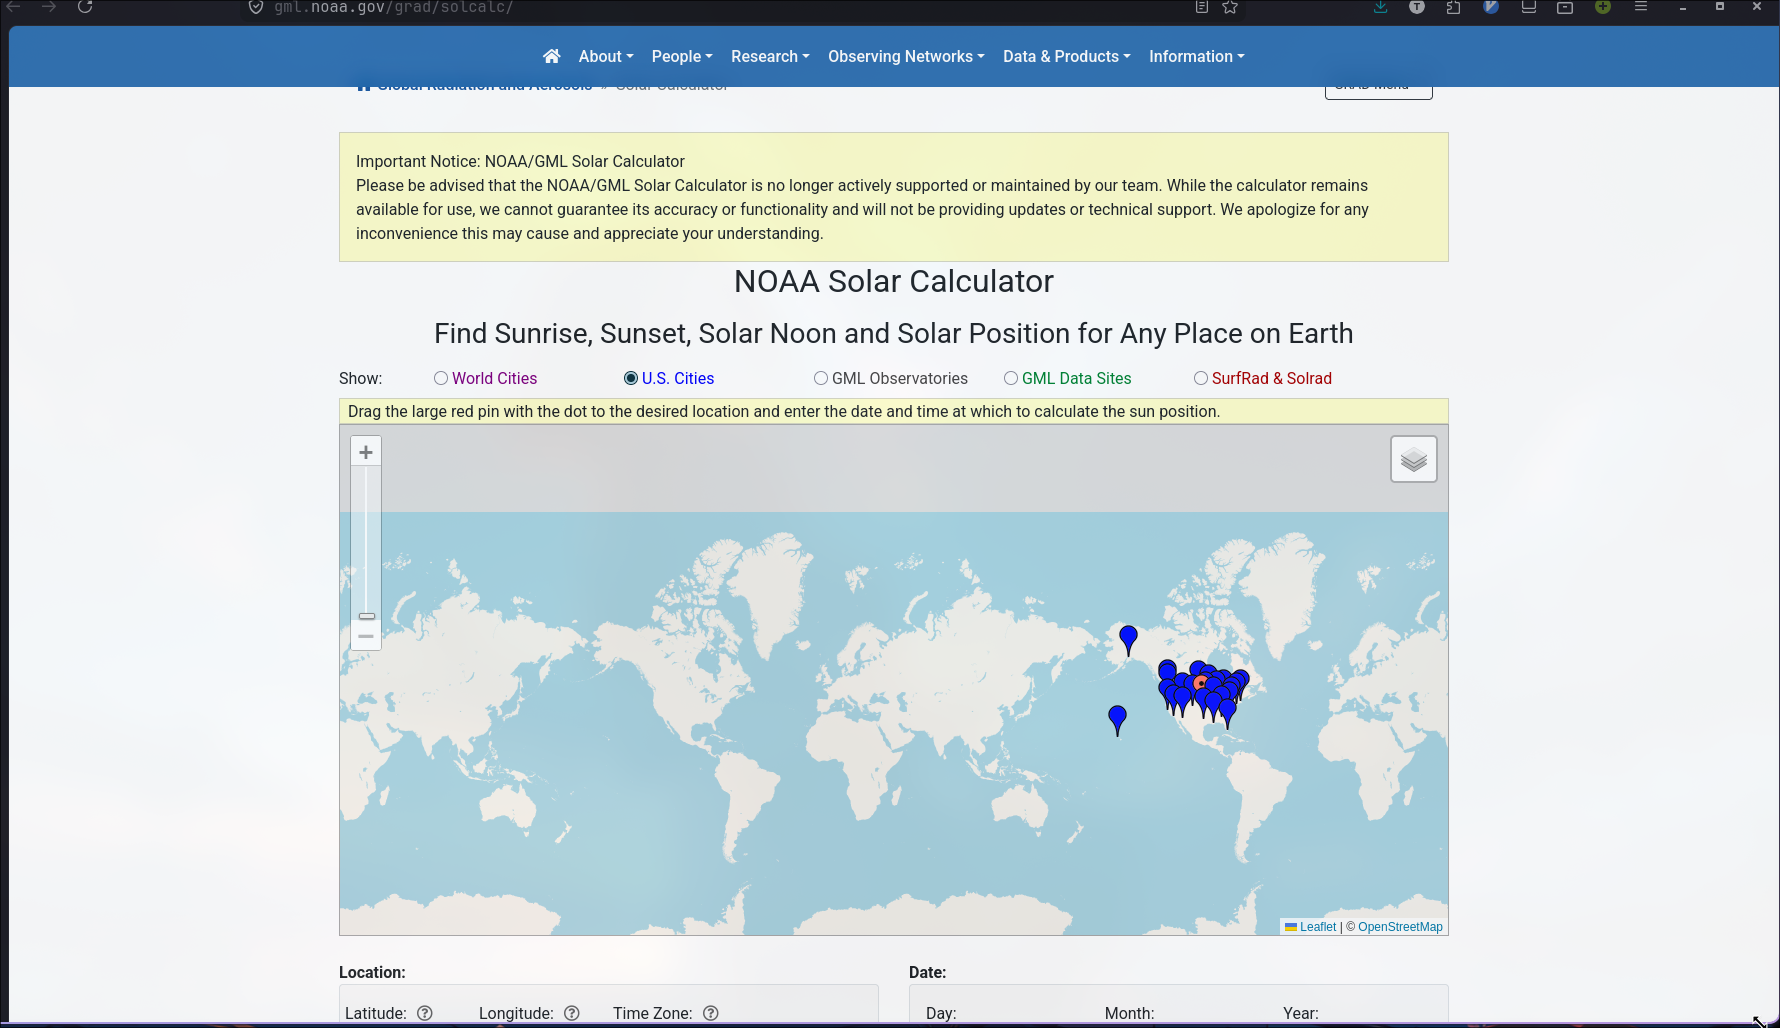
\includegraphics[width=0.85\textwidth]{images/noaa_solar_calculator_real_screenshot.png}
    \caption{Ảnh chụp màn hình thật trang \url{https://gml.noaa.gov/grad/solcalc/} — NOAA Solar Calculator (Global Monitoring Laboratory), công cụ chính thức tính vị trí mặt trời (sunrise/sunset/solar position) mà công thức \texttt{tinh\_goc\_mat\_troi()} trong dự án dựa theo}
    \label{fig:noaa_solar_calc}
\end{figure}

Để chuẩn hóa chu kỳ ngày và triệt tiêu trễ pha theo góc chiếu mặt trời, hệ thống sử dụng mô hình Clear-Sky Haurwitz:
\begin{equation}
    GHI_{\text{haurwitz}} = 1098 \times \sin(h) \times \exp\left(-\frac{0.057}{\sin(h)}\right) \quad (\text{W/m}^2)
\end{equation}
\textit{\textbf{Nguồn bài báo tham khảo:} B. Haurwitz (1945)~\cite{haurwitz1945}, "Insolation in Relation to Cloudiness and Cloud Density", \textit{Journal of Meteorology}, Vol. 2, pp. 154--166; và M. D. Bailey et al. (2024)~\cite{bailey2024downscaling}, "Temporal and Spatial Downscaling for Solar Radiation", ArXiv: \url{https://arxiv.org/abs/2405.11046}}

\begin{figure}[htbp]
    \centering
    \includegraphics[width=0.82\textwidth]{images/paper_lauret_clearsky_index_khung.png}
    \caption{Ảnh chụp trang đầu của bài báo Lauret et al. (2022)~\cite{lauret2022clearsky}, DOI: 10.3390/solar2040026. Ngay trong tiêu đề và nội dung, paper đặt bài toán so sánh dự báo dựa trên \textit{clear-sky index} với \textit{clearness index}; nhóm lấy đúng ngữ cảnh chuẩn hóa biến thiên mặt trời này để xây dựng đặc trưng $K_t$. Paper không mô tả nguyên xi thuật toán downscale của dự án. Việc tái tạo dữ liệu dưới-giờ được nhóm thực nghiệm riêng, đồng thời tham khảo bối cảnh disaggregation từ Grantham et al. (2017)~\cite{grantham2017synthetic}, DOI: 10.1016/j.solener.2017.03.026.}
    \label{fig:paper_lauret}
\end{figure}

\begin{figure}[htbp]
    \centering
    \includegraphics[width=0.9\textwidth]{images/paper_mcdowell2018_subhourly_solar.png}
    \caption{Ảnh chụp trang đầu của bài báo McDowell, Letellier-Duchesne \& Kummert (2018)~\cite{mcdowell2018subhourly}, pp. 518--525.}
    \label{fig:paper_mcdowell2018}
\end{figure}

\begin{figure}[htbp]
    \centering
    \includegraphics[width=0.75\textwidth]{images/paper_mcdowell2018_method_section.png}
    \caption{Trích trang 2 thật (mục "POSSIBLE METHODS" và đoạn văn ngay trước đó) của cùng bài báo — trình bày rõ nội dung ý tưởng: dữ liệu bức xạ chỉ có tổng theo giờ, bằng 0 lúc mặt trời mọc/lặn, cần thuật toán tái tạo hình dạng dưới-giờ hợp lý mà vẫn khớp tổng giờ gốc; đoạn văn trích dẫn trực tiếp \textbf{Grantham et al. (2017)~\cite{grantham2017synthetic}} là công trình tạo dữ liệu độ phân giải cao hơn từ dữ liệu giờ — đây là bằng chứng ý tưởng thật (không chỉ tên bài báo) cho bối cảnh khoa học của bài toán downscale mà dự án giải quyết bằng thuật toán riêng (xem ảnh code thật \texttt{add\_downscaled\_radiation()} bên dưới)}
    \label{fig:paper_mcdowell2018_method}
\end{figure}

\begin{figure}[htbp]
    \centering
    \includegraphics[width=0.95\textwidth]{images/code_notebook_add_downscaled_radiation.png}
    \caption{Ảnh chụp thật (không chạy lại, chỉ đọc source đã lưu sẵn) hàm \texttt{add\_downscaled\_radiation()} trong \texttt{srcs/05\_machine\_learning/pipeline/stages/s04b\_downscale\_radiation.py} — đây là thuật toán downscale THẬT của dự án, cùng nguyên lý chung với Grantham et al. (2017)~\cite{grantham2017synthetic} (nhân tỷ lệ chỉ số trời-quang với GHI clear-sky ở độ phân giải cao hơn), nhưng có 3 điểm khác biệt tự phát triển: (1) ranh giới khối giờ xác định TỰ ĐỘNG từ dữ liệu (không giả định cố định phút :00/:15); (2) chỉ downscale khối nào có tỷ lệ biến thiên $GHI_{cs}$ max/min $\le 1.5$ lần, khối không đạt giữ nguyên bậc thang gốc thay vì ép downscale sai; (3) không dùng ngưỡng tuyệt đối $\sin(elevation)$ mà dùng tỷ lệ đối xứng max/min trong khối — cả 3 điểm này được kiểm chứng bằng tay trên dữ liệu thật (ghi trong docstring), không sao chép nguyên văn công thức từ paper nào}
    \label{fig:code_downscale}
\end{figure}

\begin{figure}[htbp]
    \centering
    \includegraphics[width=0.88\textwidth]{images/paper_haurwitz_1945_khung.png}
    \caption{Ảnh chụp trang đầu của bài báo Haurwitz (1945)~\cite{haurwitz1945}, \textit{Journal of Meteorology} 2(3), 154--166. Abstract nêu các quan hệ thực nghiệm giữa insolation, cloudiness, cloud density và air mass. Đây là nguồn gốc bối cảnh mô hình Haurwitz; ảnh không chứa cặp hằng số $1098/0.057$, nên công thức triển khai của dự án được quy về phiên bản Haurwitz trong pvlib, không gán hai hằng số đó trực tiếp cho đoạn ảnh.}
    \label{fig:paper_haurwitz}
\end{figure}

\begin{itemize}
    \item $GHI_{\text{haurwitz}}$: Bức xạ mặt trời toàn phần lý thuyết chiếu xuống mặt phẳng ngang khi trời hoàn toàn trong ($\text{W/m}^2$).
    \item $1098 \text{ W/m}^2$: Hằng số bức xạ quang phổ mặt trời tại bề mặt Trái Đất sau khi qua bầu khí quyển chuẩn.
    \item $h$: Góc nâng mặt trời so với chân trời (\textit{Solar Elevation Angle}, đơn vị: độ $^\circ$).
    \item $\sin(h)$: Tỷ lệ phần trăm diện tích tia nắng chiếu vuông góc xuống mặt đất ($0 \le \sin(h) \le 1$).
    \item $0.057$: Hệ số suy hao quang học của bầu khí quyển chuẩn (\textit{Atmospheric Extinction Coefficient}).
\end{itemize}

\subsection{Sản lượng điện nén cấp Giờ ($E_{hourly}$)}
\begin{equation}
    E_{hourly} = \sum_{t=1}^{4} E_{15min, t} \quad (\text{kWh})
\end{equation}
\textit{\textbf{Ghi chú:} Đây là phép tổng hợp năng lượng vật lý đơn giản (cộng 4 giá trị 15 phút thành 1 giờ), không cần trích dẫn học thuật riêng.}

\subsection{Tỷ số hiệu suất trạm phát (Performance Ratio - PR)}
\begin{equation}
    \text{PR} = \begin{cases} 
      0 & \text{khi } G_{\text{poa}} \le 0 \quad (\text{ban đêm}) \\
      \frac{E_{\text{actual}}}{P_{\text{stc}} \times (G_{\text{poa}} / 1000) \times \Delta t} & \text{khi } G_{\text{poa}} > 0
    \end{cases}
\end{equation}
\textit{\textbf{Nguồn tiêu chuẩn tham khảo:} Tiêu chuẩn Quốc tế IEC 61724-1~\cite{iec61724}, "Photovoltaic System Performance Monitoring — Guidelines for Measurement, Data Exchange and Analysis".}

\begin{itemize}
    \item $E_{\text{actual}}$: Sản lượng điện thực tế trạm quang điện phát được trong khoảng thời gian $\Delta t$ ($\text{kWh}$).
    \item $P_{\text{stc}}$: Công suất lắp đặt định mức của trang trại ở điều kiện tiêu chuẩn ST ($1000 \text{ W/m}^2, 25^\circ\text{}$) ($\text{kWp}$).
    \item $G_{\text{poa}}$: Bức xạ mặt trời đo trên mặt phẳng nghiêng tấm pin (\textit{Plane of Array Irradiance}, $\text{W/m}^2$).
    \item $1000 \text{ W/m}^2$: Bức xạ chuẩn ST dùng làm mốc so sánh hiệu suất tấm pin.
    \item $\Delta t$: Khoảng thời gian đo tích phân ($0.25\text{h} = 15\text{m}$).
    \item \textbf{Ý nghĩa nghiệp vụ PR:} Đo lường tỷ lệ tổn thất kỹ thuật (bụi bẩn, suy giảm Inverter, quá nhiệt tấm pin). Chuẩn trạm vận hành tốt phải đạt $\text{PR} \ge 80\%$.
\end{itemize}

\subsection{Hệ số công suất khai thác (Capacity Factor - F)}
\begin{equation}
    F = \frac{E_{daily}}{P_{stc} \times 24} \times 100\%
\end{equation}
\textit{\textbf{Nguồn tham khảo 1:} NREL, \textit{Annual Technology Baseline (ATB) 2021 — Utility-Scale PV}~\cite{nrelatb2021pv}, \url{https://atb.nrel.gov/electricity/2021/utility-scale_pv}. NREL định nghĩa Capacity Factor là tỷ lệ giữa sản lượng năng lượng trung bình thực tế và sản lượng có thể tạo ra nếu nhà máy vận hành ở công suất định mức trong mọi giờ của cùng khoảng thời gian; công thức trên áp dụng định nghĩa tổng quát này cho một ngày.}

\textit{\textbf{Nguồn tham khảo 2:} P. Denholm (2013)~\cite{denholm2013capacity}, ``Solar Energy and Capacity Value,'' NREL/FS-6A20-57582, DOI: \url{https://doi.org/10.2172/1094876}. Tài liệu giải thích thêm rằng công suất hệ PV có thể được biểu diễn theo A hoặc D; vì vậy tử số và mẫu số phải dùng nhất quán cùng cơ sở công suất. Ảnh chụp nguyên bản trang 2, mục ``Defining Capacity-Related Terms'' được đối chiếu từ hồ sơ lưu trữ chính thức của UNT: \url{https://digital.library.unt.edu/ark:/67531/metadc844164/}.}


\section[KHÁM PHÁ DỮ LIỆU EDA \& OUTLIER GMM-IF]{PHÂN TÍCH KHÁM PHÁ DỮ LIỆU (EDA) VÀ\\THUẬT TOÁN PHÁT HIỆN OUTLIER (GMM-IF)}

Trước khi tiến hành trích xuất đặc trưng (Feature Engineering) và huấn luyện mô hình dự báo, toàn bộ quy trình xử lý dữ liệu trong thư mục \texttt{notebooks/EDA/} và \texttt{srcs/02\_transform/} được thực hiện với 6 notebook EDA chuyên sâu độc lập nhằm khai phá mọi khía cạnh cấu trúc dữ liệu của 42 trạm quang điện.



\subsection{Tổng Quan Toàn Bộ 6 Notebook Phân Tích EDA trong Dự Án}
Nhóm nghiên cứu đã xây dựng một bộ công cụ EDA toàn diện bao phủ từ thống kê mô tả, phân bố đơn biến, chuỗi thời gian tự tương quan cho đến thuật toán phát hiện bất thường nâng cao:

\begin{enumerate}
    \item \textbf{\texttt{thong\_ke\_mo\_ta.ipynb} \& \texttt{05\_univariate\_plots.py}:} Thống kê mô tả toàn bộ 42 trạm (Trung bình, Trung vị, Độ lệch chuẩn, Độ lệch Skewness, Độ nhọn Kurtosis, các mức Phân vị) và Đồ thị Phân bố Đơn biến (KDE, Histogram, Boxplot).
    \item \textbf{\texttt{pattern\_discovery.ipynb}:} Phân tích mẫu hình phát điện ngày đêm, nhịp sinh học mặt trời, tác động của chỉ số mây che (\textit{Cloud Cover Attenuation}) và bức xạ Clear-Sky.
    \item \textbf{\texttt{v1\_AF\_PAF.ipynb}:} Phân tích Tự tương quan (AF) và Tự tương quan Riêng phần (PAF) đa độ trễ ($k=1$ đến $k=288$) để phát hiện hiện tượng sao chép quá khứ.
    \item \textbf{\texttt{v2\_\_correlation\_heatmap.ipynb}:} Phân tích ma trận tương quan Spearman \& Pearson giữa các biến khí tượng, góc nâng mặt trời và sản lượng điện.
    \item \textbf{\texttt{srcs/02\_transform/02\_generate\_outliers/02\_gmm\_if.py}:}\\Thực thi pipeline phát hiện bất thường hiện tại gồm Decision Tree segmentation, GMM theo segment, Isolation Forest và Physical Guardrail. Hàm \texttt{explain\_outlier\_row()} sinh trực tiếp trường \texttt{outlier\_reason}.
    \item \textbf{\texttt{05\_validate\_gmm\_if\_metrics.py} \& \texttt{06\_regenerate\_report\_figures.py}:}\\Đọc audit hiện tại, ghi metrics và sinh lại bộ hình report từ các file số trong \texttt{reports/final\_rolling\_compare/}; không đọc các PNG lịch sử. Các reason code không phải là ba nhãn loại trừ nhau; một dòng có thể mang nhiều mã nối bằng dấu \texttt{+}.
\end{enumerate}

\subsection{Phân Tích Thống Kê Mô Tả \& Phân Bố Đơn Biến}
Phân tích thống kê trên 42 trạm quang điện cho thấy dữ liệu sản lượng điện $y$ và bức xạ $GHI$ có đặc tính phi chuẩn rất mạnh:

\begin{figure}[htbp]
    \centering
    \includegraphics[width=0.82\textwidth]{images/eda_univariate_distributions.png}
    \caption{Hình 2.1 (Kết quả Thực nghiệm từ Notebook \texttt{thong\_ke\_mo\_ta.ipynb}): Đồ thị Phân bố Đơn biến Sản lượng thô $y$ và Bộ lọc Ban ngày}
    \label{fig:eda_univariate}
\end{figure}
\textbf{Ý nghĩa \& Insight Đồ thị Phân bố Đơn biến (Hình \ref{fig:eda_univariate}):}
\begin{itemize}
    \item \textbf{Hiện tượng Lệch Phải Cực Độ (Heavy Right-Skewness, $\text{Skewness} > 1.8$):} Do thời gian ban đêm và các khung giờ sáng sớm/chiều tà chiếm hơn 50\% số lượng quan sát với giá trị $y = 0.0 \text{ kWh}$.
    \item \textbf{Độ nhọn Kurtosis cao ($\text{Kurtosis} > 3.5$):} Sản lượng phát tập trung nổ bùng vào dải hẹp quanh giữa trưa (11:30 -- 12:30).
    \item \textbf{ Kỹ thuật FE:} Kết quả này đặt ra yêu cầu bắt buộc phải lọc bỏ các số 0 ban đêm (\texttt{is\_daylight = True}) và áp dụng cơ chế chuẩn hóa mục tiêu \textbf{Target Physical Normalization} $k_{\text{target}} = \frac{y}{P_{\text{capacity}} \times \max(\sin(h), 0.02)}$ để biến đổi phân bố về dạng đều $[0, 1.5]$.
\end{itemize}

\subsection{Phân Tích Mẫu Hình Phát Điện \& Tác Động Mây Che}
Khám phá quy luật phát điện giữa ngày Bầu trời trong (Clear-sky) và ngày Mây mù biến động (Overcast):

\begin{figure}[htbp]
    \centering
    \includegraphics[width=0.82\textwidth]{images/eda_pattern_clear_vs_cloudy.png}
    \caption{Hình 2.2 (Kết quả Thực nghiệm từ Notebook \texttt{pattern\_discovery.ipynb}): Phân tích So sánh Quy luật Phát điện Ngày Bầu trời Trong vs Mây Che}
    \label{fig:eda_pattern_clear_cloudy}
\end{figure}
\textbf{Ý nghĩa \& Insight Đồ thị Mẫu hình Bức xạ (Hình \ref{fig:eda_pattern_clear_cloudy}):}
\begin{itemize}
    \item \textbf{Ngày Bầu trời trong:} Chuỗi sản lượng tạo thành đường cong Parabol hoàn hảo, đỉnh đạt tối đa tại mốc $12:00$.
    \item \textbf{Ngày Mây mù biến động:} Bức xạ $GHI$ suy giảm đột ngột từ $800 \text{ W/m}^2$ xuống $< 150 \text{ W/m}^2$ trong vòng 15 phút, kéo theo sản lượng $y$ tụt dốc tương ứng.
    \item \textbf{ Kỹ thuật FE:} Đây là luận cứ để tính toán chỉ số \textbf{Clear-Sky Index} $K_t = \frac{GHI_{\text{raw}}}{GHI_{\text{clearsky}}}$ và biến tương tác tích \texttt{rad\_x\_sinelev}, giúp mô hình phản ứng tức thì với các biến động mây ngắn hạn mà không bị trễ pha.
\end{itemize}


Khám phá quy luật phát điện giữa ngày Bầu trời trong (Clear-sky) và ngày Mây mù biến động (Overcast):
\begin{itemize}
    \item \textbf{Ngày Bầu trời trong:} Chuỗi sản lượng tạo thành đường cong Parabol hoàn hảo, đỉnh đạt tối đa tại mốc $12:00$.
    \item \textbf{Ngày Mây mù biến động:} Bức xạ $GHI$ suy giảm đột ngột từ $800 \text{ W/m}^2$ xuống $< 150 \text{ W/m}^2$ trong vòng 15 phút, kéo theo sản lượng $y$ tụt dốc tương ứng.
    \item \textbf{ Kỹ thuật FE:} Đây là luận cứ để tính toán chỉ số **Clear-Sky Index** $K_t = \frac{GHI_{\text{raw}}}{GHI_{\text{clearsky}}}$ và biến tương tác tích \texttt{rad\_x\_sinelev}, giúp mô hình phản ứng tức thì với các biến động mây ngắn hạn mà không bị trễ pha.
\end{itemize}


\subsubsection[Kết Quả GMM-IF trên Pipeline]{Kết Quả Chạy Thực Tế Thuật Toán GMM-IF\\trên audit GMM-IF hiện tại}
Các metrics được tái sinh bằng \texttt{05\_validate\_gmm\_if\_metrics.py} từ \texttt{reports/final\_rolling\_compare/03\_gmm\_if\_full\_audit.csv}; file \texttt{11\_gmm\_if\_model\_metrics.log} ghi nhận kết quả lọc bất thường trên toàn bộ ma trận dữ liệu của 42 trạm:

\begin{itemize}
    \item \textbf{Quy mô dữ liệu:} Nhật ký ghi nhận $2{,}731{,}946$ dòng quan sát 15 phút của 42 trạm, từ \texttt{2020-01-01 00:15:00} đến \texttt{2022-04-23 23:45:00}.
    \item \textbf{Ứng viên GMM:} GMM theo các segment do Decision Tree sinh ra đánh dấu $26{,}496$ dòng có mật độ tương đối cục bộ dưới ngưỡng $P_{\text{GMM}} < 0.02$.
    \item \textbf{Ứng viên Isolation Forest:} Isolation Forest đánh dấu $37{,}518$ dòng theo cơ chế contamination cấu hình ở mức $0.03$; log không dùng một ngưỡng điểm $S_{\text{IF}} > 0.65$ làm nhãn cuối.
    \item \textbf{Đồng thuận GMM--IF:} Có $6{,}178$ dòng đồng thời có cờ GMM và IF, tương đương $0.226139\%$ tổng dữ liệu.
    \item \textbf{Physical Guardrail:} Có $27{,}822$ dòng thỏa ít nhất một điều kiện vật lý ($1.018395\%$ tổng dữ liệu). Đây là một nhánh bổ sung được hợp nhất bằng phép OR, không phải một loại outlier thứ ba; các cờ vật lý có thể chồng lấn.
    \item \textbf{Nhãn cuối:} \texttt{final\_outlier = GMM\_IF\_CONSENSUS OR physical\_guardrail}, gồm $33{,}280$ dòng ($1.218179\%$). Phần còn lại là $2{,}698{,}666$ dòng \texttt{keep\_raw} ($98.781821\%$).
\end{itemize}

\begin{table}[htbp]
\centering
\caption{Các tầng phát hiện và hai trạng thái cuối của audit GMM--IF hiện tại (metrics tái sinh từ audit local)}
\label{tab:gmm_if_log_results}
\small
\begin{tabularx}{\linewidth}{l r r X}
\toprule
\textbf{Tầng/trạng thái} & \textbf{Số dòng} & \textbf{Tỷ lệ} & \textbf{Vai trò} \\
\midrule
Decision Tree segmentation & 2,731,946 & 100.000\% & Phân vùng profile; không phải nhãn outlier. \\
GMM low probability & 26,496 & 0.969858\% & Tập ứng viên cục bộ. \\
Isolation Forest & 37,518 & 1.373307\% & Tập ứng viên độc lập toàn cục. \\
GMM $\cap$ IF & 6,178 & 0.226139\% & Nhánh đồng thuận của hai bộ phát hiện. \\
Physical Guardrail & 27,822 & 1.018395\% & Nhánh kiểm tra vật lý bổ sung; các reason có thể chồng lấn. \\
\textbf{Final outlier} & \textbf{33,280} & \textbf{1.218179\%} & Hợp của đồng thuận GMM--IF và Physical Guardrail. \\
\textbf{Keep raw} & \textbf{2,698,666} & \textbf{98.781821\%} & \texttt{gmm\_if\_outlier\_flag = 0}; không bị pipeline gắn cờ. \\
\midrule
\multicolumn{4}{l}{\textit{Suy ra từ hai tổng nhánh: 720 dòng đồng thời thuộc consensus và physical guardrail.}} \\
\bottomrule
\end{tabularx}
\end{table}

\textbf{Ý nghĩa Data Science:} Audit hiện tại gắn cờ **1.218179\%** quan sát (33,280/2,731,946 dòng) và giữ lại **98.781821\%** quan sát không bị gắn cờ để huấn luyện mô hình LightGBM. Con số này phản ánh mức độ lọc (tỷ lệ dữ liệu bị đánh dấu), \textbf{không tự chứng minh độ chính xác (precision)} của nhãn outlier — muốn khẳng định các điểm bị loại thực sự là nhiễu cần đối chiếu nhãn thật hoặc kiểm tra thủ công, việc này chưa được thực hiện. Snapshot cũ có $6{,}962$ dòng final là kết quả trước khi bổ sung/chạy nhánh \texttt{PHYSICAL\_OVER\_CAPACITY}; không trộn snapshot đó vào bảng hiện tại.

\subsection{Làm sạch Lưới Thời Gian 15 Phút Causal (Reindex Continuous Grid)}
\begin{figure}[H]
    \centering
    \includegraphics[width=0.95\textwidth]{images/code_pipeline_build_grid.png}
    \caption{Mã nguồn dựng lưới thời gian liên tục 15 phút trong \texttt{srcs/05\_machine\_learning/pipeline/stages/s01a\_build\_grid.py}: hàm \texttt{reindex\_luoi()} sinh trục thời gian đầy đủ cho từng trạm bằng \texttt{pd.date\_range}, đánh dấu dòng được chèn thêm qua cột \texttt{timestamp\_was\_inserted}; hàm \texttt{ffill\_thoi\_tiet()} lan truyền giá trị khí tượng theo chiều tiến (\texttt{ffill}) trong phạm vi từng trạm, giữ nguyên tắc nhân quả}
    \label{fig:code_build_grid}
\end{figure}

\begin{figure}[H]
    \centering
    \includegraphics[width=0.95\textwidth]{images/code_pipeline_fill_energy.png}
    \caption{Mã nguồn thang điền khuyết sản lượng trong \texttt{srcs/05\_machine\_learning/pipeline/stages/s01b\_fill\_energy.py}. Thứ tự ưu tiên: \texttt{night\_zero} (ban đêm gán 0) $\rightarrow$ \texttt{causal\_day\_persistence} (lấy cùng khung giờ ngày trước) $\rightarrow$ \texttt{causal\_week\_persistence} $\rightarrow$ \texttt{causal\_profile\_median}. Mọi nguồn đều nhìn về quá khứ và được ghi lại trong cột \texttt{energy\_source}, nhờ đó mọi chỉ số công bố đều lọc được về đúng phần dữ liệu đo thật}
    \label{fig:code_fill_energy}
\end{figure}

Dữ liệu thô từ 42 trạm quang điện tồn tại các khoảng trống thời gian (\textit{missing timestamp gaps}). Để đảm bảo tính liên tục của chuỗi thời gian:
\begin{enumerate}
    \item \textbf{Reindex Lưới 15 phút:} Tạo lại trục thời gian hoàn chỉnh $15 \text{m}$ cho từng trạm từ mốc bắt đầu đến kết thúc.
    \item \textbf{Gán cờ Provenance (\texttt{energy\_source}):} Đánh dấu rõ các dòng thực đo (\texttt{measured}) và các dòng nội suy/chèn thêm (\texttt{etl\_imputed}) để ngăn hiện tượng rò rỉ dữ liệu tương lai (\textit{Causal Leakage}).
    \item \textbf{Forward Fill Causal thời tiết:} Chỉ sử dụng các giá trị thời tiết đã quan sát trước đó (\texttt{ffill}) kéo sang các slot mới chèn.
\end{enumerate}


\subsection{Thuật toán Phát hiện Outlier GMM-IF Fusion (Thích nghi từ Ngữ cảnh IEEE Access 2025)}
\begin{figure}[H]
    \centering
    \includegraphics[width=0.95\textwidth]{images/code_pipeline_weather_causal.png}
    \caption{Mã nguồn ghép lại dữ liệu khí tượng theo quy tắc nhân quả trong \texttt{srcs/05\_machine\_learning/pipeline/stages/s01d\_weather\_causal.py} — mỗi dòng tại thời điểm $T$ chỉ nhận khối khí tượng của giờ đã kết thúc, xác định bằng \texttt{floor(\"h\")}. Phép kiểm ở cuối hàm dừng chương trình nếu còn bất kỳ dòng nào tham chiếu khí tượng của tương lai, và nhãn \texttt{hour\_causal\_floor} chỉ được đặt sau khi phép kiểm này đạt}
    \label{fig:code_weather_causal}
\end{figure}

Không sử dụng hình IQR/Rolling-IQR trong kết quả hiện tại vì đó là artefact của pipeline cũ, không phải output của audit GMM--IF hiện tại. Kết quả hiện tại được đọc từ các cờ của file \texttt{02\_gmm\_if.py}: đồng thuận GMM--IF dùng phép AND, sau đó hợp với Physical Guardrail bằng phép OR để tạo nhãn cuối.

Li et al. (2025)~\cite{li2025gmmif} cung cấp ngữ cảnh kết hợp phân đoạn, GMM và Isolation Forest cho dữ liệu phát điện PV; từ đó dự án thiết kế lại luật đồng thuận phù hợp dữ liệu 42 trạm:
\begin{equation}
    \text{Consensus}(x_i) = \mathbb{I}\left(p_{\text{GMM}}(x_i | \text{Segment}_k) < \theta_{\text{gmm}}\right) \land \mathbb{I}\left(\text{IF\_flag}(x_i) = 1\right)
\end{equation}
\textit{\textbf{Ngữ cảnh lấy từ paper:} Abstract của Xin Li et al. (2025)~\cite{li2025gmmif}, "Outlier Detection of Photovoltaic Power Generation System Data Based on GMM-IF Algorithm", nêu rõ chiến lược dùng cây quyết định để phân đoạn dữ liệu thành các vùng gần Gaussian và tích hợp Isolation Forest làm cơ chế quyết định chi tiết. Công thức đồng thuận, các ngưỡng và kết quả bên dưới là phần nhóm thực nghiệm lại, không phải chép nguyên thông số của paper.}\\
\url{https://doi.org/10.1109/ACCESS.2025.3581641}

\begin{itemize}
    \item $x_i$: Vector điểm dữ liệu quan sát tại mốc thời gian $i$ (bao gồm sản lượng $y_i$ và bức xạ $GHI_i$).
    \item $\text{Segment}_k$: Phân đoạn profile ngày thứ $k$ do Cây quyết định tạo ra, nhằm làm phân bố cục bộ gần Gaussian hơn.
    \item $p_{\text{GMM}}(x_i | \text{Segment}_k)$: Mật độ hỗn hợp GMM tại quan sát $x_i$, dùng phát hiện điểm có mật độ cục bộ thấp.
    \item $\theta_{\text{gmm}} = 0.02$: Ngưỡng mật độ do nhóm hiệu chỉnh trên dữ liệu dự án.
    \item $S_{\text{IF}}(x_i)$: Điểm/nhãn bất thường của Isolation Forest $\Rightarrow$ Dùng đánh giá độ cô lập không gian toàn cục.
    \item \texttt{gmm\_if\_if\_contamination} $= 0.03$: Tỷ lệ contamination cấu hình cho Isolation Forest trong file YAML hiện tại; không diễn giải thành một ngưỡng điểm $0.65$.
    \item $\mathbb{I}(\cdot)$: Hàm chỉ thị (Indicator Function) $\Rightarrow$ Trả về $1$ nếu điều kiện đúng, $0$ nếu sai.
    \item $\land$: Phép toán logic AND $\Rightarrow$ Bắt buộc CẢ GMM VÀ IF đồng thời đồng thuận mới kích hoạt cờ trung gian \texttt{gmm\_if\_consensus\_flag = 1}. Nhãn cuối dùng \texttt{gmm\_if\_consensus\_flag OR physical\_rule\_flag}.
\end{itemize}

\begin{figure}[htbp]
    \centering
    \includegraphics[width=0.92\textwidth]{images/gmm_if_combined_theory_diagram.png}
    \caption{(Sơ đồ Lý thuyết Hợp nhất) Cơ sở Khoa học Thuật toán Outlier GMM--IF Fusion: (Trên) Mô hình Hỗn hợp Gauss GMM xấp xỉ phân bố và ngưỡng mật độ $p(x)<\theta$; (Dưới) Mô hình Isolation Forest đánh giá độ dài đường đi cô lập $h(x)$}
    \label{fig:gmm_if_combined_theory}
\end{figure}
\textbf{Ý nghĩa \& Insight Đồ thị Hợp nhất GMM--IF (Hình \ref{fig:gmm_if_combined_theory}):} Biểu đồ phía trên thể hiện cách mô hình GMM xấp xỉ phân bố sản lượng điện bằng hỗn hợp 2 phân bố chuẩn Gaussian với ngưỡng mật độ $\theta = 0.02$. Biểu đồ phía dưới mô tả cơ chế Isolation Forest: (A) Phân chia không gian ngẫu nhiên; (B) Đồ thị độ dài đường đi $h(x)$ — \textit{trong ví dụ minh họa của sơ đồ}: điểm bình thường có đường đi sâu hơn ($h \approx 12$), điểm Outlier có đường đi nông hơn ($h \approx 2$), cho Anomaly Score $\approx 1.0$. Phép kết hợp giao (GMM $\cap$ IF) giúp loại triệt để báo động giả trên 42 trạm quang điện.

\begin{figure}[htbp]
    \centering
    \includegraphics[width=0.82\textwidth]{images/gmm_if_outlier_diagram.png}
    \caption{(Sơ đồ Lý thuyết của dự án) Quy trình 4 bước GMM--IF Fusion được thích nghi từ ngữ cảnh phân đoạn GMM--IF của Li et al. (2025)~\cite{li2025gmmif}}
    \label{fig:gmm_if_diagram}
\end{figure}
\textbf{Ý nghĩa \& Insight Kiến trúc GMM-IF (Hình \ref{fig:gmm_if_diagram}):} Paper Li et al. (2025)~\cite{li2025gmmif} là nguồn của ngữ cảnh phân đoạn GMM--IF; sơ đồ này mô tả phiên bản nhóm đã triển khai lại cho dự án. GMM kiểm tra mật độ cục bộ, Isolation Forest kiểm tra độ cô lập toàn cục, còn phép giao hai cờ là lựa chọn thực nghiệm nhằm hạn chế báo động giả trong thời gian bức xạ biến động cao.

\begin{enumerate}
    \item \textbf{Bước 1 --- Cây Quyết Định Phân Đoạn Profile Ngày (Decision Tree Segmentation):} Dùng Cây quyết định hồi quy chia profile ngày phát điện thành các phân đoạn (\textit{Segments}). Kết quả thực nghiệm trên toàn bộ 42 trạm: $R^2$ trung bình $= 0.758$ (min $0.606$, max $0.826$).
    \item \textbf{Bước 2 --- GMM trên từng Segment:} Khởi tạo mô hình GMM riêng cho từng Segment. Các điểm có mật độ tương đối $P_{\text{GMM}}$ cực thấp được coi là ứng viên bất thường; trong code, mật độ được chuẩn hóa theo mật độ lớn nhất trong segment, không phải posterior probability tuyệt đối.
    \item \textbf{Bước 3 --- Isolation Forest Kiểm định Toàn cục:} Huấn luyện mô hình Isolation Forest trên toàn bộ chuỗi thời gian của trạm để đánh giá độ cô lập không gian.
    \item \textbf{Bước 4 --- Gắn cờ cuối:} Cờ trung gian \texttt{gmm\_if\_consensus\_flag} là giao GMM $\cap$ IF; cờ cuối \texttt{is\_outlier} là hợp của cờ trung gian này với \texttt{physical\_rule\_flag}.
\end{enumerate}

\begin{figure}[htbp]
    \centering
    \includegraphics[width=0.82\textwidth]{images/decision_tree_r2_by_site.png}
    \caption{Kết quả thực nghiệm thật (42 trạm): $R^2$ phân đoạn Decision Tree theo từng site — trích từ \texttt{pictures/final\_rolling\_compare/09\_step1\_decision\_tree\_energy\_r2\_by\_site.png}}
    \label{fig:dt_r2_by_site}
\end{figure}

\subsubsection{Lý do chấp nhận mức $R^2$ và vai trò của GMM--IF}
Chỉ số $R^2$ ở Bước 1 không phải độ chính xác dự báo và cũng không phải precision/recall của bộ phát hiện outlier. Trong file \texttt{04\_validate\_decision\_tree\_r2.py}, mỗi dòng ban ngày được so sánh với trung bình sản lượng của chính \texttt{segment\_id}; do đó chỉ số này đo mức độ các segment do Decision Tree tạo ra giữ được cấu trúc profile phát điện của từng site.

Với cách diễn giải đó, $R^2_{\text{energy}}$ trung bình $=0.758$ nghĩa là các segment giải thích được khoảng $75.8\%$ biến thiên sản lượng ban ngày trong phép kiểm tra nội bộ; site thấp nhất vẫn đạt $0.606$ và site cao nhất đạt $0.826$. Các giá trị đều dương và nằm ở mức trung bình--cao, cho thấy phân đoạn tốt hơn một mô hình chỉ dùng trung bình chung của site, nhưng chưa hoàn hảo vì sản lượng còn chịu ảnh hưởng của mây, bức xạ, thời tiết và nhiễu đo. Vì mục tiêu của Bước 1 là tạo các vùng cục bộ gần đồng nhất để chạy GMM, mức này đủ để dùng làm bước phân đoạn ứng viên; báo cáo không gọi đây là độ chính xác dự báo và không áp đặt một ngưỡng pass/fail chưa được kiểm nghiệm.

Chỉ số $R^2$ của residual thấp hơn ($0.118$--$0.346$, trung bình $0.187$) cũng phù hợp với vai trò của nó: residual là phần biến động còn lại sau khi điều kiện bức xạ được đưa vào, nên chứa nhiều nhiễu thời tiết và sai số cảm biến hơn. Vì vậy, residual $R^2$ thấp không phủ định segmentation; nó nhắc rằng GMM--IF phải được dùng như một cơ chế sàng lọc nhiều lớp chứ không phải một mô hình hồi quy thay thế.

Đối với GMM, tiêu chí chấp nhận không phải $R^2$ mà là mật độ tương đối cục bộ trong từng segment. GMM dùng $P_{\text{GMM}}<0.02$ để tạo $26{,}496$ ứng viên; sau khi yêu cầu Isolation Forest đồng thuận, còn $6{,}178$ dòng, tức $23.316727\%$ số ứng viên GMM sống sót qua phép AND. Điều này cho thấy lớp đồng thuận làm giảm cảnh báo đơn lẻ, nhưng không được diễn giải thành precision vì dự án chưa có nhãn outlier do con người xác nhận.

Đối với Isolation Forest, file YAML đặt \texttt{gmm\_if\_if\_contamination}=0.03, tức ngân sách vận hành để đánh dấu các điểm có độ cô lập cao, không phải một ngưỡng score chuẩn hóa. IF tạo $37{,}518$ ứng viên và $6{,}178$ dòng cùng được GMM xác nhận, tương đương $16.466763\%$ ứng viên IF. Metrics còn cho thấy score IF trung bình của các dòng final là $0.511737$, so với $0.407825$ ở dòng bình thường, chênh lệch $0.103912$; đây là bằng chứng giám sát khả năng tách hạng của score, không phải chứng nhận độ chính xác.

Do đó, quyết định giữ GMM--IF trong pipeline dựa trên tính bổ trợ: Decision Tree tạo ngữ cảnh cục bộ, GMM kiểm tra độ lệch trong ngữ cảnh đó, IF kiểm tra độ cô lập toàn cục, còn Physical Guardrail kiểm tra mâu thuẫn vật lý. Khi chưa có ground truth, mức chấp nhận là mức độ nhất quán và khả năng giảm cảnh báo qua các tầng; mọi kết luận về precision/recall vẫn được ghi là chưa xác minh.

\begin{figure}[htbp]
    \centering
    \includegraphics[width=0.82\textwidth]{images/gmm_if_final_outliers_by_site.png}
    \caption{Kết quả thực nghiệm theo site của nhãn cuối GMM--IF: cột tím là số outlier cuối, đường cam là số dòng bị Physical Guardrail gắn cờ. Hình đại diện lấy từ \texttt{Figure\_13\_Step3\_Final\_Outliers\_By\_Site.png}; tổng audit hiện tại là $33{,}280$ final outliers và $27{,}822$ physical guardrail flags.}
    \label{fig:gmm_if_final_outliers}
\end{figure}

\begin{figure}[htbp]
    \centering
    \includegraphics[width=0.85\textwidth]{images/paper_gmmif_2025_titlepage.png}
    \caption{Ảnh chụp trang đầu của bài báo Li et al. (2025)~\cite{li2025gmmif}, \textit{IEEE Access}, DOI: 10.1109/ACCESS.2025.3581641. Abstract của paper nêu rõ một thuật toán GMM--IF phân đoạn: dùng cây quyết định để cấu trúc dữ liệu thành các vùng gần Gaussian, sau đó tích hợp Isolation Forest làm cơ chế ra quyết định chi tiết. Dự án lấy đúng kiến trúc khái niệm này làm ngữ cảnh; các ngưỡng GMM/IF và luật đồng thuận GMM $\cap$ IF được nhóm thiết kế, hiệu chỉnh và kiểm nghiệm lại trên 42 trạm, không trình bày như thông số sao chép nguyên văn từ paper.}
    \label{fig:paper_gmmif}
\end{figure}

\subsection[Phân loại theo outlier\_reason]{Phân loại theo trường \texttt{outlier\_reason} của pipeline hiện tại}
Dựa trên hàm \texttt{explain\_outlier\_row()} trong \texttt{srcs/02\_transform/02\_generate\_outliers/02\_gmm\_if.py}, pipeline không ép mỗi điểm vào một trong ba nhóm loại trừ nhau. Một dòng có thể đồng thời thỏa nhiều điều kiện; khi đó các mã được nối bằng dấu \texttt{+} trong \texttt{outlier\_reason}:
\begin{itemize}
    \item \textbf{\texttt{GMM\_IF\_CONSENSUS}:} GMM đánh dấu xác suất cục bộ thấp và Isolation Forest đồng thời đánh dấu cùng dòng; đây là nhánh đồng thuận thống kê.
    \item \textbf{\texttt{PHYSICAL\_OVER\_CAPACITY}:} Sản lượng 15 phút vượt \texttt{capacity\_kw} $\times 0.25$ giờ; cấu hình hiện tại đặt \texttt{gmm\_if\_over\_capacity\_tolerance = 1.0}. Audit có $26{,}501$ cờ của điều kiện này.
    \item \textbf{\texttt{PHYSICAL\_HIGH\_ENERGY\_NO\_SUN}:} Sản lượng $\geq \max(1.0, 0.20\times\texttt{capacity\_reference\_kw})$ khi \texttt{shortwave\_radiation} $\leq 25$ và \texttt{sunshine\_duration} $\leq 60$. Audit có $36$ cờ.
    \item \textbf{\texttt{PHYSICAL\_HIGH\_ENERGY\_LOW\_RADIATION}:} Sản lượng cao khi \texttt{shortwave\_radiation} $\leq 50$, đồng thời vượt $Q_3 + 4\times\texttt{safe\_IQR}$ và ngưỡng $0.20\times\texttt{capacity\_reference\_kw}$. Audit có $140$ cờ.
    \item \textbf{\texttt{PHYSICAL\_LOW\_ENERGY\_STRONG\_SUN}:} Sản lượng $\leq 5\%$ $p95$ của site khi bức xạ $\geq 700$, thời lượng nắng $\geq 3000$, mức kỳ vọng cao và thấp hơn $Q_1 - 2\times\texttt{safe\_IQR}$. Audit có $57$ cờ.
    \item \textbf{\texttt{PHYSICAL\_DISTRIBUTION\_JUMP}:} Ngoài giờ loại trừ 05, 06, 18; sai lệch vượt $Q_3 + 4\times\texttt{safe\_IQR}$ hoặc thấp hơn $Q_1 - 4\times\texttt{safe\_IQR}$, đồng thời $|\texttt{neighbor\_delta}| \geq \max(0.15\times p95, 1.0)$. Audit có $1{,}202$ cờ.
\end{itemize}
Các tên \texttt{zero\_generation\_daylight} và \texttt{stuck\_sensor} không được hàm \texttt{explain\_outlier\_row()} của file 02 sinh ra trong pipeline mới, nên không dùng làm loại outlier cho kết quả này. Tương tự, \texttt{FINAL\_FLAG} chỉ xuất hiện ở các dòng bối cảnh được in kèm log, không phải một reason code của các dòng outlier cuối.

\subsection[Ý nghĩa nghiệp vụ của Physical Guardrail]{Ý nghĩa nghiệp vụ của các điều kiện Physical Guardrail}
Physical Guardrail là lớp kiểm tra tính hợp lý vật lý bổ sung cho hai bộ phát hiện thống kê. Nó không chứng minh nguyên nhân gốc của lỗi đo; nó chỉ chỉ ra rằng quan sát mâu thuẫn với công suất, bức xạ hoặc diễn biến 15 phút lân cận. Vì vậy, báo cáo dùng ngôn ngữ ``bị gắn cờ'' thay vì khẳng định mọi điểm là lỗi cảm biến.

\begin{itemize}
    \item \textbf{Vượt công suất:} So sánh sản lượng trong một slot 15 phút với \texttt{capacity\_kw}; cấu hình mới dùng \texttt{gmm\_if\_over\_capacity\_tolerance = 1.0}.
    \item \textbf{Bức xạ không phù hợp:} Hai nhánh \texttt{HIGH\_ENERGY} bắt các trường hợp phát điện cao nhưng gần như không có nắng hoặc bức xạ thấp; nhánh ngược lại bắt sản lượng thấp khi điều kiện nắng mạnh. Đây là tín hiệu nghiệp vụ để kiểm tra cảm biến bức xạ, meter hoặc dữ liệu ghép thời tiết, không tự khẳng định lỗi thiết bị.
    \item \textbf{Bước nhảy chuỗi:} Đối chiếu sai lệch hiện tại với trung vị của tối đa tám điểm lân cận liên tiếp, tương ứng khoảng hai giờ; mục tiêu là bắt đứt gãy/nhảy mức trong chuỗi 15 phút.
\end{itemize}

\subsubsection{Cơ sở lựa chọn các ngưỡng của pipeline GMM--IF}
Các ngưỡng dưới đây là tham số thiết kế của nhóm cho dữ liệu PV 15 phút, không phải các hằng số được công bố như chuẩn quốc tế và cũng không được trình bày là sao chép nguyên văn từ Li et al. (2025). Cơ sở lựa chọn gồm: đơn vị vật lý của chu kỳ 15 phút, phân vị robust theo từng site/nhóm bức xạ, yêu cầu đủ mẫu để ước lượng phân phối và giới hạn ngân sách cảnh báo. Code hiện tại chưa thực hiện một lưới sensitivity sweep hoặc tối ưu hóa threshold có nhãn người dùng; vì vậy các ngưỡng này là lựa chọn kỹ thuật có thể kiểm tra độ nhạy ở nghiên cứu tiếp theo.

\begin{table}[htbp]
\centering
\caption{Cơ sở vật lý và thống kê của các ngưỡng đang dùng trong file \texttt{02\_gmm\_if.py}}
\label{tab:gmm_if_threshold_rationale}
\scriptsize
\setlength{\tabcolsep}{3pt}
\begin{tabularx}{\linewidth}{>{\raggedright\arraybackslash}p{0.17\linewidth} >{\raggedright\arraybackslash}p{0.28\linewidth} >{\raggedright\arraybackslash}X}
\toprule
\textbf{Nhóm} & \textbf{Ngưỡng} & \textbf{Lý do lựa chọn và giới hạn diễn giải} \\
\midrule
Chu kỳ năng lượng & $15\,\text{phút}=0.25\,\text{giờ}$ & Một bản ghi năng lượng được đổi từ công suất sang năng lượng theo $E=P\times\Delta t$. Vì vậy, trần một bản ghi là $\texttt{capacity\_kw}\times0.25$; đây là chuyển đổi đơn vị chính xác, không phải hyperparameter. \\
Đêm theo đồng hồ & $18.5\leq h$ hoặc $h<5.5$ & Dùng giờ đồng hồ và mùa của các site Nam bán cầu để tách vùng gần như không phát điện. Cách này không dùng năng lượng đo để quyết định đêm, tránh xóa nhầm một điểm ban ngày có sản lượng thấp bất thường. \texttt{night\_threshold\_kwh}=0.05 chỉ là cờ audit, không tạo nhãn đêm cuối. \\
Decision Tree & \texttt{max\_depth}=5, \texttt{min\_leaf}=500 & Độ sâu giới hạn số vùng và kích thước lá tối thiểu bảo đảm mỗi segment còn đủ mẫu để ước lượng GMM, giảm nguy cơ chia quá nhỏ theo nhiễu. Đây là regularization theo quy mô dữ liệu, chưa phải kết quả tối ưu hyperparameter độc lập. \\
GMM & $2$ components; $P_{\text{GMM}}<0.02$ & Hai component giữ mô hình gọn để mô tả các chế độ chính của residual trong một segment; ngưỡng $0.02$ chọn phần đuôi mật độ tương đối thấp làm ứng viên. Code chuẩn hóa density theo density lớn nhất trong segment, nên $0.02$ không phải xác suất tuyệt đối và không được gọi là mức tin cậy 98\%. \\
Isolation Forest & \texttt{contamination}=0.03; $100$ cây & IF chỉ fit trên dòng ban ngày, nên $0.03$ là ngân sách ứng viên bất thường theo phần dữ liệu cần kiểm tra, không bị các dòng đêm bằng 0 làm méo tỷ lệ. $100$ cây là mức cân bằng giữa độ ổn định của phép lấy mẫu ngẫu nhiên và chi phí chạy; score vẫn chỉ là tín hiệu xếp hạng khi chưa có nhãn thật. \\
Trần công suất & \texttt{tolerance}=1.0 & Một slot 15 phút không được vượt công suất định mức đã đổi sang kWh. Chỉ dùng metadata \texttt{capacity\_kw}, không fallback sang $p95$, để tránh biến một giá trị phát cao bất thường thành ``công suất chuẩn'' mới. \\
High energy--no sun & $GHI\leq25$, \texttt{sunshine\_duration} $\leq60$, $E\geq\max(1.0,0.20C)$ & $25$ là vùng gần như không có bức xạ; $60$ là vùng gần như không có thời lượng nắng; điều kiện năng lượng tối thiểu vừa dùng $20\%$ công suất tham chiếu để scale theo site, vừa có sàn $1.0$ kWh để loại các giá trị rất nhỏ không có ý nghĩa vận hành. \\
High energy--low radiation & $GHI\leq50$ và $E\geq Q_3+4\,\texttt{safe\_IQR}$ & Mốc $50$ mở rộng vùng bức xạ thấp nhưng vẫn giữ gần vùng đáy; $4\,\texttt{safe\_IQR}$ là điều kiện đuôi nghiêm ngặt hơn ngưỡng thông thường, nhằm tránh flag các dao động mây hợp lý. \\
Low energy--strong sun & $GHI\geq700$, \texttt{sunshine\_duration} $\geq3000$, $E\leq0.05p95$ và $E\leq Q_1-2\,\texttt{safe\_IQR}$ & Audit có $GHI$ với $Q_{75}\approx322$ và $Q_{95}\approx792$, nên $700$ đại diện vùng bức xạ mạnh. Trên thang \texttt{sunshine\_duration} $0$--$3600$, $3000$ đại diện gần một giờ nắng đầy đủ. Hai điều kiện thấp năng lượng cùng xuất hiện để tránh gắn cờ một ngày vốn có kỳ vọng thấp. \\
IQR an toàn & $\texttt{safe\_IQR}=\max(\texttt{radiation\_IQR},0.03p95,0.1)$ & Sàn $3\%$ của $p95$ và $0.1$ ngăn ngưỡng IQR co về gần 0 ở nhóm có phương sai nhỏ hoặc ít mẫu; nhờ đó các điều kiện $Q_1/Q_3$ không trở nên quá nhạy với sai số làm tròn. \\
Bước nhảy cục bộ & $|\Delta_{\text{neighbor}}|\geq\max(0.15p95,1.0)$; lệch $\geq4\,\texttt{safe\_IQR}$ & $15\%p95$ yêu cầu thay đổi đủ lớn theo quy mô site, còn sàn $1.0$ kWh bảo vệ các site nhỏ. So sánh với tối đa tám điểm liên tiếp tương đương khoảng hai giờ; loại giờ 05, 06 và 18 vì đây là vùng chuyển tiếp ngày--đêm dễ tạo biên giả. \\
\bottomrule
\end{tabularx}
\end{table}

Các mốc bức xạ được đọc trên audit hiện tại, trong đó $GHI$ có $Q_{75}\approx322$ và $Q_{95}\approx792$, còn \texttt{sunshine\_duration} nằm trên thang $0$--$3600$. Do đó, $25/50$ là vùng rất thấp, $700$ là vùng cao; các mốc này có ý nghĩa tương đối trong dữ liệu dự án chứ không được tuyên bố là ranh giới vật lý phổ quát. Trên audit hiện tại, các điều kiện riêng lần lượt tạo $26{,}501$ cờ over-capacity, $36$ cờ high-energy-no-sun, $140$ cờ high-energy-low-radiation, $57$ cờ low-energy-strong-sun và $1{,}202$ cờ distribution-jump. Các số này có thể chồng lấn, nên không cộng trực tiếp để suy ra tổng $27{,}822$ Physical Guardrail.

\subsection[ EDA Quyết định Thiết kế FE]{ Phân tích EDA Quyết định Thiết kế Đặc trưng (FE Justification)}
Dựa trên kết quả phân tích thống kê khám phá (EDA) từ các Notebook trong thư mục \texttt{notebooks/EDA/}\\(\texttt{v1\_AF\_PAF.ipynb}, \texttt{v2\_\allowbreak correlation\_\allowbreak heatmap.ipynb}, \texttt{2026\_06\_27\_\allowbreak EDA\_BONUS.ipynb},\\ \texttt{thong\_ke\_\allowbreak mo\_ta.ipynb}, \texttt{pattern\_\allowbreak discovery.ipynb}, \texttt{04\_final\_\allowbreak iqr.ipynb})\\ và \texttt{04\_vif\_diagnostics.ipynb}, nhóm nghiên cứu đã rút ra 5 phát hiện định lượng then chốt làm tiền đề trực tiếp xây dựng các kỹ thuật Feature Engineering (FE):

\begin{figure}[htbp]
    \centering
    \includegraphics[width=0.82\textwidth]{images/notebook_acf_pacf.png}
    \caption{(Trích xuất từ Notebook \texttt{v1\_AF\_PAF.ipynb}) Đồ thị Tự tương quan AF và PAF của Chuỗi sản lượng điện}
    \label{fig:eda_acf_pacf}
\end{figure}
\textbf{1. Tiền đề từ EDA AF/PAF (Hình \ref{fig:eda_acf_pacf}) $\Rightarrow$ Quyết định FE}\\(Đối chiếu các Notebook hiện tại):
Phân tích AF/PAF được dùng để xác định các chu kỳ lịch sử cần kiểm tra, nhưng không tự nó chứng minh một đặc trưng làm giảm WAPE hay loại bỏ độ trễ. Pipeline hiện tại sinh các đặc trưng trễ/cửa sổ trượt từ \texttt{LAGS = (4, 96)} và \texttt{ROLLING\_WINDOWS = (4, 96)}; sau bước kiểm tra, \texttt{lag\_1} không nằm trong đặc trưng được chọn, còn \texttt{lag\_4} và \texttt{lag\_96} vẫn xuất hiện trong tệp kết quả cuối. Kết quả kiểm tra độ trễ được báo cáo riêng ở Notebook \texttt{09\_kiem\_chung\_tre\_pha.ipynb}, không gán một con số WAPE hay độ trễ cụ thể cho riêng một đặc trưng nếu chưa có thử nghiệm loại bỏ riêng đặc trưng đó.

\begin{figure}[htbp]
    \centering
    \includegraphics[width=0.82\textwidth]{images/notebook_correlation_heatmap.png}
    \caption{(Trích xuất từ Notebook \texttt{v2\_\_correlation\_heatmap.ipynb}) Ma trận Tương quan Spearman ban ngày}
    \label{fig:eda_heatmap}
\end{figure}
\textbf{2. Tiền đề từ EDA Ma trận Tương quan (Hình \ref{fig:eda_heatmap}) $\Rightarrow$ Thiết kế Biến Tương tác Bức xạ \& Góc Nâng:}  
Phân tích Spearman cho thấy bức xạ ngắn \texttt{shortwave\_radiation} và góc nâng mặt trời \texttt{sin\_elevation} có tương quan thuận rất mạnh với sản lượng ($r = +0.88$). \textbf{Quyết định FE:} Tạo đặc trưng tương tác tích \texttt{rad\_x\_sinelev} = $\text{shortwave\_radiation} \times \sin(h)$ và chỉ số bầu trời trong \texttt{clearsky\_proxy} = $\sin(h)^{1.2}$ để hội tụ nhanh cấu trúc cây.

\begin{figure}[htbp]
    \centering
    \includegraphics[width=0.82\textwidth]{images/notebook_vif_diagnostics.png}
    \caption{(Trích xuất từ Notebook \texttt{04\_vif\_diagnostics.ipynb}) Chẩn đoán Đa cộng tuyến VIF các Đặc trưng Khí tượng Thô}
    \label{fig:eda_vif}
\end{figure}
\textbf{3. Tiền đề từ EDA Chẩn đoán VIF (Hình \ref{fig:eda_vif}) $\Rightarrow$ rà soát đa cộng tuyến:}  
Notebook \texttt{04\_vif\_diagnostics.ipynb} dùng VIF để lập bản đồ chẩn đoán: 86 feature ban đầu, 8 cặp trùng lặp được đánh dấu, 9 cột hằng và 1 cột thiếu nhiều; 40 feature bị gắn cờ VIF cao. VIF không tự động xoá feature và không được diễn giải thành một ngưỡng duy nhất làm quyết định cuối. Việc giữ/xoá feature được thực hiện ở Notebook \texttt{05\_select\_features.ipynb} bằng Deny List, Mutual Information và danh sách bảo vệ.

\begin{figure}[htbp]
    \centering
    \includegraphics[width=0.82\textwidth]{images/notebook_toan_canh_1_tuan.png}
    \caption{(Trích xuất từ Notebook \texttt{06\_1\_train\_mae.ipynb}) Chuỗi Thời Gian Toàn Cảnh 1 Tuần trên Tập Test Niêm Phong}
    \label{fig:eda_1week}
\end{figure}
\textbf{4. Tiền đề từ EDA Chuỗi Thời Gian 1 Tuần (Hình \ref{fig:eda_1week}) $\Rightarrow$ Target Physical Normalization:}  
Biểu đồ 7 ngày liên tục thể hiện tính chu kỳ ngày đêm của mặt trời và sự biến động quy mô giữa các trạm. \textbf{Quyết định FE:} Pipeline chuẩn hóa mục tiêu theo quy mô trạm và góc mặt trời:
\[
k_{\text{target}} = \text{clip}\left(\frac{y}{\text{site\_scale} \times \max(\sin(h), 0.05)}, 0, 1.5\right).
\]
Trong đó \texttt{site\_scale} được ước lượng từ phần huấn luyện, không lấy trực tiếp từ metadata công suất; mô hình cuối đánh giá trên 40 site. Cận $1{,}5$ giữ tỷ lệ mục tiêu trong khoảng từ $0$ đến $150\%$ mức tham chiếu chuẩn hóa, nhằm hạn chế điểm vượt trần và sai số đo; đây là tham số kỹ thuật của pipeline, không phải giới hạn vật lý phổ quát. Ngưỡng $\varepsilon = 0{,}05$ tương ứng góc nâng khoảng $2{,}86^\circ$, dùng để tránh mẫu số gần 0 lúc bình minh/hoàng hôn.

\begin{figure}[htbp]
    \centering
    \includegraphics[width=0.82\textwidth]{images/notebook_zoom_quanh_dinh.png}
    \caption{(Trích xuất từ Notebook \texttt{06\_1\_train\_mae.ipynb}) Biểu đồ Phóng To Zoom Chi tiết Mốc Đỉnh Sản lượng Thực tế và Dự báo}
    \label{fig:eda_zoom_peak}
\end{figure}
\textbf{5. Tiền đề từ EDA Phóng To Quanh Đỉnh Trưa (Hình \ref{fig:eda_zoom_peak}) $\Rightarrow$ Physical Ceiling Capping:}  
Soi phân tích chi tiết khoảng giờ trưa 11:00--13:00 phát hiện nhu cầu kiểm soát các dự báo vượt trần. \textbf{Quyết định FE:} Thiết lập quy tắc hậu xử lý khống chế trần vật lý $\hat{y}_{\text{final}} = \min(\hat{y}_{\text{pred}}, \text{tran\_cong\_suat} \times 1.02 \times 0.25\text{h})$. Hệ số $1{,}02$ là dư địa $2\%$ của quy tắc hậu xử lý, không phải tuyên bố metadata công suất chính xác hơn thực tế.

\subsection[Xử lý Outlier Vượt Công suất \& Clear-Sky]{Xử lý Outlier Vượt Công suất\\(Physical Over-Capacity) \& Clear-Sky Index}
Trong dữ liệu thực tế, hiện tượng cảm biến đo ghi nhận sản lượng vượt quá $100\%$ công suất lắp đặt định mức $P_{\text{capacity}}$ xảy ra do hiệu ứng hội tụ mây (\textit{Cloud Enhancement Effect}) hoặc lỗi truyền số liệu. Để giải quyết triệt me vấn đề này, quy trình FE thực hiện 2 cơ chế kiểm soát vật lý:

\begin{center}
\fbox{
\begin{minipage}{0.95\linewidth}
\begin{enumerate}
    \item \textbf{Chuẩn hóa Chỉ số Bầu trời Trong (Clear-Sky Index $K_t$):}  
    Tạo \texttt{cs\_factor} từ tỷ lệ giữa \texttt{shortwave\_radiation} và \texttt{ghi\_cs}; tỷ lệ này được kiểm tra chất lượng trước khi đưa sang bước chọn đặc trưng.
    
    \item \textbf{Chặn Trần Công suất Vật lý (\texttt{tran\_cong\_suat} \& Target Normalization $k_{\text{target}}$):}  
    Chuẩn hóa mục tiêu huấn luyện về dạng hệ số $k_{\text{target}} \in [0.0, 1.5]$. Khi dự báo, giá trị $\hat{y}_{\text{pred}}$ bắt buộc đi qua hàm chặn trần \texttt{tran\_cong\_suat}:
    \begin{equation}
        \hat{y}_{\text{final}} = \min\left(\hat{y}_{\text{pred}}, \text{tran\_cong\_suat} \times 1.02 \times 0.25\text{h}\right)
    \end{equation}
    Cơ chế này giới hạn đầu ra theo ngưỡng đã fit từ train; đây là một rào chắn hậu xử lý, không phải bằng chứng rằng mọi metadata công suất đều chính xác.
\end{enumerate}
\end{minipage}
}
\end{center}

\subsection[Kỹ thuật Phân tách Dữ liệu]{Kỹ thuật Phân tách Dữ liệu Chuỗi Thời gian \& Chống Rò Rỉ (Data Splitting Strategy)}
Để đảm bảo mô hình không bị rò rỉ thông tin tương lai (\textit{Data Leakage}) và có khả năng tổng quát hóa thực tế, dự án đã thiết kế chiến lược phân tách dữ liệu 3 tầng tuân thủ nghiêm ngặt tính tự nhiên của thời gian:

\begin{figure}[htbp]
    \centering
    \includegraphics[width=0.82\textwidth]{images/data_split_visualization.png}
    \caption{(Sơ đồ Lý thuyết) Sơ đồ Phân tách Dữ liệu Chuỗi Thời gian Master Split \& Kiến trúc 5-Fold Expanding-Window Time-Series V (không chèn khoảng cách purging/embargo giữa train và validation — xem giải thích chi tiết ngay bên dưới)}
    \label{fig:data_split_diagram}
\end{figure}
\textbf{Ý nghĩa \& Insight Thực Tế Mã Nguồn Phân Tách Dữ Liệu (Notebook \texttt{02\_split\_time\_series.ipynb}):}
\begin{itemize}
    \item \textbf{Tập Test Niêm Phong (Sealed Test Set):} Chiếm đúng $15\%$ số timestamp cuối cùng (\texttt{TEST\_RATIO = 0.15}). Cụ thể, phần Phát triển (Development) có $68.869$ timestamp và Test có $12.154$ timestamp; do mỗi timestamp có số site tương ứng, tỷ lệ theo số dòng lần lượt là $81{,}67\%$ và $18{,}33\%$. Tập Test không tham gia chọn đặc trưng, tinh chỉnh tham số hay chọn hàm mất mát.
    \item \textbf{Chiến Lược Phân Tách Expanding 5-Fold Cross-Validation:}\\Phần Development được chia thành $5$ fold (\texttt{N\_SPLITS = 5}) trên trục thời gian duy nhất theo chiến lược cuộn mở rộng cửa sổ (\texttt{Expanding Window}). Fold cuối có $1.791.894$ dòng thuộc tập huấn luyện và $482.076$ dòng thuộc tập validation giữ lại. Đây là validation bên trong Development, không phải một tập Test độc lập.
    \item \textbf{Cơ Chế Khống Chế Leakage Thực Sự trong Hệ Thống:}  
    Thay vì chèn khoảng trốngPurging Gap làm đứt gãy chuỗi thời gian liên tục, cơ chế chống rò rỉ thông tin tự tương quan (\textit{Autocorrelation Leakage}) được thực thi triệt để qua 2 quy tắc:
    \begin{enumerate}
        \item \textbf{Chính Sách Deny List Cấm \texttt{lag\_1}:} Loại bỏ biến trễ 15 phút khỏi tập đặc trưng được chọn. Các đặc trưng lịch sử còn lại trong tệp kết quả cuối gồm \texttt{lag\_4} (1 giờ) và \texttt{lag\_96} (24 giờ); cấu hình sinh đặc trưng dùng \texttt{LAGS = (4, 96)}.
        \item \textbf{Quy Tắc Causal Join Forward Fill:} Chỉ truy cập dữ liệu thời tiết tại hoặc trước mốc thời gian dự báo ($\text{weather\_available\_at} \le t$).
    \end{enumerate}
\end{itemize}

\section[SƠ ĐỒ KIẾN TRÚC PIPELINE MACHINE LEARNING]{SƠ ĐỒ KIẾN TRÚC TỔNG THỂ\\PIPELINE MACHINE LEARNING}

\textbf{Phạm vi rút gọn:} Phần này giữ lại các quyết định có ảnh hưởng trực tiếp đến mô hình, cách kiểm soát rò rỉ dữ liệu, lựa chọn hàm mất mát, kết quả đánh giá và đối chứng Prophet. Các ảnh chụp mã nguồn, diễn giải lặp lại và phần tính tay chi tiết được lược bỏ khỏi bản báo cáo chính; mã nguồn và notebook vẫn là nguồn truy xuất đầy đủ.

\subsection{Luồng pipeline và nguyên tắc thời gian}
Pipeline gồm bốn bước: (i) tạo lưới thời gian 15 phút và làm sạch dữ liệu; (ii) ghép thời tiết theo điều kiện nhân quả; (iii) tạo/chọn đặc trưng trong từng fold; và (iv) huấn luyện, giải chuẩn hóa, đánh giá và giải thích mô hình.

\begin{figure}[H]
    \centering
    \includegraphics[width=0.96\textwidth]{images/pipeline_part1.png}
    \caption{Luồng đại diện của pipeline chuẩn bị dữ liệu và chia tập; các bước feature engineering, train và XAI được thực hiện tiếp theo trong các module riêng.}
    \label{fig:ml_pipeline_p1}
\end{figure}

\textbf{Reindex trước, mask sau:} Reindex tạo đủ lưới 15 phút để \texttt{lag\_4}, \texttt{lag\_96} và rolling giữ đúng khoảng cách thời gian. Sau đó pipeline mới lọc \texttt{is\_daylight=True}, \texttt{energy\_source=measured} và điều kiện đủ lịch sử để tính loss. Vì vậy, dòng ban đêm vẫn tồn tại trong lịch sử nhưng không đóng góp vào loss ban ngày; cách làm này giữ tính liên tục mà không coi số 0 ban đêm là mục tiêu phát điện.

\textbf{Chống rò rỉ:} dữ liệu thời tiết chỉ được join khi \texttt{weather\_available\_at} $\leq t$ và dùng forward-fill nhân quả, không dùng backward-fill. Development có $5$ fold expanding-window; tập Test niêm phong chỉ được mở sau khi chọn đặc trưng, loss và cấu hình mô hình.

\subsection{Feature engineering: 40+14 đặc trưng}
Từ không gian ứng viên, Notebook \texttt{05\_select\_features.ipynb} lưu $40$ đặc trưng nền tảng trong \texttt{selected\_features.json}. Khi huấn luyện, pipeline ghép thêm $14$ đặc trưng tất định tại thời điểm mục tiêu, tạo $54$ đầu vào cho các mô hình LightGBM; artifact chọn loss hiện tại dùng MAE. Các nhóm chính là:

\begin{table}[H]
\centering
\caption{Tóm tắt các nhóm đặc trưng được giữ trong pipeline ML}
\label{tab:ml_feature_groups_compact}
\scriptsize
\begin{tabularx}{\linewidth}{>{\raggedright\arraybackslash}p{0.14\linewidth} >{\raggedright\arraybackslash}p{0.36\linewidth} >{\raggedright\arraybackslash}X}
\toprule
\textbf{Nhóm} & \textbf{Ví dụ} & \textbf{Vai trò} \\
\midrule
Thời gian & \texttt{hour\_sin/cos}, \texttt{day\_sin/cos}, \texttt{season}, \texttt{is\_weekend} & Mô tả chu kỳ ngày, mùa và lịch vận hành mà không tạo bước nhảy giả tại 23:45--00:00. \\
Hình học Mặt Trời & \texttt{solar\_elevation}, \texttt{sin\_elevation}, \texttt{solar\_azimuth}, clear-sky index & Đưa trạng thái chiếu sáng và bức xạ lý tưởng vào mô hình theo vị trí từng trạm. \\
Khí tượng & \texttt{shortwave\_radiation}, \texttt{cloud\_cover}, \texttt{temperature\_2m}, \texttt{wind\_speed\_10m} & Mô tả nguồn năng lượng và các điều kiện làm thay đổi hiệu suất hệ PV. \\
Lịch sử & \texttt{lag\_4}, \texttt{lag\_96}, rolling và biến tương tác & Cung cấp thông tin quán tính ngắn hạn và chu kỳ ngày trước; chỉ dùng giá trị đã biết tại thời điểm dự báo. \\
Chuẩn hóa mục tiêu & $\begin{gathered} k_{\text{target}}=\operatorname{clip}(\\[-2pt] y/(\text{site\_scale}\max(\sin h,0.05)),0,1.5) \end{gathered}$ & Giảm khác biệt quy mô giữa các site và tránh mẫu số gần $0$ lúc bình minh/hoàng hôn. \\
\bottomrule
\end{tabularx}
\end{table}

Độ phân giải thời tiết 1 giờ được đưa về lưới 15 phút bằng clear-sky index và hệ số mới nhất đã biết, với forward-fill nhân quả. Theo kết quả notebook, tỷ lệ bước ban ngày có bức xạ thay đổi tăng từ $26,8\%$ lên $76,5\%$; đây là cải thiện khả năng biểu diễn ở lưới 15 phút, không phải tuyên bố mọi quan sát 15 phút đều được đo trực tiếp.

\subsection{Huấn luyện, hàm mất mát và đường cong loss}
Mô hình chính là LightGBM hồi quy với hai tầm dự báo H1 ($T+15$ phút) và H4 ($T+60$ phút). Optuna TPE tìm cấu hình trên các fold expanding của Development. MSE, MAE và Huber được so sánh bằng WAPE trên validation giữ lại trong Development; theo bộ artifact v3 được chọn, MAE có WAPE thấp nhất ở cả hai tầm dự báo.

\begin{table}[H]
\centering
\caption{WAPE validation dùng để chọn hàm mất mát; validation thuộc Development, không phải Test độc lập.}
\label{tab:benchmark_loss_val}
\small
\begin{tabular}{l c c}
\toprule
\textbf{Loss} & \textbf{H1 WAPE (\%)} & \textbf{H4 WAPE (\%)} \\
\midrule
MSE & 21,6301 & 25,6407 \\
\textbf{MAE (được chọn)} & \textbf{21,0302} & \textbf{25,2243} \\
Huber & 21,4990 & 25,7314 \\
\bottomrule
\end{tabular}
\end{table}

\pagebreak[3]
\textbf{Phân biệt artifact:} Bảng \ref{tab:benchmark_loss_val} lấy từ \path{data/model/v3/07_final_test/val_model_selection_check.json}; tên thư mục kết quả không làm file này trở thành Test, vì các dòng trong file vẫn là validation nội bộ của Development. Tập Test niêm phong được chấm riêng trong Notebook \texttt{07\_final\_test.ipynb} và lưu tại \path{data/model/v3/07_final_test/h1/metrics_overall.json} và \path{data/model/v3/07_final_test/h4/metrics_overall.json}.

\begin{figure}[H]
    \centering
    \includegraphics[width=0.96\textwidth]{images/loss_curve_mae_h1.png}
    \caption{Đường cong loss thực tế của LightGBM MAE tại H1. Hình là chẩn đoán quá trình học; quyết định loss cuối cùng được lấy từ so sánh Huber/MAE/MSE trong artifact validation v3.}
    \label{fig:loss_curve_mae_h1}
\end{figure}

\begin{figure}[H]
    \centering
    \includegraphics[width=0.96\textwidth]{images/loss_curve_mae_h4.png}
    \caption{Đường cong loss thực tế tại H4. Hình được giữ như một chẩn đoán của lần huấn luyện MAE; quyết định mô hình cuối cùng không suy ra từ hình mà từ bảng validation trong artifact DVC v3.}
    \label{fig:loss_curve_mae_h4}
\end{figure}

\begin{figure}[H]
    \centering
    \includegraphics[width=0.96\textwidth]{images/loss_curve_huber_h1.png}
    \caption{Đường cong loss thực tế của LightGBM Huber tại H1. Hình dùng để kiểm tra diễn biến huấn luyện và không được dùng riêng để chọn hàm mất mát.}
    \label{fig:loss_curve_huber_h1}
\end{figure}

\begin{figure}[H]
    \centering
    \includegraphics[width=0.96\textwidth]{images/loss_curve_huber_h4.png}
    \caption{Đường cong loss thực tế của LightGBM Huber tại H4. Kết quả Huber được so sánh với MAE và MSE bằng WAPE validation trong Development.}
    \label{fig:loss_curve_huber_h4}
\end{figure}

\begin{figure}[H]
    \centering
    \includegraphics[width=0.96\textwidth]{images/loss_curve_mse_h1.png}
    \caption{Đường cong loss thực tế của LightGBM MSE tại H1. Đây là bằng chứng chẩn đoán từ notebook train độc lập, không phải kết quả trên Test niêm phong.}
    \label{fig:loss_curve_mse_h1}
\end{figure}

\begin{figure}[H]
    \centering
    \includegraphics[width=0.96\textwidth]{images/loss_curve_mse_h4.png}
    \caption{Đường cong loss thực tế của LightGBM MSE tại H4. Việc chọn MAE vẫn căn cứ vào bảng WAPE validation đã công bố, không căn cứ vào hình loss đơn lẻ.}
    \label{fig:loss_curve_mse_h4}
\end{figure}

MAE được chọn vì WAPE validation thấp nhất ở cả H1 và H4 theo tiêu chí đã đặt trước. Huber có RMSE hoặc $R^2$ tốt hơn ở một số ô, nhưng không thắng tiêu chí WAPE nên không được chọn thay cho MAE. Các thành phần điều hóa của LightGBM được xem là kiểm soát độ phức tạp của trọng số lá; chúng không được diễn giải như VIF hoặc feature selection cứng.

\subsection{Đối chiếu kết quả Optuna với kết quả hiện tại}
Notebook \texttt{10\_compare\_optuna\_current.ipynb} đọc trực tiếp output đã lưu của Optuna trong \texttt{06\_1\_train\_mae.ipynb}, sau đó đối chiếu với các artifact hiện hành. Optuna chọn MAE cho cả H1 và H4. WAPE pooled của Optuna là kết quả validation trên năm expanding fold; các dòng Test và ``cùng phạm vi Prophet'' là kết quả chấm điểm sau khi dùng model MAE đã chọn, nên không được diễn giải là cùng một tập dữ liệu.

\begin{table}[H]
\centering
\caption{Đối chiếu WAPE pooled của Optuna với kết quả hiện tại của model MAE.}
\label{tab:optuna_current_compare}
\small
\begin{tabular}{l c c}
\toprule
\textbf{Phạm vi đánh giá} & \textbf{H1 WAPE (\%)} & \textbf{H4 WAPE (\%)} \\
\midrule
Optuna validation pooled 5-fold & 22,1082 & 26,8435 \\
Test hiện tại, measured daylight & 17,8226 & 21,4538 \\
Cùng phạm vi Prophet, LightGBM & 17,9530 & 21,8117 \\
\bottomrule
\end{tabular}
\end{table}

\textbf{Lưu ý khi đọc kết quả:} các giá trị $22,1082\%$ và $26,8435\%$ trong dòng Optuna là WAPE pooled của LightGBM trên năm fold validation, không phải kết quả của Prophet. Một artifact baseline cũ từng ghi Prophet khoảng $60,9779\%$, nhưng artifact Prophet hiện hành đã thay đổi phạm vi và cách đối chiếu: mô hình được huấn luyện trên Development, chấm trên các dòng Test chung với LightGBM, đồng thời dùng cùng phép giải chuẩn hóa mục tiêu. Vì vậy, kết quả Prophet được báo cáo chính thức trong nghiên cứu là $36,3380\%$ tại H1 và $36,1802\%$ tại H4; không gán giá trị Optuna cho Prophet.

Hình \ref{fig:optuna_current_wape} minh họa sự khác nhau về phạm vi. Việc WAPE Test thấp hơn WAPE validation không chứng minh Test được dùng để chọn model; quyết định loss đã được khóa ở Development trước khi mở Test. Artifact đối chiếu được lưu tại \path{data/model/v3/08_baseline_prophet_test/optuna_vs_current_wape.csv}.

\begin{figure}[H]
    \centering
    \includegraphics[width=0.96\textwidth]{images/optuna_vs_current_wape.png}
    \caption{Đối chiếu WAPE Optuna validation với các phạm vi đánh giá hiện tại của LightGBM MAE.}
    \label{fig:optuna_current_wape}
\end{figure}

\subsection{Benchmark trên validation và Test niêm phong}
Prophet được dùng làm baseline chính thức: mô hình này học xu hướng và chu kỳ từ lịch sử sản lượng, không dùng GHI, nhiệt độ, mây hoặc góc Mặt Trời. Vì hai mô hình dùng cùng phạm vi đánh giá, chênh lệch phản ánh giá trị bổ sung của đặc trưng khí tượng và mô hình cây.

\begin{table}[H]
\centering
\caption{Kết quả benchmark trên Test và phạm vi chung của LightGBM MAE và Prophet. Các số liệu được đọc từ artifact hiện hành và được đối chiếu với output notebook đã lưu.}
\label{tab:benchmark_all}
\small
\resizebox{\linewidth}{!}{%
\begin{tabular}{l l c c c c c}
\toprule
\textbf{Phương pháp} & \textbf{Tầm} & \textbf{WAPE (\%)} & \textbf{RMSE} & \textbf{MAE} & \textbf{$R^2$} & \textbf{n} \\
\midrule
LightGBM MAE, toàn thời gian & H1 & 17,2195 & 2,4078 & 0,6773 & 0,9397 & 486.120 \\
LightGBM MAE, ban ngày đo thật & H1 & 17,8226 & 3,4263 & 1,3399 & 0,9243 & 229.751 \\
LightGBM MAE, toàn thời gian & H4 & 21,3357 & 2,8116 & 0,8389 & 0,9177 & 486.000 \\
LightGBM MAE, ban ngày đo thật & H4 & 21,4538 & 3,9673 & 1,5984 & 0,8993 & 229.751 \\
\midrule
Prophet, cùng phạm vi & H1 & 36,3380 & -- & -- & -- & 220.114 \\
LightGBM MAE, cùng phạm vi & H1 & \textbf{17,9530} & -- & -- & -- & 220.114 \\
Prophet, cùng phạm vi & H4 & 36,1802 & -- & -- & -- & 202.908 \\
LightGBM MAE, cùng phạm vi & H4 & \textbf{21,8117} & -- & -- & -- & 202.908 \\
\bottomrule
\end{tabular}%
}
\end{table}

Trong Bảng \ref{tab:benchmark_all}, bốn dòng LightGBM đầu là kết quả Test niêm phong từ Notebook \texttt{07\_final\_test.ipynb}; các dòng ``cùng phạm vi'' ở dưới là phép đối chiếu LightGBM--Prophet trên các hàng chung chặt hơn từ artifact Prophet. Vì vậy, chỉ các cặp có cùng $n$ ở cùng tầm dự báo được dùng để tính Forecast Skill Score.

Trên phạm vi chung được lưu trong artifact Prophet, Forecast Skill Score của LightGBM so với Prophet là $+50,5944\%$ tại H1 và $+39,7136\%$ tại H4. Phạm vi này có lần lượt 220.114 và 202.908 dòng, nhỏ hơn phạm vi \texttt{measured\_daylight} của bảng Test tổng quát vì còn yêu cầu nhãn tại $T+h$ là số đo thật. Đây là so sánh với Prophet, không phải persistence; các trường baseline persistence trong artifact Test hiện không có giá trị hợp lệ nên không kết luận thắng persistence.

\subsection{Giải thích mô hình và giới hạn kết luận}
SHAP được dùng ở hai mức: importance toàn cục để xem nhóm biến nào chi phối mô hình và local explanation để giải thích một dự báo cụ thể trong dashboard. Kết luận nghiệp vụ chỉ được đưa ra khi kết hợp SHAP với bối cảnh site, timestamp, bức xạ và sản lượng; giá trị SHAP không tự chứng minh quan hệ nhân quả. Các kết quả GMM--IF và Physical Guardrail ở phần trước là lớp kiểm soát dữ liệu/ứng viên bất thường, không phải nhãn lỗi tuyệt đối.

\textbf{Giới hạn:} $R^2$, WAPE và SHAP được báo cáo theo đúng tập và phạm vi nêu trong bảng. Không suy ra precision/recall cho outlier khi chưa có nhãn chuyên gia; không gán kết quả validation cho Test; và không coi ngưỡng kỹ thuật của pipeline là tiêu chuẩn phổ quát.

\iffalse

\textbf{Vì sao vẫn reindex trước khi chỉ giữ mục tiêu ban ngày:} Reindex tạo lịch 15 phút liên tục để các phép trễ và rolling nhìn thấy đúng khoảng cách thời gian; bước này không đồng nghĩa với việc mọi dòng được dùng để tính loss. Sau khi tạo đủ lịch sử, pipeline mới áp dụng mask \texttt{is\_daylight = True}, \texttt{energy\_source = measured} và điều kiện đủ lịch sử để chọn dòng huấn luyện/đánh giá. Vì vậy, các mốc ban đêm không đóng góp vào loss ban ngày nhưng vẫn cần tồn tại trong lịch sử để giữ đúng vị trí của \texttt{lag\_4}, \texttt{lag\_96} và cửa sổ rolling. Đây là lý do nghiệp vụ của thứ tự ``reindex trước, mask sau'': giữ tính liên tục của chuỗi nhưng không biến số 0 ban đêm thành mục tiêu phát điện.

Sơ đồ dưới đây trình bày luồng xử lý, huấn luyện và đánh giá mô hình học máy. Pipeline được tổ chức thành các mô-đun Python độc lập nhằm hỗ trợ khả năng tái sử dụng và truy xuất nguồn gốc dữ liệu (\textit{provenance}).

\begin{figure}[H]
    \centering
    \makebox[\textwidth][c]{\includegraphics[width=1.1\textwidth,keepaspectratio]{images/pipeline_part1.png}}
    \caption{Phần 1: Chuẩn bị Dữ liệu (Data Preparation) \& Chia Tập (Splitting).}
    \label{fig:ml_pipeline_p1}
\end{figure}

\begin{figure}[H]
    \centering
    \makebox[\textwidth][c]{\includegraphics[width=1.1\textwidth,keepaspectratio]{images/pipeline_part2.png}}
    \caption{Phần 2: Trích xuất Đặc trưng (Feature Engineering) \& Lọc (Selection).}
    \label{fig:ml_pipeline_p2}
\end{figure}

\begin{figure}[H]
    \centering
    \makebox[\textwidth][c]{\includegraphics[width=1.1\textwidth,keepaspectratio]{images/pipeline_part3.png}}
    \caption{Phần 3: Huấn luyện (Train), Tối ưu (Tune) \& Đánh giá XAI.}
    \label{fig:ml_pipeline_p3}
\end{figure}

\textbf{Diễn giải chi tiết các khối chức năng trong Pipeline:}
\begin{itemize}
    \item \textbf{Phần 1 (Chuẩn bị \& Chia tập):} Hệ thống sử dụng DVC để quản lý phiên bản dữ liệu. Bước \texttt{s01b\_fill\_energy.py} chỉ điền khuyết cho các điểm được sinh ra khi đồng bộ lưới thời gian 15 phút, không thay đổi giá trị đo gốc. Sau bước xử lý ngoại lai và ghép dữ liệu khí tượng theo nguyên tắc nhân quả, dữ liệu được kiểm tra điều kiện chất lượng trước khi chia thành các fold mở rộng (\textit{expanding folds}).
    \item \textbf{Phần 2 (Feature Engineering \& Selection):} Đặc trưng không gian, thời gian và khí tượng được tính toán theo từng fold. Chẩn đoán VIF chỉ đóng vai trò chẩn đoán; Mutual Information, Deny List và danh sách bảo vệ được dùng để chọn $40$ đặc trưng (\texttt{05\_selected/selected\_features.json}). Ở bước huấn luyện, tập này được bổ sung $14$ đặc trưng tất định tại thời điểm mục tiêu $T+h$ --- các đại lượng thiên văn và lịch có thể tính trước mà không cần quan sát tương lai, hậu tố \texttt{\_mt} --- nên mô hình MAE cuối cùng nhận $\mathbf{54}$ đặc trưng đầu vào theo \texttt{06\_train/mae/h1/model\_config.json}.
    \item \textbf{Phần 3 (Tuning, Train \& Đánh giá):} Bộ đặc trưng được dùng trong bước tối ưu siêu tham số bằng Optuna và huấn luyện LightGBM. Cấu hình được lựa chọn theo kết quả validation, sau đó được phân tích bằng SHAP và đánh giá thêm chỉ số độ trễ pha.
\end{itemize}

\section[PHÂN TÍCH 40+14 ĐẶC TRƯNG KỸ THUẬT]{PHÂN TÍCH CHI TIẾT\\40+14 ĐẶC TRƯNG KỸ THUẬT (FEATURE ENGINEERING)}

Trong các bước xây dựng đặc trưng (từ \texttt{03\_1} đến \texttt{05\_select}), pipeline tạo một không gian ứng viên rộng; tệp \texttt{selected\_features.json} giữ $40$ đặc trưng nền tảng. Khi huấn luyện, $14$ đặc trưng tất định tại thời điểm mục tiêu được ghép thêm, tạo thành $54$ đầu vào mô hình. Các nhóm dưới đây mô tả nguồn gốc của đặc trưng, không phải một danh sách 35 biến cũ.

\subsection{Nhóm 1: Đặc trưng Thời gian \& Lịch tuần hoàn (Cyclical Time Features)}

\begin{figure}[htbp]
    \centering
    \includegraphics[width=0.95\textwidth]{images/code_notebook_add_time_features.png}
    \caption{Hàm \texttt{add\_time\_features()} dùng để tạo các đặc trưng chu kỳ \texttt{hour\_sin/cos}, \texttt{doy\_sin/cos} và \texttt{season} phù hợp với Nam bán cầu.}
    \label{fig:code_time_features}
\end{figure}

\begin{equation}
    \text{hour\_sin} = \sin\left(\frac{2\pi \times \text{hour}}{24}\right), \quad \text{hour\_cos} = \cos\left(\frac{2\pi \times \text{hour}}{24}\right)
\end{equation}
\begin{equation}
    \text{day\_sin} = \sin\left(\frac{2\pi \times \text{day\_of\_year}}{365.25}\right), \quad \text{day\_cos} = \cos\left(\frac{2\pi \times \text{day\_of\_year}}{365.25}\right)
\end{equation}
\textit{Ghi chú:} Mã hóa sin/cos biểu diễn tính liên tục của các biến chu kỳ như giờ trong ngày và ngày trong năm; các công thức được trình bày trực tiếp để làm rõ cách xây dựng đặc trưng trong nghiên cứu.

Các đặc trưng trong nhóm: \texttt{hour\_sin}, \texttt{hour\_cos}, \texttt{day\_sin}, \texttt{day\_cos}, \texttt{month\_sin}, \texttt{month\_cos}, \texttt{is\_weekend}, \texttt{is\_daylight}.

\subsection{Nhóm 2: Đặc trưng Hình học Mặt Trời Clear-Sky (Solar Geometry)}
\begin{figure}[H]
    \centering
    \includegraphics[width=0.95\textwidth]{images/code_pipeline_solar_geometry.png}
    \caption{Mô-đun tính vị trí Mặt Trời từ vĩ độ, kinh độ và thời điểm; đầu ra gồm góc cao và góc phương vị.}
    \label{fig:code_solar_geometry}
\end{figure}


\begin{figure}[htbp]
    \centering
    \includegraphics[width=0.85\textwidth]{images/paper_pvlib_joss_2023.png}
    \caption{Anderson et al. (2023)~\cite{pvlib2023} giới thiệu \textit{pvlib}, thư viện mô phỏng hệ quang điện có các triển khai tham chiếu cho thuật toán vị trí Mặt Trời và mô hình bức xạ. Nghiên cứu sử dụng thư viện này cho các phép tính vị trí Mặt Trời và bức xạ trời quang.}
    \label{fig:paper_pvlib}
\end{figure}

Nghiên cứu sử dụng thư viện \texttt{pvlib} để tính các đại lượng hình học Mặt Trời:
\begin{itemize}
    \item \texttt{solar\_elevation}: Góc nâng mặt trời so với mặt phẳng chân trời ($^\circ$).
    \item \texttt{solar\_azimuth}: Góc phương vị mặt trời ($^\circ$).
    \item \texttt{sin\_elevation}: Hàm tỷ lệ với bức xạ lý tưởng $\sin(h)$.
    \item \texttt{clearsky\_ghi}, \texttt{clearsky\_dni}, \texttt{clearsky\_dhi}: Bức xạ lý thuyết khi không có mây.
    \item \texttt{clear\_sky\_index\_k\_t}: Chỉ số trời trong $K_t = \frac{GHI_{\text{raw}}}{GHI_{\text{clearsky}}}$.
\end{itemize}

\subsection[Nhóm 3: Đặc trưng Khí tượng]{Nhóm 3: Đặc trưng Khí tượng \& Bức xạ}
Các biến khí tượng được trích xuất từ Open-Meteo API:
\begin{itemize}
    \item \texttt{ghi\_raw}, \texttt{dni\_raw}, \texttt{dhi\_raw}: Bức xạ mặt trời toàn phần ($GHI$), trực tiếp ($DNI$) và khuếch tán ($DHI$) ($\text{W/m}^2$).
    \item \texttt{temp}: Nhiệt độ không khí ở độ cao $2\text{m}$ ($^\circ\text{}$) --- Nhiệt độ cao làm suy giảm hiệu suất biến đổi quang điện.
    \item \texttt{relative\_humidity}: Độ ẩm tương đối (\%).
    \item \texttt{wind\_speed}: Tốc độ gió ở độ cao $10\text{m}$ ($\text{m/s}$) --- Gió giúp làm mát bề mặt tấm pin.
    \item \texttt{cloud\_cover\_total}: Tổng độ mây bao phủ bầu trời (\%).
\end{itemize}

\subsubsection{1. Phân Tích Ngữ Nghĩa Cột Weather Open-Meteo}
Trong bộ dữ liệu sử dụng, các biến hourly của Open-Meteo được phân biệt theo hai nhóm ngữ nghĩa:
\begin{enumerate}
    \item \textbf{Nhóm Tức thời (Instantaneous):} Bao gồm \texttt{temperature\_2m}, \texttt{cloud\_cover}, \texttt{wind\_speed\_10m}, \texttt{weather\_code}. Đại diện cho trạng thái thời tiết thực tế đúng tại timestamp $t$.
\item \textbf{Nhóm Trung bình / Tích lũy Giờ Trước}\\ \textbf{(Preceding Hour Mean/Sum):} Bao gồm
\end{enumerate}

\begin{table}[htbp]
\centering
\caption{Bảng Ngữ nghĩa Cột Weather Open-Meteo và Quy tắc Join Causal cho Forecasting}
\label{tab:openmeteo_semantics}
\begin{tabularx}{\linewidth}{l l c X}
\toprule
\textbf{Tên Cột Open-Meteo} & \textbf{Kiểu Thời Gian} & \textbf{Đơn Vị} & \textbf{Ý Nghĩa Nghiệp Vụ \& Quy Tắc Join} \\
\midrule
\texttt{shortwave\_radiation} & Trung bình giờ trước & $\text{W/m}^2$ & Tổng bức xạ sóng ngắn $GHI$. Mốc $10:00$ = Trung bình $(09:00, 10:00]$. \\
\texttt{direct\_radiation} & Trung bình giờ trước & $\text{W/m}^2$ & Bức xạ trực tiếp trên mặt phẳng ngang (Khác với DNI). \\
\texttt{diffuse\_radiation} & Trung bình giờ trước & $\text{W/m}^2$ & Bức xạ khuếch tán do mây và khí quyển tán xạ. \\
\texttt{temperature\_2m} & Tức thời & $^\circ\text{}$ & Nhiệt độ không khí $2\text{m}$ đúng tại timestamp $t$. \\
\texttt{cloud\_cover} & Tức thời & $\%$ & Tỷ lệ mây bao phủ toàn bộ bầu trời tại timestamp $t$. \\
\texttt{wind\_speed\_10m} & Tức thời & $\text{km/h}$ & Tốc độ gió $10\text{m}$ đúng tại timestamp $t$. \\
\bottomrule
\end{tabularx}
\end{table}

\textbf{Quy tắc Join Causal Chống Rò Rỉ Thông Tin Tương Lai:}  
Trong bài toán dự báo chuỗi thời gian, hàng dữ liệu tại thời điểm $t$ chỉ sử dụng dữ liệu khí tượng sẵn có tại hoặc trước thời điểm đó: $\text{weather\_available\_at} \le t$. Pipeline dùng phép điền tiến theo thời gian (\texttt{ffill}) và không sử dụng \texttt{bfill}, nhằm tránh đưa thông tin của tương lai vào tập đặc trưng.

\subsubsection{2. Thiết kế phương pháp Downscale Bức xạ từ 1 Giờ xuống 15 Phút}
Dữ liệu Open-Meteo trả về độ phân giải 1 giờ ($1\text{h}$), trong khi lưới sản lượng điện trạm là 15 phút ($15\text{m}$), khiến thông tin bức xạ thô có thể lặp lại trong các ô của cùng khối giờ. Theo kết quả hiện tại, tỷ lệ bước ban ngày có bức xạ thay đổi ở phần huấn luyện là $26{,}8\%$ trước downscale. Bài toán tái tạo bức xạ mặt trời ở độ phân giải dưới-giờ là một hướng nghiên cứu đã được công nhận trong tài liệu khoa học:

\begin{figure}[htbp]
    \centering
    \includegraphics[width=0.88\textwidth]{images/real_paper_mucomole2026_methods_section.png}
    \caption{Trích đoạn thật từ Mucomole, Silva \& Magaia (2026), \textit{Solar Energy Advances}, vol. 6, art. 100129, DOI: 10.1016/j.seja.2026.100129. Tóm tắt và phần phương pháp của bài báo cho biết mẫu bức xạ được xử lý ở các khoảng 1, 10, 15 phút và 1 giờ, sau đó tính clear-sky index $K_t^*$ để phân tích tương quan. Nhóm lấy ngữ cảnh clear-sky index đa thang đo này; phép downscale 1 giờ $\rightarrow$ 15 phút và các tham số cụ thể vẫn là thực nghiệm riêng của dự án.}
    \label{fig:paper_mucomole2026}
\end{figure}

Nghiên cứu áp dụng phương pháp downscale dựa trên chỉ số trời trong và mô hình Haurwitz:

\begin{equation}
    GHI_{\text{cs}}(t) = 1098 \times \sin(e_t) \times \exp\left(-\frac{0.057}{\sin(e_t)}\right)
\end{equation}
\begin{equation}
    k_h = \frac{R_h}{\overline{GHI_{\text{cs}}}_{h}}, \qquad
    R_{15\text{m}}(t) = k_{\text{latest}(t)} \times GHI_{\text{cs}}(t)
\end{equation}
Trong đó $k_{\text{latest}(t)}$ là hệ số mới nhất đã biết tại thời điểm $t$; Notebook dùng điền tiến nhân quả, không nội suy từ một mốc tương lai.

\begin{figure}[htbp]
    \centering
    \includegraphics[width=0.88\textwidth]{images/real_paper_clear_sky_index_eq2.png}
    \caption{Trích đoạn thật từ phần thảo luận của Mucomole et al. (2026)~\cite{mucomole2026clearsky}, nơi tác giả bàn về biến thiên $K_t^*$, dữ liệu GHI ngắn hạn và quan hệ giữa các trạm. Đoạn ảnh cung cấp ngữ cảnh sử dụng clear-sky index trong phân tích bức xạ; nó không hiển thị công thức của dự án và không được dùng làm bằng chứng rằng nghiên cứu này áp dụng cùng thuật toán downscale.}
    \label{fig:paper_clear_sky_index_eq2}
\end{figure}

\textbf{Các vấn đề kỹ thuật và cách xử lý trong quá trình downscale:}
\begin{enumerate}
    \item \textbf{Ngữ cảnh Khoa học và Thực nghiệm Chọn $GHI > 50 \text{ W/m}^2$, $\sin(e_t) > 0.1736$ ($\sin 10^\circ$):}
    Phép chia $K_t = \frac{GHI_{\text{measured}}}{GHI_{\text{cs}}}$ kém ổn định khi mẫu số tiến gần $0$ vào thời điểm bình minh hoặc hoàng hôn. Kwarikunda \& Chiguvare (2021)~\cite{kwarikunda2021clearsky} và Mabasa et al. (2021)~\cite{mabasa2021clearsky} cung cấp ngữ cảnh đánh giá mô hình clear-sky theo điều kiện địa phương; hai công trình không quy định cố định ngưỡng $10^\circ$ hay $50\text{ W/m}^2$. Nghiên cứu lựa chọn hai ngưỡng này làm tham số thiết kế và kiểm tra độ nhạy trên tập huấn luyện:
    \begin{itemize}
        \item C. N. Long và Y. Shi (2008)~\cite{long2008qcrad}, ``An Automated Quality Assessment and Control Algorithm for Surface Radiation Measurements'', \textit{The Open Atmospheric Science Journal} 2, 23--37 --- thuật toán QCRad đặt ngưỡng loại bỏ số đo bức xạ theo góc nâng mặt trời và theo mức bức xạ tuyệt đối: \url{https://doi.org/10.2174/1874282300802010023}
        \item ScienceDirect (\textit{Renewable Energy}): "Quality control procedure for 1-minute pyranometric measurements of global and shadowband-based diffuse solar irradiance": \url{https://www.sciencedirect.com/science/article/abs/pii/S0960148122016962}
        \item PNNL: "An Automated Quality Assessment and Control Algorithm for Surface Radiation Measurements": \url{https://www.pnnl.gov/publications/automated-quality-assessment-and-control-algorithm-surface-radiation-measurements}
    \end{itemize}

\begin{figure}[htbp]
    \centering
    \includegraphics[width=0.85\textwidth]{images/paper_kwarikunda_2021.png}
    \caption{Ảnh chụp trang đầu của bài báo Kwarikunda \& Chiguvare (2021)~\cite{kwarikunda2021clearsky}, DOI: 10.1155/2021/4369959, kiểm định 3 mô hình clear-sky GHI trên dữ liệu đo thật tại 3 địa điểm, so sánh bằng MBE/RMSE/$R^2$ ($R^2 > 98\%$). \textbf{Liên quan đến dự án:} tiền lệ khoa học cho việc mô hình clear-sky (như Haurwitz dự án dùng) cần được kiểm định trên dữ liệu thực trước khi tin cậy — cùng nguyên tắc dự án áp dụng khi verify $GHI_{\text{cs}}$ khớp dữ liệu đo. Riêng hai ngưỡng $\sin 10^\circ$ và $50\text{ W/m}^2$ không lấy từ bài này; chúng là tham số thiết kế của nhóm, đặt theo ngữ cảnh kiểm soát chất lượng bức xạ của Long \& Shi (2008)~\cite{long2008qcrad} và hai nguồn quy trình QC đã dẫn ở trên.}
    \label{fig:paper_kwarikunda}
\end{figure}

\begin{figure}[htbp]
    \centering
    \includegraphics[width=0.85\textwidth]{images/paper_mabasa_mdpi_2021_khung.png}
    \caption{Ảnh chụp trang đầu của bài báo Mabasa et al. (2021)~\cite{mabasa2021clearsky}, \textit{Energies} 14(9), 2583, DOI: 10.3390/en14092583. Tóm tắt cho biết bài báo so sánh sáu mô hình clear-sky GHI, trong đó có Haurwitz, với dữ liệu GHI 1 phút đã Q tại nhiều vùng khí hậu. Nhóm dùng công trình này làm ngữ cảnh lựa chọn và đánh giá mô hình clear-sky; ngưỡng lọc của pipeline được thực nghiệm riêng, không gán cho tài liệu này.}
    \label{fig:paper_mabasa}
\end{figure}

\begin{figure}[htbp]
    \centering
    \includegraphics[width=0.82\textwidth]{images/real_threshold_sensitivity_50wm2.png}
    \caption{Phân tích độ nhạy của $cs\_factor$ theo ngưỡng lọc GHI trên 42 trạm (572.765 quan sát huấn luyện). Giá trị thay đổi từ 1.562 đến 1.605; sau khi bổ sung điều kiện góc cao Mặt Trời $10^\circ$, trung vị là 1.531 (min 1.517, max 1.779). Kết quả được dùng để đánh giá độ nhạy tham số, không được diễn giải là bằng chứng duy nhất cho một ngưỡng tối ưu.}
    \label{fig:real_threshold_sensitivity}
\end{figure}

\begin{figure}[htbp]
    \centering
    \includegraphics[width=0.95\textwidth]{images/code_notebook_cs_factor_computation.png}
    \caption{Quy trình tính \texttt{site\_scale} trên tập huấn luyện. Bộ lọc sử dụng hai điều kiện: \texttt{sin\_elevation > 0.1736} (tương ứng góc cao Mặt Trời $10^\circ$) và \texttt{shortwave\_radiation > 50}. Điều kiện về góc cao loại các thời điểm gần mọc/lặn, khi $GHI_{cs}$ giảm nhanh và tỷ số có thể kém ổn định. Trên tập huấn luyện, hệ số hiệu chỉnh trời quang có trung vị 1.531 (min 1.517, max 1.779) tại 42 trạm.}
    \label{fig:code_cs_factor}
\end{figure}

    \begin{itemize}
\item \textbf{Ổn định mẫu số của chỉ số $k_h$:} Hệ số được tính từ bức xạ giờ và clear-sky của khối giờ, sau đó chỉ forward-fill hệ số mới nhất đã có. Cách này giữ nguyên ràng buộc nhân quả khi chuyển sang lưới 15 phút.
\end{itemize}
    \begin{itemize}
\item \textbf{Kiểm tra chất lượng sau downscale:} Notebook kiểm tra giá trị thiếu, vô hạn và các tỷ lệ bất thường trước khi chuyển sang bước feature/selection.
\end{itemize}
    \begin{itemize}
\item \textbf{Kết quả thực nghiệm hiện tại:} Tỷ lệ bước ban ngày có bức xạ thay đổi ở phần huấn luyện tăng từ \textbf{26{,}8\%} lên \textbf{76{,}5\%}; các phần Development, validation giữ lại và Test lần lượt đạt khoảng $76{,}8\%$, $77{,}7\%$ và $78{,}4\%$. Đây là mức cải thiện được ghi trong kết quả Notebook, không phải tuyên bố rằng mọi ô 15 phút đều đã được quan sát trực tiếp.
\end{itemize}
\end{enumerate}

\subsubsection{3. Cơ sở lựa chọn các tham số cốt lõi của Pipeline}
Các tham số rào chắn và hằng số kỹ thuật trong pipeline được lựa chọn dựa trên cơ sở vật lý, tài liệu tham khảo và kiểm tra thực nghiệm trên tập dữ liệu 2,78 triệu dòng.

\begin{table}[htbp]
\centering
\caption{Cơ sở lựa chọn bảy nhóm tham số cốt lõi trong pipeline}
\label{tab:hardcoded_params_proof}
\scriptsize
\begin{tabularx}{\linewidth}{l l X}
\toprule
\textbf{STT} & \textbf{Tham Số / Hằng Số} & \textbf{Cơ sở lựa chọn và kiểm tra thực nghiệm} \\
\midrule
1 & Trần công suất $P_{\text{capacity}} \times 1.02$ & \textbf{Hiện tượng tăng cường bức xạ do mây (cloud-edge enhancement):} Cho phép sai lệch nhỏ quanh công suất danh định trong khi hạn chế các giá trị vượt trần rõ rệt. \\
2 & Haurwitz $GHI_{\text{cs}} = 1098.0\text{W/m}^2$ & \textbf{Mô hình Haurwitz:} Hằng số được sử dụng theo công thức mô hình clear-sky Haurwitz và được đối chiếu với dữ liệu nghiên cứu. \\
3 & Clip $cs\_factor \in [0.8, 2.0]$ & \textbf{Giới hạn thực nghiệm:} Hạn chế các giá trị tỷ số nằm ngoài miền quan sát hợp lý nhằm giảm ảnh hưởng của sai số đo hoặc bất ổn tại thời điểm góc cao Mặt Trời thấp. \\
4 & IF contamination $=0.03$ & \textbf{Ngân sách cảnh báo vận hành}: tham số của Isolation Forest trong YAML hiện tại, dùng để tạo tập ứng viên độc lập; không diễn giải thành precision/recall vì chưa có nhãn outlier thủ công. \\
5 & Cửa sổ IQR = 4 (1h), $k = 3.0$ & \textbf{Khoảng Tin Cậy Gauss 99.73\%:} 4 bước = 1h di chuyển mây tích Cumulus. Hệ số $k=3.0$ tránh xóa nhầm biến động nắng mây. \\
6 & Phân đoạn đêm \texttt{-100} & \textbf{Xử lý chuỗi không phát điện ban đêm:} Các thời điểm không có bức xạ được tách khỏi mục tiêu huấn luyện ban ngày để tránh làm sai lệch phân bố của biến mục tiêu. \\
7 & Giải chuẩn hóa $P_{\text{capacity}} \times 0.25\text{h}$ & \textbf{Định luật Chuyển đổi Năng lượng Vật lý:} $E = P \times \Delta t$. Đơn vị chu kỳ $15\text{m} = 0.25\text{h}$, chuyển $\text{kW} \rightarrow \text{kWh}$. \\
\bottomrule
\end{tabularx}
\end{table}

\subsubsection{4. Phân tích lệch giờ đỉnh giữa bức xạ và sản lượng điện}
Phân tích trên 28.677 cặp trạm-ngày thuộc 42 trạm khảo sát sự khác biệt về thời điểm xuất hiện đỉnh sản lượng điện $y$ và đỉnh bức xạ $GHI$:
\begin{itemize}
    \item \textbf{Bản Chất Nghiệp Vụ trong BI Mart:} Cột sản lượng điện \texttt{total\_energy} gán theo mốc giờ đồng hồ thật, trong khi cột bức xạ \texttt{shortwave\_radiation} gán theo \texttt{interval\_hour} = $\text{hour} - 1$ (do bức xạ $10:00$ đại diện cho khoảng $(09:00, 10:00]$).
    \item \textbf{Kết quả thực nghiệm (28.677 cặp trạm-ngày):}
    \begin{itemize}
        \item Bức xạ đạt đỉnh trước sản lượng: \textbf{41,2\%} số ngày.
        \item Bức xạ và sản lượng trùng giờ đỉnh: \textbf{36,1\%} số ngày.
        \item Sản lượng đạt đỉnh trước bức xạ: \textbf{22,7\%} số ngày.
    \end{itemize}
    Tổng cộng, ở \textbf{77,3\%} số ngày, bức xạ đạt đỉnh trước hoặc trùng mốc giờ với sản lượng điện. Kết quả cần được diễn giải cùng với quy ước ghi nhận theo giờ của dữ liệu bức xạ và đặc tính đáp ứng của hệ quang điện.
\end{itemize}

\subsubsection{5. Kiểm tra tính không rò rỉ của \texttt{site\_scale}}
\textit{Tham khảo lý thuyết:}
\begin{quote}
N. A. Engerer and F. P. Mills (2014), \textit{"KPV: A clear-sky index for photovoltaics"}, \textbf{Solar Energy} (Elsevier), Vol. 105, pp. 679--693, doi: \url{https://doi.org/10.1016/j.solener.2014.04.019}.
\end{quote}

\begin{figure}[htbp]
    \centering
    \includegraphics[width=0.88\textwidth]{images/paper_engerer_normalization_passage_cropped.png}
    \caption{Engerer \& Mills (2014)~\cite{engerer2014kpv} trình bày nguyên lý giảm khác biệt giữa các hệ quang điện bằng cách chuẩn hóa theo công suất trời quang mô phỏng. Đây là cơ sở khái niệm cho chuẩn hóa theo quy mô trạm; công thức $P_{\text{capacity}}$ trong nghiên cứu là một cách triển khai riêng.}
    \label{fig:paper_engerer_normalization}
\end{figure}

\begin{figure}[htbp]
    \centering
    \includegraphics[width=0.88\textwidth]{images/paper_engerer_site_scale_precedent.png}
    \caption{Engerer \& Mills (2014)~\cite{engerer2014kpv} tổng quan phương pháp dùng phân vị hiệu suất theo từng hệ quang điện để ước lượng trạng thái trời quang. Nghiên cứu sử dụng phân vị 99\% trên tập huấn luyện của từng trạm để xây dựng \texttt{site\_scale}; đây là cách triển khai theo dữ liệu dự án, không phải sao chép nguyên công thức của tài liệu tham khảo.}
    \label{fig:paper_engerer_sitescale}
\end{figure}

\textbf{Kiểm tra rò rỉ dữ liệu:}
\begin{enumerate}
    \item \textbf{Nguyên tắc An toàn Chống Leakage:} Tham số dùng để chuẩn hóa và chặn trần phải được ước lượng từ phần train, không dùng nhãn của validation hoặc Test.
    \item \textbf{Thực hiện trong pipeline:} \texttt{site\_scale} được tính bằng phân vị 99\% sản lượng ban ngày trên phần train theo từng site; \texttt{tran\_cong\_suat} được dùng cho trần vật lý. Validation và Test chỉ tra các bảng đã fit từ train, không fit lại theo nhãn của chính chúng.
\end{enumerate}

\subsubsection{6. Điều chỉnh pipeline nhằm kiểm tra độ trễ pha}
Tài liệu ghi nhận chi tiết hiện tượng trễ pha 30 phút ở mô hình Baseline ban đầu (khi $y_{\text{pred}}(T)$ có sai số RMSE nhỏ nhất với $y_{\text{true}}(T-30\text{m})$ ở mức $2.6756$ so với $2.8455$ tại mốc $T$).

\textbf{Nguyên nhân và các điều chỉnh kỹ thuật:}
\begin{itemize}
    \item \textbf{Ảnh hưởng của đặc trưng \texttt{lag\_1}:} \texttt{lag\_1} bị loại khỏi feature được chọn sau audit lịch sử; báo cáo không gán một mức giảm WAPE hoặc một độ trễ cụ thể cho riêng quyết định này vì notebook hiện tại không cung cấp ablation độc lập.
    \item \textbf{Các điều chỉnh được áp dụng:}
    (1) Downscale bức xạ từ 1h về 15m;  
    (2) Giữ \texttt{lag\_4} và \texttt{lag\_96} cùng rolling windows sau khi audit;  
    (3) Tạo đặc trưng hình học Mặt Trời và Clear-Sky Proxy;  
    (4) Chỉ huấn luyện/đánh giá mô hình trên 40 site sau khi loại Site 19/24;  
    (5) So sánh MAE, Huber và MSE, sau đó chọn theo WAPE trên tập validation giữ lại.
\end{itemize}

\subsection{Nhóm 4: Đặc trưng Tương tác \& Tỉ lệ Khí tượng (Interaction Features)}

\begin{figure}[htbp]
    \centering
    \includegraphics[width=0.95\textwidth]{images/code_notebook_weather_domain_features.png}
    \caption{Hàm \texttt{add\_weather\_domain\_features()} tạo các đặc trưng tương tác \texttt{temp\_x\_shortwave}, \texttt{diffuse\_ratio}, \texttt{dni\_ratio} và \texttt{cloud\_x\_shortwave}.}
    \label{fig:code_weather_domain}
\end{figure}

\begin{itemize}
    \item \texttt{ghi\_temp\_ratio} = $\frac{\text{GHI}}{\text{temp} + 273.15}$: Tỉ lệ giữa bức xạ và nhiệt độ tuyệt đối.
    \item \texttt{cloud\_temp\_interaction} = $\text{cloud\_cover} \times \text{temp}$: Tương tác giữa độ mây và nhiệt độ.
    \item \texttt{delta\_lag96} = $y_t - y_{t-96}$: Mức chênh lệch sản lượng so với cùng giờ ngày hôm trước (tính dừng chuỗi).
\end{itemize}

\subsection{Nhóm 5: Đặc trưng Lịch sử Chu kỳ xa \& Rolling Features}
\begin{figure}[H]
    \centering
    \includegraphics[width=0.95\textwidth]{images/code_pipeline_lag_rolling.png}
    \caption{Trích xuất từ Notebook \texttt{03\_1\_features\_time.ipynb}: lag và rolling được tính sau khi có lưới 15 phút liên tục; phép dịch target và mask lịch sử bảo đảm cửa sổ chỉ chứa dữ liệu đã biết tại thời điểm dự báo.}
    \label{fig:code_lag_rolling}
\end{figure}

\begin{itemize}
    \item \texttt{lag\_4}: Sản lượng tại mốc 1 giờ trước ($4 \times 15 \text{m}$).
    \item \texttt{lag\_96}: Sản lượng tại mốc đúng 24h trước ($96 \times 15 \text{m} = 1440 \text{m}$).
    \item \texttt{rolling\_mean\_4}: Trung bình động 1 giờ gần nhất ($4 \times 15 \text{m}$).
    \item \texttt{rolling\_std\_4}: Độ lệch chuẩn biến động trong 1 giờ.
\end{itemize}

\subsection[Kỹ thuật Mã Hóa \& Chuẩn Hóa]{Kỹ thuật Mã Hóa Categorical Encoding\\\& Chuẩn Hóa Target Normalization}
Trong các Notebook hiện tại \texttt{03\_1\_features\_time.ipynb}, \texttt{03\_2\_features\_spatial.ipynb}, \texttt{03\_3\_features\_aggregate.ipynb}, \texttt{06\_1\_train\_mae.ipynb} và \texttt{07\_final\_test.ipynb}, hệ thống áp dụng các kỹ thuật biến đổi dữ liệu:

\subsubsection{1. Chuẩn Hóa Mục Tiêu Vật Lý (Solar Target Normalization - \texorpdfstring{$k_{\text{target}}$}{k_target})}
\textit{\textbf{Các công trình nghiên cứu nền tảng (Seminal Literature Papers):}}
\begin{enumerate}
    \item \textbf{Engerer \& Mills (2014)~\cite{engerer2014kpv}:} N. A. Engerer and F. P. Mills, \textit{"KPV: A clear-sky index for photovoltaics"}, \textbf{Solar Energy} (Elsevier), Vol. 105, pp. 679--693, doi: \url{https://doi.org/10.1016/j.solener.2014.04.019}.
    \item \textbf{Antonanzas et al. (2016)~\cite{antonanzas2016review}:} J. Antonanzas et al., \textit{"Review of photovoltaic power forecasting"}, \textbf{Solar Energy} (Elsevier), Vol. 136, pp. 78--111, doi: \url{https://doi.org/10.1016/j.solener.2016.06.069}.
\end{enumerate}

Theo công trình mốc của \textbf{Engerer \& Mills (2014)~\cite{engerer2014kpv}}, việc huấn luyện trực tiếp trên sản lượng thô $y_{\text{true}}$ ($\text{kWh}$) sẽ bị phụ thuộc vào quy mô riêng của từng trạm và nhịp ngày đêm. Pipeline hiện tại dùng \texttt{site\_scale} fit trên train thay cho metadata công suất không đồng nhất, rồi chuẩn hóa mục tiêu về chỉ số không chiều $k_{\text{target}}$:
\begin{equation}
    k_{\text{target}} = \text{clip}\left(\frac{y_{\text{true}}}{\text{site\_scale} \times \max(\sin(h), \epsilon)}, 0.0, 1.5\right)
\end{equation}
Trong đó:
\begin{itemize}
    \item $y_{\text{true}}$: Sản lượng điện thực tế phát được trong 15 phút ($\text{kWh}$).
    \item \texttt{site\_scale}: Phân vị 99\% của sản lượng ban ngày trên phần huấn luyện theo từng site; đây là tham số ước lượng từ dữ liệu và được cố định khi áp dụng cho validation/Test.
    \item $h$: Góc nâng mặt trời so với chân trời (\textit{Solar Elevation Angle}, độ $^\circ$).
    \item $\epsilon = 0.05$: Ngưỡng góc nâng ban ngày tối thiểu ($h \approx 2.86^\circ$) tránh chia cho 0 khi bình minh/hoàng hôn.
\end{itemize}

\textbf{Giải thích các ngưỡng số trong công thức:} Cận trên $1{,}5$ của phép \texttt{clip} nghĩa là tỷ lệ chuẩn hóa $k_{\text{target}}$ không được phép vượt quá $1{,}5$ lần mức tham chiếu \texttt{site\_scale} nhân với $\sin(h)$. Đây là ngưỡng kỹ thuật để hạn chế ảnh hưởng của các điểm vượt trần hoặc sai số đo, không phải một hằng số vật lý phổ quát và không được gán trực tiếp cho tài liệu tham khảo. Giá trị $\epsilon=0{,}05$ tương ứng $\sin(h)\approx0{,}05$, tức góc nâng khoảng $2{,}86^\circ$; nó giữ mẫu số ổn định gần bình minh/hoàng hôn, còn các dòng không phát điện được xử lý bằng mask ban ngày và quy tắc dự báo bằng 0.

Khi mô hình LightGBM đưa ra dự báo $\hat{k}_{\text{pred}}$, giá trị sản lượng điện dự báo thực tế $\hat{y}_{\text{final}}$ được khôi phục bằng phép nhân ngược lại với hệ số quy mô trạm:
\begin{equation}
    \hat{y}_{\text{final}} = \min\left(\hat{k}_{\text{pred}} \times \text{site\_scale} \times \max(\sin(h), \epsilon), \text{tran\_cong\_suat} \times 1.02 \times 0.25\text{h}\right)
\end{equation}

Hệ số $1{,}02$ cho phép dư địa $2\%$ quanh trần \texttt{tran\_cong\_suat} để không cắt quá sớm các dao động nhỏ do đo lường hoặc tăng cường bức xạ ở mép mây; nó là quy tắc hậu xử lý của pipeline, không phải khẳng định công suất lắp đặt thực tế cao hơn 2\%.

\paragraph{Kiểm tra rò rỉ dữ liệu:}
Việc đưa \texttt{site\_scale} vào công thức chuẩn hóa mục tiêu $k_{\text{target}}$ không tạo rò rỉ dữ liệu khi tham số này được ước lượng trên phần huấn luyện rồi cố định trước validation/Test. Cơ sở kỹ thuật gồm:
\begin{enumerate}
    \item \textbf{Nguồn gốc từ phần huấn luyện:} \texttt{site\_scale} được tính từ nhãn lịch sử của phần huấn luyện theo site; nhãn validation/Test không tham gia ước lượng.
    \item \textbf{Vai trò tách biệt của các tham số:}
    \begin{itemize}
        \item \textit{Ở Target Normalization:} \texttt{site\_scale} chuẩn hóa dải biến thiên giữa các site.
        \item \textit{Ở chặn trần vật lý:} \texttt{tran\_cong\_suat} được fit từ train và nhân hệ số $1.02$; nó không được dùng để tuyên bố metadata công suất lắp đặt là chính xác.
    \end{itemize}
\end{enumerate}

Chuẩn hóa mục tiêu giúp một mô hình dùng chung có thể học trên các trạm có quy mô công suất khác nhau.

\textbf{Phạm vi trạm của phần Máy học --- phân biệt với phần ETL:} các bước tiền xử lý ban đầu xử lý đủ \textbf{42} trạm. Tệp kết quả huấn luyện/đánh giá hiện tại loại Site 19 và 24, nên các chỉ số mô hình và so sánh Prophet được báo cáo trên \textbf{40} trạm. Điều này khớp với khóa \texttt{so\_site: 40} trong \texttt{prophet\_test\_summary.json}; không dùng con số 42 để mô tả phạm vi benchmark.
Để các trạm có quy mô công suất khác nhau (từ vài kWp đến MWp) chia sẻ chung một mô hình LightGBM duy nhất mà không bị méo lệch trọng số, target $y_{\text{true}}$ (kWh) được chuẩn hóa theo quy mô trạm $\text{site\_scale}$ và góc nâng mặt trời $\sin(h)$:
\begin{equation}
    k_{\text{target}} = \text{clip}\left(\frac{y_{\text{true}}}{\text{site\_scale} \times \max(\sin(h), 0.05)}, 0.0, 1.5\right)
\end{equation}

\textbf{Mã nguồn Python thực tế trong Notebook 06\_1, 06\_2, 06\_3, 07\_test:}
\begin{lstlisting}[language=Python]
EPS_ELEV = 0.05

def mau_chuan_hoa(df):
    """Mau chuan hoa muc tieu."""
    scale = df['site_scale']
    sin_el = np.clip(df['sin_elevation'], EPS_ELEV, None)
    return (scale * sin_el).to_numpy()

# 1. Bien doi target y_true thanh k_target
k_raw = df['y_true'].to_numpy() / mau_chuan_hoa(df)
df['k_target'] = np.clip(k_raw, 0.0, 1.5)

# 2. Du bao k_pred va nhan nguoc lai (kWh)
k_pred = np.clip(model.predict(X_test), 0.0, 1.5)
y_pred = np.where(df['sin_elevation'] <= EPS_ELEV, 
                 0.0, k_pred * mau_chuan_hoa(df))
\end{lstlisting}

\subsubsection{2. Mã Hóa Biến Phân Loại Trạm (Integer Categorical Encoding)}
Notebook \texttt{03\_3\_features\_aggregate.ipynb} ước lượng bảng ánh xạ phân loại trên phần huấn luyện rồi áp dụng nguyên bảng cho validation/Test: giá trị thiếu được mã hóa 0, nhóm đã biết từ 1 đến $N$, còn nhóm chưa từng thấy được mã hóa $-1$. Cách này tránh để \texttt{cat.codes} tự thay đổi theo từng tập:
\begin{lstlisting}[language=Python]
# Code Notebook 03_3_features_aggregate.ipynb
df['site_id_enc'] = apply_train_fitted_mapping(df['site_id'], train_mapping)
\end{lstlisting}

\subsubsection{3. Chuẩn Hóa Min-Max Clipping cho Chỉ Số Trời Trong \texorpdfstring{$K_t$}{Kt}}
\begin{lstlisting}[language=Python]
# Code Notebook 03_2_features_spatial.ipynb
clear_sky_ratio = df['shortwave_radiation'] / (df['ghi_cs'] + 1e-5)
df['cs_factor'] = clear_sky_ratio
\end{lstlisting}

\subsection{Chính sách cấm đặc trưng (Deny List Policy) trong Notebook 05}
\begin{figure}[H]
    \centering
    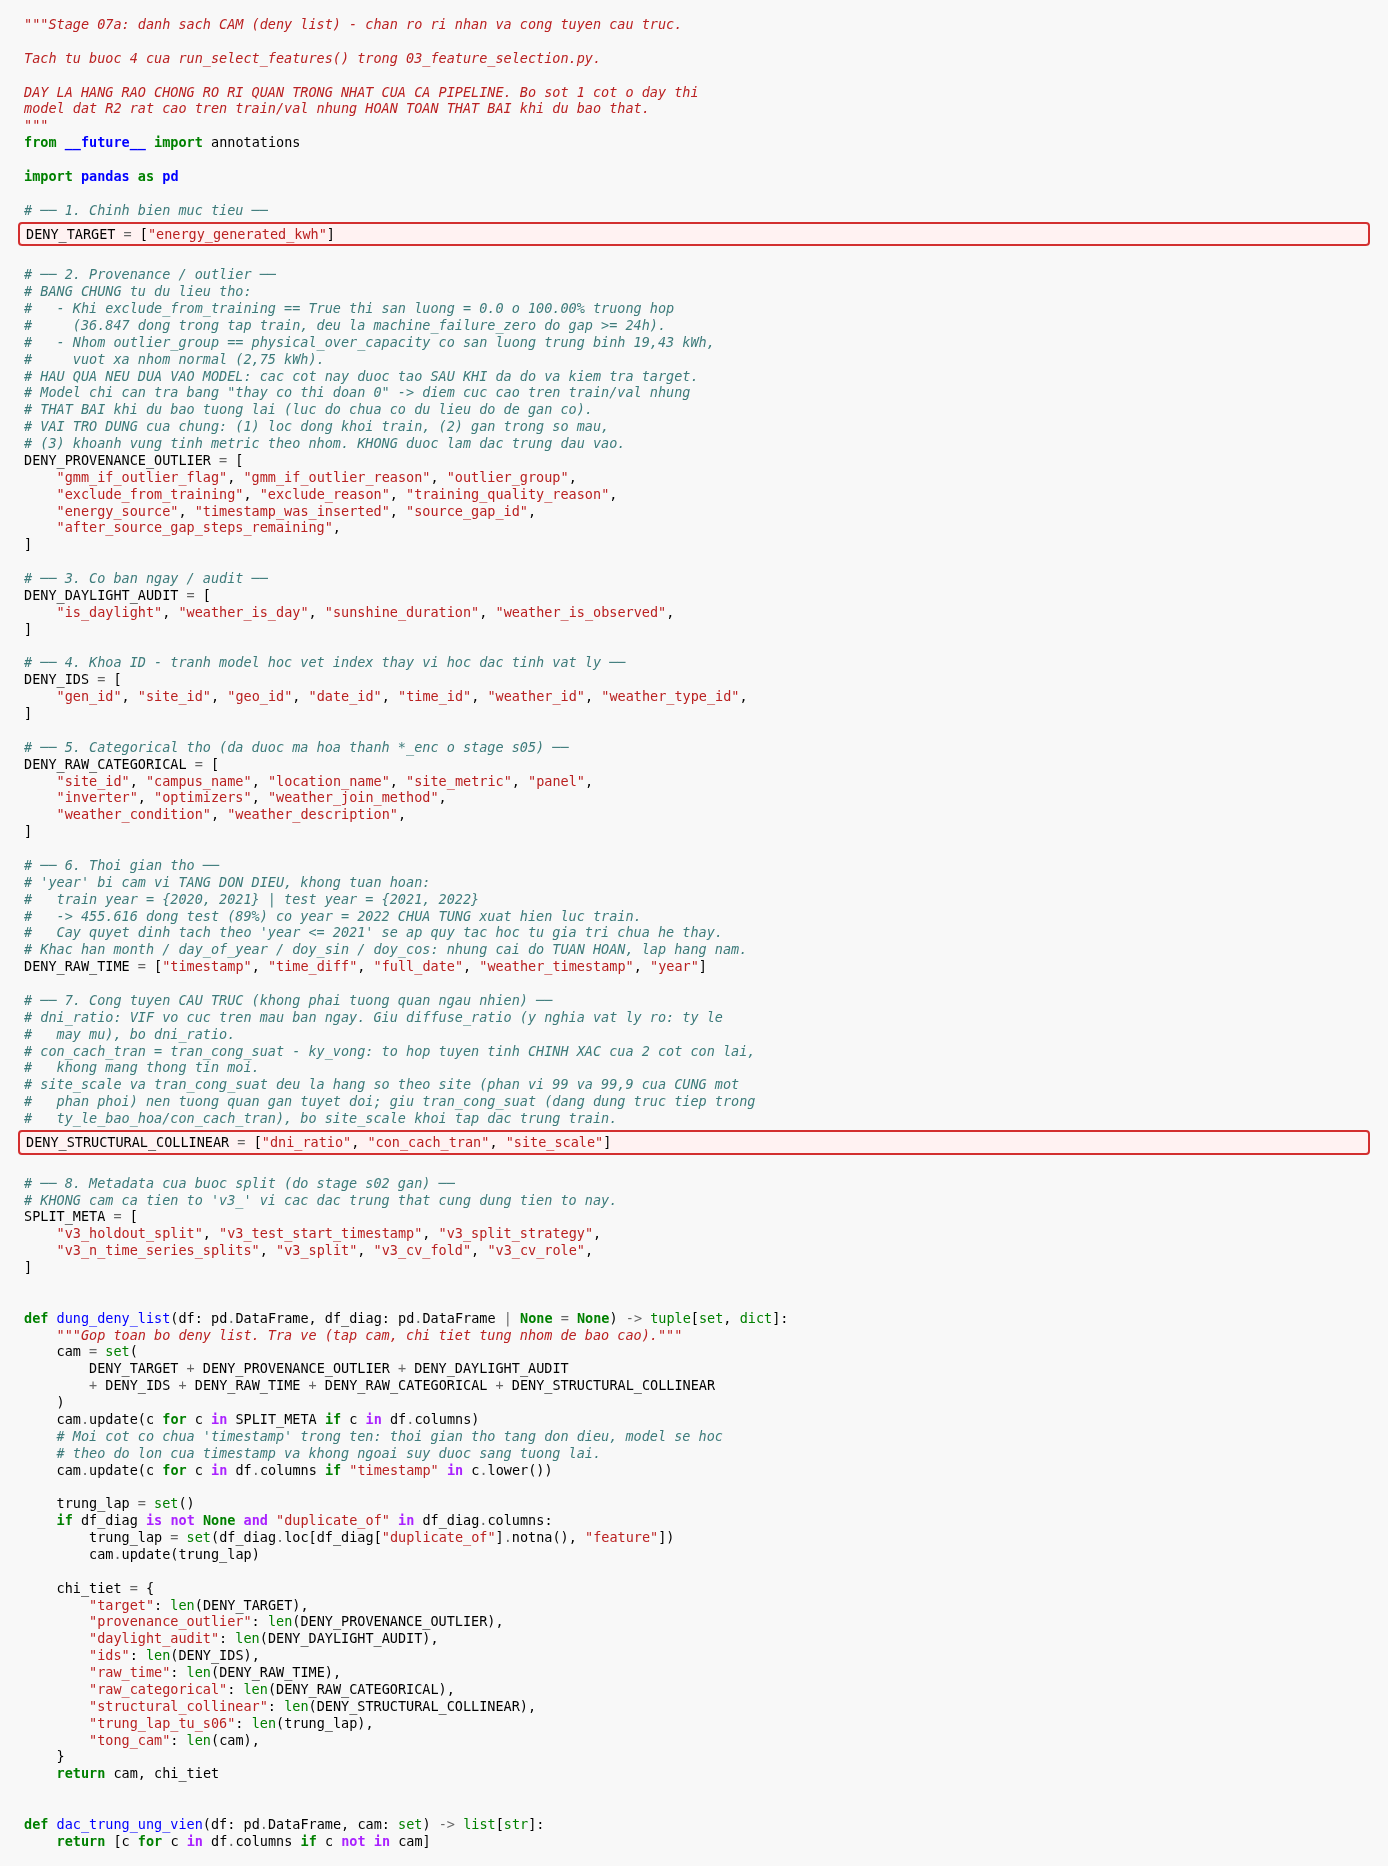
\includegraphics[width=0.95\textwidth]{images/code_pipeline_deny_list.png}
    \caption{Danh sách cấm đặc trưng trong Notebook \texttt{05\_select\_features.ipynb}, nhóm theo lý do: biến mục tiêu, nhãn nguồn gốc và nhãn bất thường, khoá định danh, biến phân loại thô, nhãn thời gian thô, và nhóm đồng tuyến cấu trúc.}
    \label{fig:code_deny_list}
\end{figure}

Trong chính sách Deny List của Notebook 05:
\begin{itemize}
    \item \textbf{Loại \texttt{lag\_1}:} Đặc trưng này không xuất hiện trong danh sách được chọn hiện tại; báo cáo không gán VIF hoặc mức cải thiện WAPE riêng khi chưa có thử nghiệm loại bỏ riêng tương ứng.
    \item \textbf{Giữ các chu kỳ được kiểm tra:} Notebook \texttt{03\_1\_features\_time.ipynb} sinh \texttt{lag\_4}, \texttt{lag\_96} và các cửa sổ trượt tương ứng; tệp kết quả 40 đặc trưng xác nhận \texttt{lag\_4}, \texttt{lag\_96} còn được dùng.
\end{itemize}

\section[VÍ DỤ TÍNH TOÁN THỦ CÔNG TỪNG BƯỚC TRẠM 1]{VÍ DỤ TÍNH TOÁN THỦ CÔNG TỪNG BƯỚC VỚI DỮ LIỆU TRẠM 1\\(WORKED HAND CALCULATION)}

Để minh họa cách tính các đại lượng trong pipeline, dưới đây là ví dụ tính toán thủ công trên bốn mốc thời gian của Trạm 1 (công suất lắp đặt $P_{\text{capacity}} = 51.15\text{ kWp}$) ngày 18/12/2021:

\begin{table}[H]
\centering
\caption{Dữ liệu thực tế và kết quả dự báo tại Trạm 1 (Site 1) khung giờ 11:00 -- 11:45}
\label{tab:worked_example_data}
\resizebox{\linewidth}{!}{%
\begin{tabular}{c c c c c c c}
\toprule
\textbf{Mốc Thời Gian} & \textbf{$y_{\text{true}}$ (kWh)} & \textbf{$\hat{y}_{\text{pred}}$ (kWh)} & \textbf{Góc $h$ ($^\circ$)} & \textbf{$\sin(h)$} & \textbf{$GHI_{\text{cs}}$ (W/m$^2$)} & \textbf{Temp ($^\circ$)} \\
\midrule
11:00 & 10.6875 & 9.5451 & 59.44 & 0.8611 & 1478.12 & 30.6 \\
11:15 & 14.8125 & 9.1445 & 62.33 & 0.8856 & 1522.98 & 30.6 \\
11:30 & 12.3125 & 9.0846 & 65.14 & 0.9074 & 1562.72 & 30.6 \\
11:45 & 10.2500 & 9.0575 & 67.85 & 0.9262 & 1597.19 & 30.6 \\
\bottomrule
\end{tabular}%
}
\end{table}

\subsection{Ví dụ 1: Tính toán thủ công Sản lượng nén cấp Giờ ($E_{\text{hourly}}$) và WAPE Khung Giờ}
\begin{enumerate}
    \item \textbf{Tổng sản lượng thực tế trong khung giờ ($E_{\text{actual, 1h}}$):}
    \begin{equation}
        E_{\text{actual, 1h}} = 10.6875 + 14.8125 + 12.3125 + 10.2500 = \mathbf{48.0625 \text{ kWh}}
    \end{equation}

    \item \textbf{Tổng sản lượng dự báo trong khung giờ ($E_{\text{pred, 1h}}$):}
    \begin{equation}
        E_{\text{pred, 1h}} = 9.5451 + 9.1445 + 9.0846 + 9.0575 = \mathbf{36.8317 \text{ kWh}}
    \end{equation}

    \item \textbf{Tổng sai số tuyệt đối các mốc ($\sum |e_i|$):}
    \begin{align}
        |e_1| &= |10.6875 - 9.5451| = 1.1424 \text{ kWh} \\
        |e_2| &= |14.8125 - 9.1445| = 5.6680 \text{ kWh} \\
        |e_3| &= |12.3125 - 9.0846| = 3.2279 \text{ kWh} \\
        |e_4| &= |10.2500 - 9.0575| = 1.1925 \text{ kWh} \\
        \sum_{i=1}^{4} |e_i| &= 1.1424 + 5.6680 + 3.2279 + 1.1925 = \mathbf{11.2308 \text{ kWh}}
    \end{align}

    \item \textbf{Tính toán thủ công chỉ số WAPE của khung giờ này:}
    \begin{equation}
        \text{WAPE}_{\text{1h}} = \frac{\sum_{i=1}^{4} |e_i|}{\sum_{i=1}^{4} y_i} \times 100\% = \frac{11.2308}{48.0625} \times 100\% = \mathbf{23.37\%}
    \end{equation}
\end{enumerate}

\subsection{Ví dụ 2: Tính toán thủ công Tỷ số Hiệu suất Trạm Phát (Performance Ratio - PR) tại Mốc 11:15}
Trạm 1 có công suất định mức $P_{\text{stc}} = 51.15 \text{ kWp}$. Tại mốc 11:15, sản lượng thực tế $E_{\text{15min}} = 14.8125 \text{ kWh}$, bức xạ mặt phẳng nghiêng ghi nhận $G_{poa} = 344.27 \text{ W/m}^2$.
\begin{equation}
    \text{PR} = \frac{E_{\text{actual}}}{P_{\text{stc}} \times \left(\frac{G_{poa}}{1000}\right) \times 0.25 \text{h}} = \frac{14.8125}{51.15 \times \left(\frac{344.27}{1000}\right) \times 0.25} = \frac{14.8125}{4.4024} = \mathbf{0.8413} \quad (\mathbf{84.13\%})
\end{equation}

\subsection{Ví dụ 3: Tính tay Huber Loss (\texorpdfstring{$\delta=0.9$}{delta=0.9}) vs MSE vs MAE tại Mốc 11:30}
Tại mốc 11:30, $y_{\text{true}} = 12.3125 \text{ kWh}$, $\hat{y}_{\text{pred}} = 9.0846 \text{ kWh}$. Sai số $e = y - \hat{y} = 3.2279 \text{ kWh}$.
\begin{enumerate}
    \item \textbf{Tính toán thủ công MSE Loss:} $L_{\text{MSE}} = \frac{1}{2} e^2 = \frac{1}{2} (3.2279)^2 = \mathbf{5.2096}$.
    \item \textbf{Tính toán thủ công MAE Loss:} $L_{\text{MAE}} = |e| = \mathbf{3.2279}$.
    \item \textbf{Tính toán thủ công Huber Loss ($\delta=0.9$):} $L_{\text{Huber}} = \delta |e| - \frac{1}{2}\delta^2 = 0.9 \times 3.2279 - 0.405 = \mathbf{2.5001}$.
\end{enumerate}

\subsection{Ví dụ 4: Tính Toán Thủ Công Chi Tiết Cho Cả 5 Nhóm Đặc Trưng Kỹ Thuật (Feature Groups)}
Tại thời điểm 11:15 ngày 18/12/2021 của Trạm 1, các đặc trưng được minh họa bằng phép tính từ dữ liệu đầu vào:

\begin{enumerate}
    \item \textbf{Nhóm 1 --- Lịch tuần hoàn Sin/Cos (Giờ: 11:15 $\Rightarrow \text{hour\_float} = 11.25$h, Ngày trong năm: 352):}
    \begin{align}
        \text{hour\_sin} &= \sin\left(\frac{2\pi \times 11.25}{24}\right) = \sin(168.75^\circ) = \mathbf{0.19509} \\
        \text{hour\_cos} &= \cos\left(\frac{2\pi \times 11.25}{24}\right) = \cos(168.75^\circ) = \mathbf{-0.98079} \\
        \text{day\_sin} &= \sin\left(\frac{2\pi \times 352}{365.25}\right) = \sin(346.79^\circ) = \mathbf{-0.2285}
    \end{align}

\item \textbf{Nhóm 2 --- Hình học Mặt trời}\\(Góc nâng $h = 62.33^\circ$, $GHI_{\text{rad}} = 354.5\text{ W/m}^2$),
    \begin{align}
        \text{sin\_elevation} &= \sin(62.33^\circ) = \mathbf{0.885635} \\
        K_t \ (\text{Clear-Sky Index}) &= \frac{GHI_{\text{raw}}}{GHI_{\text{clearsky}}} = \frac{354.5}{1522.98} = \mathbf{0.2328}
    \end{align}

    \item \textbf{Nhóm 3 --- Đặc trưng khí tượng (Nhiệt độ $T = 30.6^\circ\text{}$):}
    \begin{equation}
        T_{\text{Kelvin}} = 30.6 + 273.15 = \mathbf{303.75 \text{ K}}
    \end{equation}

    \item \textbf{Nhóm 4 --- Tương tác Khí tượng ($GHI = 354.5 \text{ W/m}^2$, $\text{cloud} = 12\%$, $lag_{96} = 20.3125 \text{ kWh}$):}
    \begin{align}
        \text{ghi\_temp\_ratio} &= \frac{GHI}{T_{\text{Kelvin}}} = \frac{354.5}{303.75} = \mathbf{1.1671 \text{ W/(m}^2\cdot\text{K)}} \\
        \text{cloud\_temp\_interaction} &= \text{cloud\_cover} \times T_{\text{Celsius}} = 12 \times 30.6 = \mathbf{367.2} \\
        \text{delta\_lag96} &= y_t - lag_{96} = 14.8125 - 20.3125 = \mathbf{-5.5000 \text{ kWh}}
    \end{align}

    \item \textbf{Nhóm 5 --- Rolling Features}\\
(4 mốc 15 phút vừa qua: $10.6875, 14.8125, 12.3125, 10.2500 \text{ kWh}$):
    \begin{align}
        \text{rolling\_mean\_4} &= \frac{10.6875 + 14.8125 + 12.3125 + 10.2500}{4} = \mathbf{12.0156 \text{ kWh}} \\
        \text{rolling\_std\_4} &= \sqrt{\frac{(10.6875-12.0156)^2 + \dots + (10.2500-12.0156)^2}{4 - 1}} = \mathbf{2.0650 \text{ kWh}}
    \end{align}
\end{enumerate}

\section[PHÂN TÍCH HÀM MẤT MÁT VÀ ĐIỀU HÓA]{PHÂN TÍCH HÀM MẤT MÁT VÀ ĐIỀU HÓA\\REGULARIZATION LOSS}

\subsection{So sánh lý thuyết toán học các hàm mất mát\\(MSE, MAE và Huber Loss)}
\begin{enumerate}
    \item \textbf{Mean Squared Error (MSE Loss):} $L_{\text{MSE}}(y, \hat{y}) = \frac{1}{2} (y - \hat{y})^2$.  
    \textit{\textbf{Nguồn sách giáo khoa tham khảo:} Hastie, Tibshirani, Friedman (2009), "The Elements of Statistical Learning: Data Mining, Inference, and Prediction".}

    \item \textbf{Mean Absolute Error (MAE Loss):} $L_{\text{MAE}}(y, \hat{y}) = |y - \hat{y}|$.  
    \textit{\textbf{Nguồn sách tham khảo:} Rob J. Hyndman, George Athanasopoulos (2018), "Forecasting: Principles and Practice", OTexts.}

    \item \textbf{Huber Loss ($\delta=0.9$):}
    $L_\delta(y, \hat{y}) = \begin{cases} \frac{1}{2}(y - \hat{y})^2 & \text{với } |y - \hat{y}| \le \delta \\ \delta |y - \hat{y}| - \frac{1}{2}\delta^2 & \text{với } |y - \hat{y}| > \delta \end{cases}$.  
    \textit{\textbf{Nguồn bài báo tham khảo:} Peter J. Huber (1964), "Robust Estimation of a Location Parameter," \textit{Annals of Mathematical Statistics}, 35(1), 73--101.}
\end{enumerate}

\begin{figure}[htbp]
    \centering
    \includegraphics[width=0.82\textwidth]{images/loss_functions_comparison.png}
    \caption{(Biểu đồ Lý thuyết) So sánh đồ thị các hàm mất mát MSE, MAE, Huber Loss ($\delta=0.9$) và Đạo hàm Gradient}
    \label{fig:loss_comparison}
\end{figure}
\textbf{Diễn giải Hình \ref{fig:loss_comparison}:} Huber Loss ($\delta=0.9$) có dạng bình phương khi sai số nhỏ ($|e| \le 0.9$) và dạng tuyến tính khi sai số lớn ($|e| > 0.9$). Đây là hình minh họa lý thuyết, không phải đường cong tối ưu của một trial cụ thể. Việc lựa chọn hàm mất mát cuối cùng được căn cứ vào WAPE validation trình bày ở Bảng \ref{tab:benchmark_loss_val}.

Các đường cong huấn luyện thực tế của MAE, Huber và MSE tại H1/H4 được trình bày ở các Hình \ref{fig:loss_curve_mae_h1}--\ref{fig:loss_curve_mse_h4}. Đây là chẩn đoán quá trình boosting; kết quả chính và quyết định hàm mất mát được lấy từ tệp validation của \texttt{06\_4\_validate\_model\_selection.ipynb}.

\subsection{Hàm Huấn Luyện Mô Hình Chính (Model Training Core)}

\begin{figure}[htbp]
    \centering
    \includegraphics[width=0.95\textwidth]{images/code_notebook_fit_an_toan.png}
    \caption{Các hàm hỗ trợ huấn luyện LightGBM: cấu hình thiết bị tính toán và khởi tạo \texttt{LGBMRegressor}; khi GPU không khả dụng, pipeline sử dụng CPU với cùng thư viện LightGBM.}
    \label{fig:code_fit_an_toan}
\end{figure}

\subsection[Tính Bất Định GPU trong LightGBM]{Giải Thích Tính Bất Định GPU (Non-Deterministic) Khi Huấn Luyện LightGBM: Khác Biệt Kết Quả Giữa Jupyter Notebook và File Script (.py)}

\begin{figure}[htbp]
    \centering
    \includegraphics[width=0.92\textwidth]{images/lightgbm_gpu_nondeterministic_docs.png}
    \caption{Trích đoạn Tài liệu Kỹ thuật Chính thức từ Microsoft LightGBM (ReadTheDocs): Quy định tham số \texttt{deterministic} chỉ áp dụng cho CPU và Cảnh báo Tính Không Xác Định (\textit{Non-Deterministic}) Khi Huấn Luyện Trên GPU}
    \label{fig:lightgbm_gpu_nondeterministic}
\end{figure}

\textbf{Ý nghĩa Kỹ thuật \& Giải thích Sự Khác biệt Kết quả (Hình \ref{fig:lightgbm_gpu_nondeterministic}):}
\begin{enumerate}
    \item \textbf{Tham số \texttt{deterministic}:} Theo tài liệu LightGBM, tham số \texttt{deterministic=true} chỉ áp dụng cho thiết bị CPU. Với GPU (\texttt{device\_type='gpu'} hoặc \texttt{'cuda'}), kết quả có thể khác biệt nhỏ giữa các lần huấn luyện do phép tính song song.
    \item \textbf{Nguyên nhân Tính Bất Định trên GPU:} Quá trình tổng hợp số thực phẩy động (\textit{floating-point reduction}) trong các hạt nhân tính toán CUDA/OpenCL diễn ra theo thứ tự luồng song song ngẫu nhiên. Khi cộng các số thực phẩy động theo các thứ tự luồng khác nhau, sai số làm tròn vi mô ở các chữ số thập phân cuối ($10^{-6} \sim 10^{-8}$) sẽ được tích lũy và lan truyền qua hàng ngàn cây quyết định.
    \item \textbf{Giải thích Khác biệt giữa Jupyter Notebook và File Script (\texttt{.py}):} 
    Khi chạy trong Jupyter Notebook hoặc bằng tệp \texttt{.py}, môi trường thực thi và thứ tự thực hiện các phép tính song song có thể khác nhau. Vì vậy, với huấn luyện trên GPU, các chỉ số như WAPE hoặc MAE có thể sai khác nhẹ ở các chữ số thập phân cuối dù cùng sử dụng một giá trị hạt giống ngẫu nhiên (\texttt{random\_state = 42} hoặc \texttt{seed = 42}).
\end{enumerate}

\subsection[Hàm Phạt Điều Hóa Regularization]{Hàm Phạt Điều Hóa Regularization trong LightGBM\\(L1 vs L2 vs Elastic Net)~\cite{zou2005elasticnet}}
Để hạn chế quá khớp trên tập huấn luyện, hàm mục tiêu của LightGBM có thể kết hợp các thành phần phạt $L_1$ (\texttt{reg\_alpha}) và $L_2$ (\texttt{reg\_lambda}) trên trọng số lá cây $w_j$:

\begin{equation}
    \mathcal{O}^{(t)} = \sum_{i=1}^{n} L\left(y_i, \hat{y}_i^{(t-1)} + f_t(x_i)\right) + \Omega_{\text{ElasticNet}}(f_t)
\end{equation}

\begin{equation}
    \Omega_{\text{ElasticNet}}(f_t) = \gamma T + \alpha \sum_{j=1}^{T} |w_j| + \frac{1}{2} \lambda \sum_{j=1}^{T} w_j^2
\end{equation}
\textit{\textbf{Nguồn bài báo tham khảo gốc về Elastic Net:} Hui Zou \& Trevor Hastie (2005), "Regularization and Variable Selection via the Elastic Net", Journal of the Royal Statistical Society: Series B (Statistical Methodology), 67(2), 301-320.}

\begin{enumerate}
    \item \textbf{Phạt $L_1$ Lasso Regularization ($\alpha = \text{\texttt{reg\_alpha}}$):} Về mặt hình học tổng quát (hồi quy tuyến tính), tạo đường giới hạn hình kim cương ($\diamond$), có thể ép hệ số về đúng $0$. Trong LightGBM, phạt $L_1$ tác động lên \textbf{trọng số lá cây}, làm giảm độ lớn trọng số các lá ít đóng góp — không phải cơ chế feature-selection cứng như Lasso tuyến tính.
    \item \textbf{Phạt $L_2$ Ridge Regularization ($\lambda = \text{\texttt{reg\_lambda}}$):} Về mặt hình học tổng quát, tạo đường giới hạn hình tròn ($\bigcirc$), thu nhỏ liên tục các hệ số (\textit{weight shrinkage}). Trong LightGBM, phạt $L_2$ giúp làm mượt trọng số lá cây, gián tiếp giảm overfitting khi có đặc trưng tương quan cao — không xử lý VIF trực tiếp như Ridge tuyến tính.
    \item \textbf{Phạt Elastic Net Combined Regularization ($\alpha > 0, \lambda > 0$):} Tạo đường giới hạn bo tròn góc kim cương. Kết hợp ưu điểm của cả hai: vừa duy trì tính thưa (\textit{sparsity}) của $L_1$, vừa có hiệu ứng nhóm (\textit{grouping effect}) của $L_2$ để xử lý các nhóm đặc trưng thời tiết cùng biến động mạnh.
\end{enumerate}

\begin{figure}[htbp]
    \centering
    \includegraphics[width=0.82\textwidth]{images/regularization_loss_diagram.png}
    \caption{(Sơ đồ Lý thuyết, minh họa trực giác chung cho hồi quy tuyến tính có điều hóa) Đường biên giới hạn điều hóa L1 Regularization (Lasso), L2 Regularization (Ridge) và Elastic Net}
    \label{fig:reg_diagram}
\end{figure}
\textbf{Diễn giải Hình \ref{fig:reg_diagram}:} Hình minh họa trực giác chung về điều hóa $L_1$/$L_2$ trong hồi quy tuyến tính. Với LightGBM, hai thành phần phạt tác động lên trọng số lá cây $w_j$, không phải hệ số của từng đặc trưng; vì vậy chúng không tương đương với cơ chế chọn biến hoặc xử lý VIF trực tiếp trong hồi quy tuyến tính.

\section[DANH SÁCH BÀI BÁO KHOA HỌC QUỐC TẾ THAM KHẢO]{DANH SÁCH BÀI BÁO KHOA HỌC QUỐC TẾ THAM KHẢO\\(CITED PAPERS IN NOTEBOOKS)}

\begin{enumerate}
    \item \textbf{NeurIPS 2019 (Vincent Le Guen \& Nicolas Thome):} \textit{"Shape and Time Distortion Loss for Training Deep Time Series Forecasting Models (DILATE)"}, pp. 4191--4203. Link: \url{https://arxiv.org/abs/1909.09020}
    \textbf{Liên quan đến dự án:} lý do khái niệm cho việc phải kiểm tra riêng \textbf{độ trễ pha} bên cạnh WAPE — DILATE là ví dụ hàm mất mát học thuật tách rời sai lệch hình dạng và sai lệch thời gian. Notebook \texttt{09\_kiem\_chung\_tre\_pha.ipynb} hiện ghi nhận trung vị độ lệch đỉnh cục bộ khoảng $+15$ phút, nên báo cáo không tuyên bố độ trễ bằng 0; pipeline không huấn luyện trực tiếp bằng DILATE.
    \item \textbf{ArXiv 2024 (Bailey et al.):} \textit{"Temporal and Spatial Downscaling for Solar Radiation Forecasting"}. Link: \url{https://arxiv.org/pdf/2405.11046}
    \textbf{Liên quan đến dự án:} cùng chủ đề downscale bức xạ theo thời gian/không gian mà dự án giải quyết ở bước tái tạo GHI 15 phút từ dữ liệu Open-Meteo 1 giờ.
    \item \textbf{NREL/CP-5500-60142 (J. Zhang, B.-M. Hodge, A. Florita et al., 2013):} \textit{"Metrics for Evaluating the Accuracy of Solar Power Forecasting"}. Link: \url{https://www.nrel.gov/docs/fy14osti/60142.pdf} (OSTI ID: 1114086: \url{https://www.osti.gov/biblio/1114086})
    \textbf{Liên quan đến dự án:} cơ sở triết lý đánh giá đa chỉ số (RMSE/MBE/MAE so với baseline tham chiếu) mà dự án áp dụng khi so sánh mô hình LightGBM với Prophet baseline; công thức WAPE cụ thể dự án dùng lấy từ bài PIN 2025 riêng (Hình \ref{fig:paper_pin_wape_table}).
\end{enumerate}

\begin{figure}[htbp]
    \centering
    \includegraphics[width=0.85\textwidth]{images/paper_leguen_dilate_2019_khung.png}
    \caption{Ảnh chụp trang đầu của bài báo Le Guen \& Thome (2019)~\cite{leguen2019}, NeurIPS, arXiv:1909.09020. Abstract nêu DILATE tách sai lệch \textit{shape} và \textit{temporal change} để đánh giá/huấn luyện dự báo chuỗi thời gian. Dự án lấy ngữ cảnh cần kiểm tra sai lệch thời gian của đỉnh và ramp; pipeline hiện tại không tuyên bố đã huấn luyện trực tiếp bằng DILATE loss.}
    \label{fig:paper_dilate}
\end{figure}

\begin{figure}[htbp]
    \centering
    \includegraphics[width=0.85\textwidth]{images/paper_zhang2015_realmetrics.png}
    \caption{Ảnh chụp trang đầu của bài báo Zhang et al. (2015)~\cite{zhang2015metrics}, \textit{Solar Energy} 111, 157--175, DOI: 10.1016/j.solener.2014.10.016. Abstract nêu một bộ metrics tổng quát và khung đánh giá độ nhạy cho dự báo điện mặt trời. Dự án lấy ngữ cảnh đánh giá đa chiều; WAPE daylight và cách tính Skill Score theo baseline cụ thể là định nghĩa thực nghiệm của dự án.}
    \label{fig:paper_zhang2015real}
\end{figure}

\section[HÌNH ẢNH VÀ ĐỒ THỊ KIỂM CHỨNG]{HÌNH ẢNH VÀ ĐỒ THỊ KIỂM CHỨNG\\TỪ NGUỒN NOTEBOOKS (\texttt{notebooks/forcasting\_v3\_energy/})}

\begin{figure}[htbp]
    \centering
    \includegraphics[width=0.80\textwidth]{images/notebook_acf_pacf.png}
    \caption{(Trích xuất từ Notebook \texttt{v1\_AF\_PAF.ipynb}) Đồ thị tự tương quan AF/PAF chuỗi thời gian sản lượng}
    \label{fig:nb_acf_pacf}
\end{figure}

\begin{figure}[htbp]
    \centering
    \includegraphics[width=0.80\textwidth]{images/notebook_correlation_heatmap.png}
    \caption{(Trích xuất từ Notebook \texttt{v2\_\_correlation\_heatmap.ipynb}) Ma trận tương quan Spearman ban ngày}
    \label{fig:nb_heatmap}
\end{figure}

\begin{figure}[htbp]
    \centering
    \includegraphics[width=0.80\textwidth]{images/notebook_vif_diagnostics.png}
    \caption{(Trích xuất từ Notebook \texttt{04\_vif\_diagnostics.ipynb}) Biểu đồ chẩn đoán đa cộng tuyến VIF \& Chính sách Deny List}
    \label{fig:nb_vif}
\end{figure}

\begin{figure}[htbp]
    \centering
    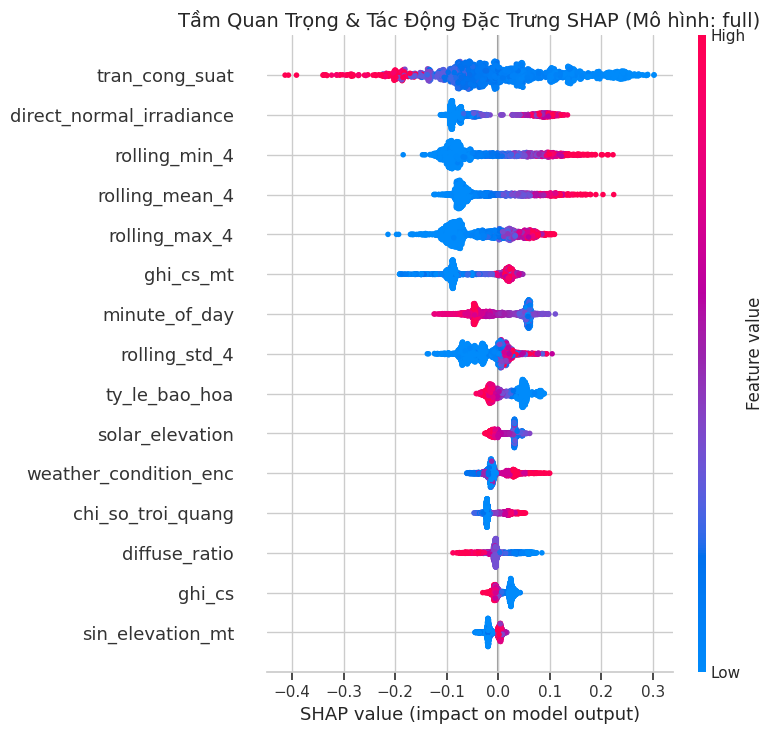
\includegraphics[width=0.80\textwidth]{images/notebook_shap_beeswarm.png}
    \caption{(Trích xuất từ Notebook \texttt{08\_explainable\_ai.ipynb}) Đồ thị SHAP Summary Beeswarm Tác động Toàn cục của Các Đặc trưng}
    \label{fig:nb_shap_beeswarm}
\end{figure}

\begin{figure}[htbp]
    \centering
    \includegraphics[width=0.80\textwidth]{images/notebook_shap_waterfall.png}
    \caption{(Trích xuất từ Notebook \texttt{08\_explainable\_ai.ipynb}) Đồ thị SHAP Waterfall Phân Tích Chi Tiết 1 Mốc Dự báo Cụ thể}
    \label{fig:nb_shap_waterfall}
\end{figure}

\begin{figure}[htbp]
    \centering
    \includegraphics[width=0.80\textwidth]{images/notebook_feature_importance.png}
    \caption{(Trích xuất từ Notebook \texttt{06\_1\_train\_mae.ipynb}) Xếp hạng đặc trưng Feature Importance (Gain) trong LightGBM}
    \label{fig:nb_imp}
\end{figure}

\begin{figure}[htbp]
    \centering
    \includegraphics[width=0.80\textwidth]{images/notebook_toan_canh_1_tuan.png}
    \caption{Đồ thị chuỗi thời gian một tuần trên tập kiểm thử giữ lại, trích xuất từ Notebook \texttt{06\_1\_train\_mae.ipynb}.}
    \label{fig:nb_1tuan}
\end{figure}

\begin{figure}[htbp]
    \centering
    \includegraphics[width=0.80\textwidth]{images/notebook_zoom_quanh_dinh.png}
    \caption{(Trích xuất từ Notebook \texttt{06\_1\_train\_mae.ipynb}) Đồ thị zoom chi tiết mốc đỉnh sản lượng thực tế và dự báo không bị lệch pha}
    \label{fig:nb_zoom}
\end{figure}

\section[BẢNG TỔNG HỢP KẾT QUẢ BENCHMARK]{BẢNG TỔNG HỢP KẾT QUẢ BENCHMARK\\TRÊN TẬP KIỂM THỬ GIỮ LẠI}

\subsection[Mô Hình Baseline Chính Thức: Facebook Prophet]{Xác Định Mô Hình Baseline Chính Thức của Dự Án: Facebook Prophet}
Nghiên cứu sử dụng Facebook Prophet làm mô hình đối chứng chính thức. Prophet là mô hình chuỗi thời gian được công nhận rộng rãi, và quan trọng hơn, nó đại diện cho đúng nhóm phương pháp mà nghiên cứu này muốn đối chiếu: dự báo chỉ dựa trên tính chu kỳ của lịch sử sản lượng, không sử dụng thông tin khí tượng. Chênh lệch giữa hai mô hình vì thế đo trực tiếp phần đóng góp của khối đặc trưng khí tượng:

\begin{center}
\fbox{
\begin{minipage}{0.95\linewidth}
\textbf{Đặc điểm của Baseline Chính thức Prophet (Notebook 06\_0b):}
\begin{itemize}
    \item \textbf{Nguyên lý:} Mô hình chuỗi thời gian cộng tính (\textit{additive time-series model}) học thành phần xu hướng và chu kỳ ngày, tuần riêng cho từng trạm.
    \item \textbf{Phạm vi dữ liệu:} Không sử dụng các đặc trưng khí tượng như $GHI$, nhiệt độ, độ mây hoặc góc nâng Mặt Trời.
    \item \textbf{Vai trò đối chứng:} Đo lường khả năng dự báo của các phương pháp thống kê truyền thống khi chỉ dựa vào lịch sử sản lượng thuần túy.
\end{itemize}
\end{minipage}
}
\end{center}

\subsection[Thí Nghiệm Chọn Hàm Mất Mát Trên Tập Validation]{Thí Nghiệm So Sánh 3 Hàm Mất Mát (MSE / MAE / Huber) Trên Tập Validation}
Ba hàm mất mát được tối ưu hóa độc lập bằng Optuna TPE, với $20$ lần thử cho mỗi hàm mất mát và mỗi tầm dự báo trong các Notebook \texttt{06\_1}, \texttt{06\_2}, \texttt{06\_3}. Kết quả được đối sánh trên tập validation giữ lại bên trong Development, chỉ gồm các dòng ban ngày đo thật:

\begin{figure}[htbp]
    \centering
    \includegraphics[width=0.95\textwidth]{images/code_notebook_optuna_tune_h4.png}
    \caption{Quy trình tối ưu siêu tham số bằng Optuna. Không gian tìm kiếm gồm tám siêu tham số (bổ sung \texttt{alpha} với Huber); mỗi cấu hình được đánh giá bằng \emph{pooled WAPE} trên năm fold mở rộng. Kết quả được lưu trong \texttt{best\_params.json} để tái sử dụng ở bước huấn luyện.}
    \label{fig:code_optuna_h4}
\end{figure}

\begin{table}[H]
\centering
\caption{Kết quả trên tập validation giữ lại bên trong Development, chỉ gồm các dòng ban ngày đo thật, giữa ba hàm mất mát. Số liệu trích từ \texttt{data/model/v3/07\_final\_test/val\_model\_selection\_check.json}; $n=220.807$ tại H1 và $n=220.687$ tại H4. \textbf{In đậm} là WAPE thấp nhất theo từng tầm dự báo và là tiêu chí chọn hàm mất mát.}
\label{tab:benchmark_loss_val}
\resizebox{\linewidth}{!}{%
\begin{tabular}{l c c c c c}
\toprule
\textbf{Hàm loss} & \textbf{WAPE (\%) $\downarrow$} & \textbf{RMSE (kWh) $\downarrow$} & \textbf{MAE (kWh) $\downarrow$} & \textbf{R² $\uparrow$} & \textbf{n} \\
\midrule
\multicolumn{6}{l}{\textbf{\textit{Horizon H1 (T+15 phút):}}} \\
MSE Loss & 21,6301\% & 3,9099 & 1,6783 & 0,9019 & 220.807 \\
\textbf{MAE Loss (được chọn)} & \textbf{21,0302\%} & 3,9567 & \textbf{1,6317} & 0,8996 & 220.807 \\
Huber Loss & 21,4990\% & \textbf{3,8844} & 1,6681 & \textbf{0,9032} & 220.807 \\
\midrule
\multicolumn{6}{l}{\textbf{\textit{Horizon H4 (T+60 phút / 1 giờ tới):}}} \\
MSE Loss & 25,6407\% & \textbf{4,4194} & 1,9702 & \textbf{0,8762} & 220.687 \\
\textbf{MAE Loss (được chọn)} & \textbf{25,2243\%} & 4,4527 & \textbf{1,9382} & 0,8743 & 220.687 \\
Huber Loss & 25,7314\% & 4,4211 & 1,9771 & 0,8761 & 220.687 \\
\bottomrule
\end{tabular}%
}
\end{table}

Theo đúng tiêu chí WAPE đã định trước, MAE được chọn cho cả H1 và H4. Huber có RMSE/$R^2$ tốt hơn ở một số ô nhưng không thắng tiêu chí chọn; Test niêm phong chỉ được mở sau khi quyết định này đã được ghi nhận. Validation ở đây là tập giữ lại trong Development, không phải một tập Test độc lập.

\begin{figure}[htbp]
    \centering
    \includegraphics[width=0.88\textwidth]{images/paper_nrel_zhang_2013_metrics_cropped_khung.png}
    \caption{Trích đoạn thật từ Zhang et al. (2013)~\cite{zhang2013nrelmetrics}, NREL/CP-5500-60142. Phần mở đầu của bài báo nêu các thước đo RMSE, MBE và MAE, đồng thời lập luận cần một bộ chỉ số để đánh giá dự báo trong nhiều bối cảnh. Dự án kế thừa ngữ cảnh đánh giá đa chỉ số; WAPE ban ngày và công thức Skill Score với mô hình đối chứng cụ thể được nhóm định nghĩa và kiểm nghiệm riêng.}
    \label{fig:paper_nrel_zhang_2013}
\end{figure}

\subsection[Bảng Tổng Hợp Kết Quả Benchmark]{Bảng Tổng Hợp Kết Quả Benchmark Đánh Giá Mô Hình}
Bảng \ref{tab:benchmark_all} trình bày kết quả trên tập Test niêm phong, gồm 486.120 quan sát tại H1 và 486.000 quan sát tại H4. Số liệu được trích trực tiếp từ \texttt{data/model/v3/07\_final\_test/h1/metrics\_overall.json}, \texttt{h4/metrics\_overall.json} và \texttt{08\_baseline\_prophet\_test/prophet\_test\_summary.json}; các Notebook nguồn tương ứng là \texttt{07\_final\_test.ipynb} và \texttt{06\_0b\_baseline\_prophet.ipynb}.

\begin{table}[H]
\centering
\caption{Kết quả benchmark của các mô hình. Số in đậm thể hiện kết quả tốt nhất trong từng cột.}
\label{tab:benchmark_all}
\label{tab:benchmark_summary}
\label{tab:benchmark_test}
\resizebox{\linewidth}{!}{%
\begin{tabular}{l l c c c c c}
\toprule
\textbf{Phương Pháp / Mô Hình} & \textbf{Tầm Dự Báo} & \textbf{WAPE (\%) $\downarrow$} & \textbf{RMSE (kWh) $\downarrow$} & \textbf{MAE (kWh) $\downarrow$} & \textbf{R² $\uparrow$} & \textbf{Số quan sát} \\
\midrule
\multicolumn{7}{l}{\textbf{\textit{Mô hình đề xuất --- LightGBM MAE, đo trên tập Test niêm phong:}}} \\
\textbf{LightGBM MAE (toàn thời gian)} & H1 (T+15m) & \textbf{17,22\%} & 2,4078 & 0,6773 & 0,9397 & 486.120 \\
\textbf{LightGBM MAE (ban ngày, đo thật)} & H1 (T+15m) & \textbf{17,82\%} & 3,4263 & 1,3399 & 0,9243 & 229.751 \\
\textbf{LightGBM MAE (toàn thời gian)} & H4 (T+60m) & \textbf{21,34\%} & 2,8116 & 0,8389 & 0,9177 & 486.000 \\
\textbf{LightGBM MAE (ban ngày, đo thật)} & H4 (T+60m) & \textbf{21,45\%} & 3,9673 & 1,5984 & 0,8993 & 229.751 \\
\midrule
\multicolumn{7}{l}{\textbf{\textit{Đối chứng Facebook Prophet --- hai mô hình đánh giá trên cùng một tập dữ liệu:}}} \\
Facebook Prophet (không đặc trưng khí tượng) & H1 (T+15m) & 36,31\% & 5,5297 & 2,7707 & 0,8036 & 220.114 \\
\textbf{LightGBM MAE (cùng phạm vi)} & H1 (T+15m) & \textbf{17,75\%} & \textbf{3,2918} & \textbf{1,3543} & \textbf{0,9304} & 220.114 \\
Facebook Prophet (không đặc trưng khí tượng) & H4 (T+60m) & 36,15\% & 5,6783 & 2,8918 & 0,7997 & 202.908 \\
\textbf{LightGBM MAE (cùng phạm vi)} & H4 (T+60m) & \textbf{21,78\%} & \textbf{3,9489} & \textbf{1,7420} & \textbf{0,9031} & 202.908 \\
\bottomrule
\end{tabular}%
}
\end{table}
\small{\textit{Forecast Skill Score suy ra từ khối đối chứng: $\text{SS} = +51{,}12\%$ tại H1 và $+39{,}76\%$ tại H4. Khối đối chứng dùng phạm vi chặt hơn khối trên --- ngoài điều kiện ban ngày và giá trị tại $T$ là số đo thật, còn yêu cầu nhãn tại $T+h$ cũng là số đo thật --- nên số quan sát nhỏ hơn và WAPE của mô hình tăng nhẹ so với khối trên. Đây là chênh lệch do phạm vi đánh giá, không phải do hai lần huấn luyện khác nhau.}}

\begin{center}
\fbox{
\begin{minipage}{0.95\linewidth}
\textbf{Thảo luận kết quả định lượng:}
\begin{enumerate}
    \item \textbf{So sánh với Prophet:} Trên phạm vi đánh giá chung của hai mô hình (220.114 quan sát H1, cả giá trị tại $T$ lẫn nhãn tại $T+h$ đều là số đo thật), LightGBM MAE đạt WAPE \textbf{17,75\%} còn Prophet đạt \textbf{36,31\%}, tương ứng $\text{SS} = \mathbf{+51{,}12\%}$. Tại H4, hai WAPE tương ứng là $21{,}78\%$ và $36{,}15\%$, với $\text{SS} = \mathbf{+39{,}76\%}$.
    \item \textbf{Đánh giá độ trễ pha:} Notebook \texttt{09\_kiem\_chung\_tre\_pha.ipynb} ghi nhận trung vị độ lệch đỉnh cục bộ khoảng $+15$ phút, 32/40 site có trung vị dương. Đây là kiểm tra bổ sung, không phải một chỉ số WAPE và không đồng nghĩa mọi đỉnh sản lượng đều trùng chính xác.
\end{enumerate}
\end{minipage}
}
\end{center}

\fi

\section[EXECUTIVE BI DASHBOARD]{TRỰC QUAN HÓA TRÊN\\EXECUTIVE BI DASHBOARD\\(PHÂN TÍCH GIAO DIỆN \& 17 BIỂU ĐỒ)}

\subsection[Tổng Quan Executive BI Dashboard]{Tổng Quan Hệ Thống Executive BI Dashboard\\(Streamlit Web App)}
Dashboard tương tác được phát triển bằng Streamlit để hỗ trợ xem kết quả dự báo, sai số và giải thích mô hình. Giao diện tổ chức thông tin theo thứ tự từ chỉ số tổng quan đến biểu đồ chi tiết.

Dashboard gồm ba trang, tích hợp các bộ lọc dữ liệu theo trạm, thời gian và nguồn mô hình; các trang cung cấp các biểu đồ phục vụ phân tích kết quả:
\begin{enumerate}
    \item \textbf{Trang 1 — Chuỗi Thời Gian \& So Sánh Baseline (\texttt{1\_TimeSeries.py}):} Giám sát sai số thực tế và dự báo, xếp hạng 42 trạm, phân bố dư thừa và đối sánh với Prophet Baseline (gồm 6 biểu đồ).
    \item \textbf{Trang 2 — Phân Tích Minh Bạch AI bằng SHAP (\texttt{2\_SHAP.py}):} Giải thích đóng góp đặc trưng ở quy mô toàn cục (Global) lẫn dự báo cục bộ (Local) (gồm 5 biểu đồ dashboard + 2 đồ thị notebook).
    \item \textbf{Trang 3 — Dự Báo Tới \& What-if (\texttt{3\_Du\_Bao.py}):} Gọi API Open-Meteo theo toạ độ thật của trạm, dự báo đệ quy tới 14 ngày và cho phép phân tích độ nhạy theo bức xạ, nhiệt độ, độ mây, quy mô hệ thống.
\end{enumerate}

\begin{figure}[htbp]
    \centering
    \includegraphics[width=0.82\textwidth]{images/dashboard_overview.png}
    \caption{Hình 9.1 (Giao diện thực tế từ Streamlit App): Tổng quan Giao diện Executive BI Dashboard trên Nền tảng Web Streamlit}
    \label{fig:st_overview}
\end{figure}

\begin{figure}[htbp]
    \centering
    \includegraphics[width=0.82\textwidth]{images/dashboard_full_page.png}
    \caption{Hình 9.2 (Giao diện thực tế từ Streamlit App): Màn hình Chi tiết Toàn trang Executive BI Dashboard}
    \label{fig:st_full_page}
\end{figure}

% =============================================================
\subsection[Trang 1: Giám Sát Chuỗi Thời Gian]{Trang Dashboard 1: Giám Sát Chuỗi Thời Gian\\\& Phân Tích Dư Thừa (\texttt{1\_TimeSeries.py})}

\begin{center}
\fbox{
\begin{minipage}{0.95\linewidth}
\textbf{Vai trò của Trang 1:}
Trang 1 cung cấp các bộ lọc theo trạm, khoảng thời gian và nguồn dữ liệu để người dùng xem chi tiết chuỗi dự báo và sai số.
\end{minipage}
}
\end{center}

\begin{figure}[htbp]
    \centering
    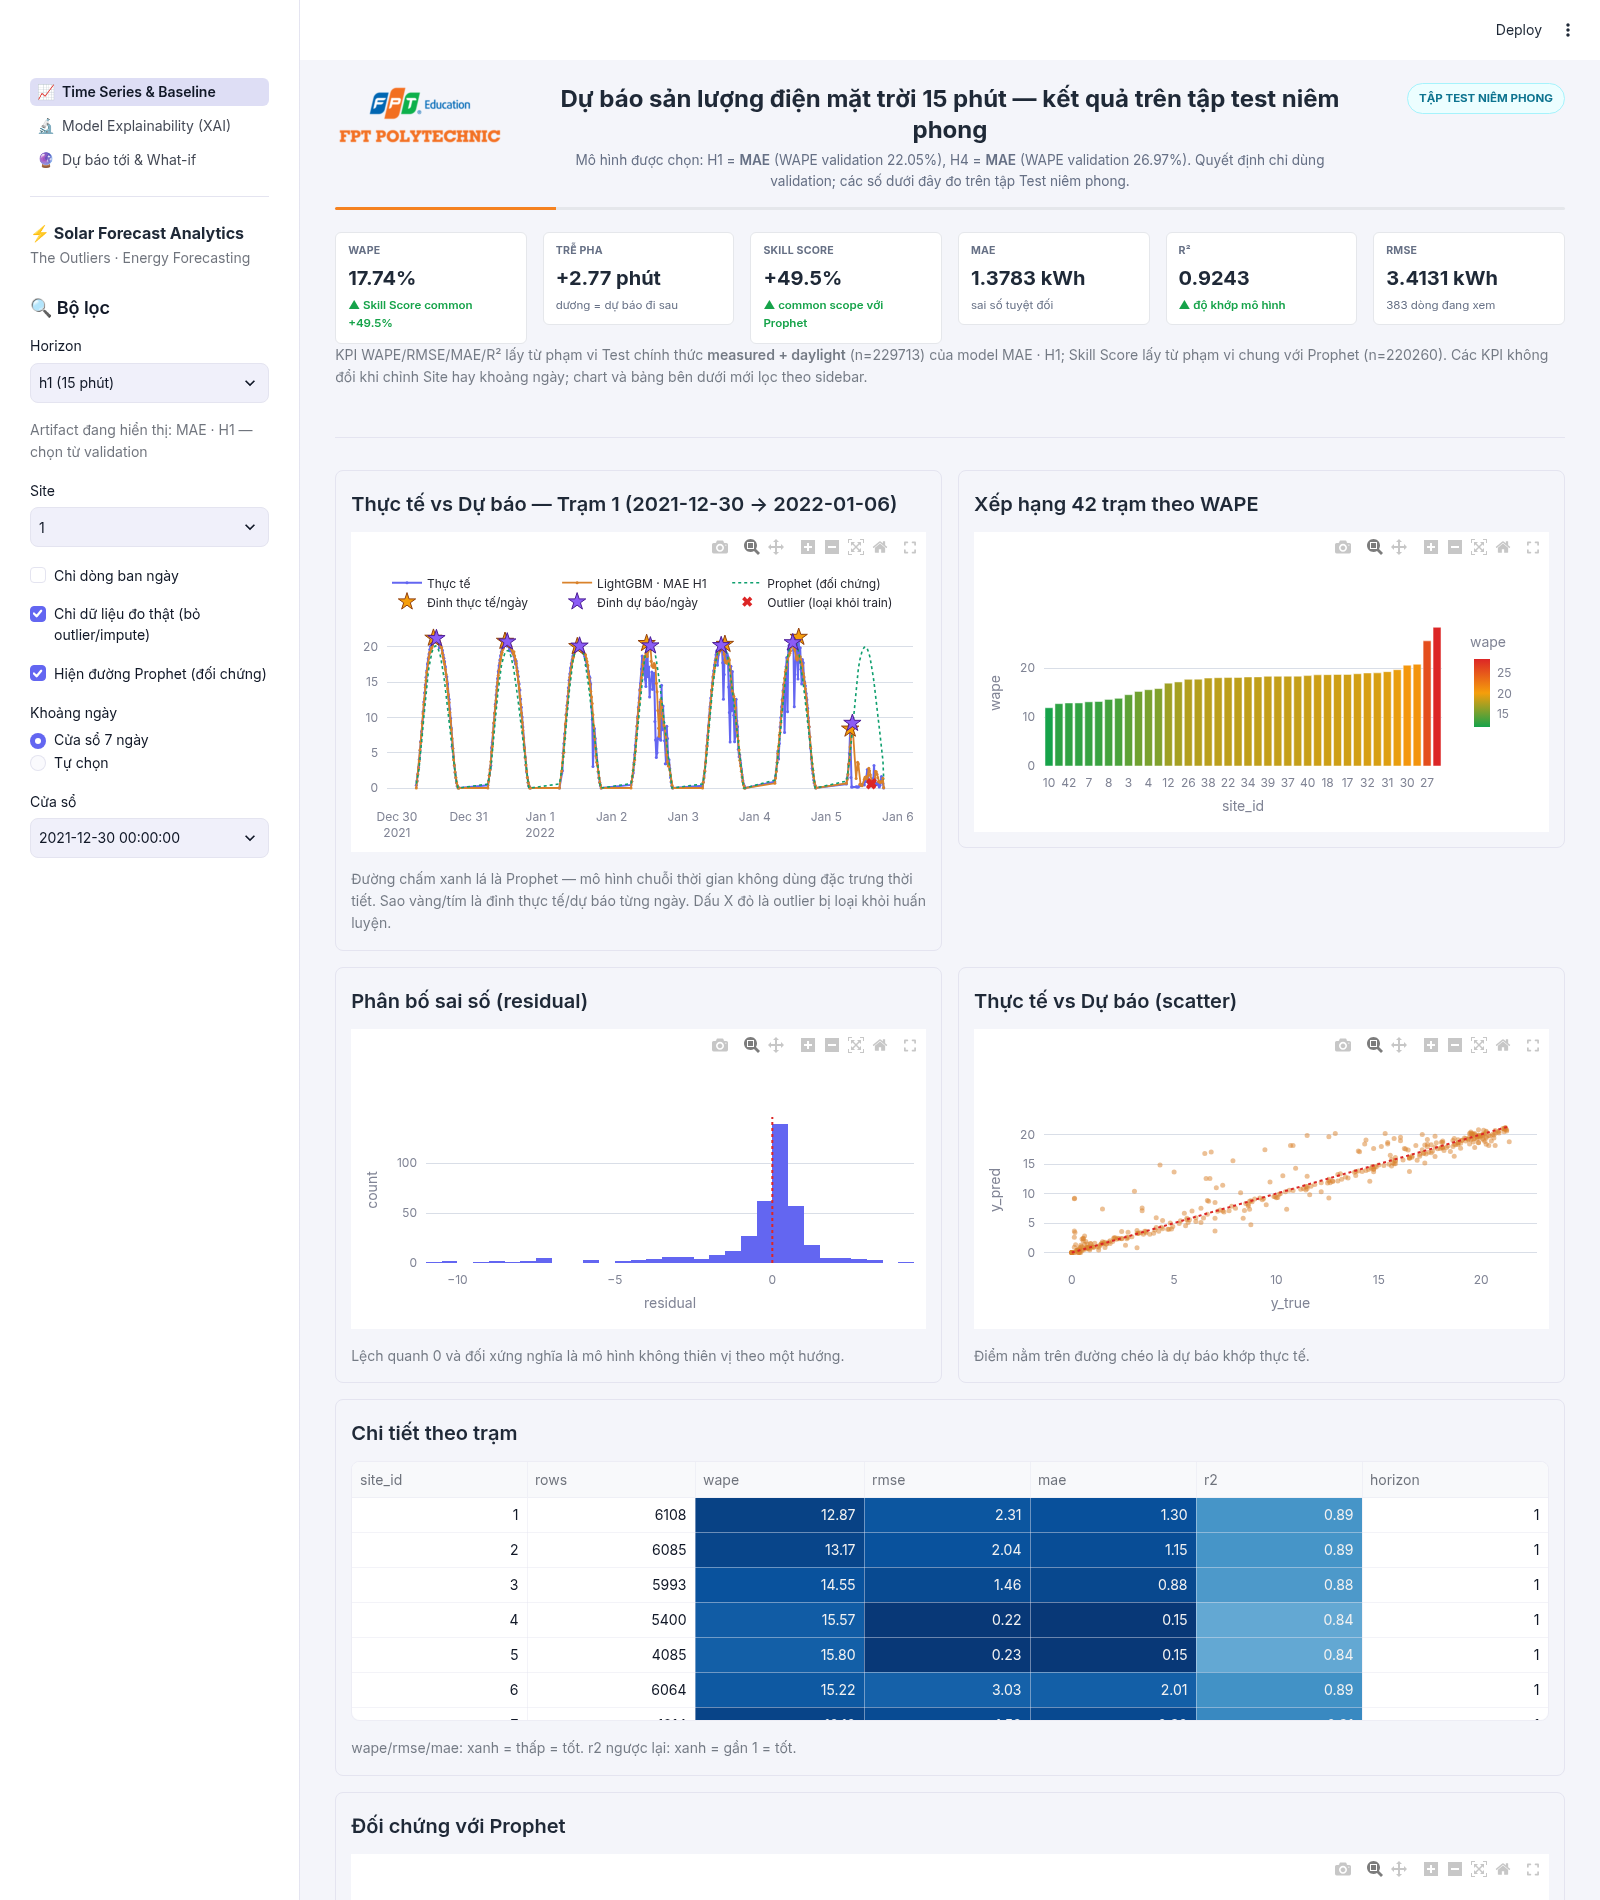
\includegraphics[width=0.82\textwidth]{images/streamlit_1_timeseries.png}
    \caption{Hình 9.3 (Giao diện thực tế từ Streamlit App): Trang Dashboard 1 — Giám sát Chuỗi thời gian Sản lượng Thực tế và Dự báo ($h=1$)}
    \label{fig:st_page1}
\end{figure}

\subsubsection{Phân Tích Chuyên Sâu Thanh Bộ Lọc Sidebar (Sidebar Control Panel)}
Thanh bộ lọc Sidebar tại Trang 1 cung cấp khả năng điều khiển ma trận dữ liệu đầu vào cho toàn bộ các biểu đồ bên dưới:
\begin{itemize}
    \item \textbf{Nguồn mô hình (Model Source):} Cho phép chuyển đổi giữa các phiên bản mô hình khác nhau: \texttt{06\_1 - MAE loss (khu tre pha)}, \texttt{06\_2 - Huber loss}, \texttt{06\_3 - MSE loss}, và \texttt{07 final test}.
    \item \textbf{Tầm dự báo (Horizon):} Selectbox cho phép chuyển đổi giữa bước dự báo ngắn $h=1$ (15 phút) và $h=4$ (60 phút).
    \item \textbf{Lọc theo Từng Trạm Pin (Site Selector):} Cho phép kỹ sư chọn riêng từng trạm trong ma trận 42 trạm (từ Site 1 đến Site 42, mặc định hiển thị Site 19).
    \item \textbf{Bộ lọc Thời gian Ban ngày (Daylight Rows Only):} Lọc chỉ giữ lại các dòng dữ liệu ban ngày ($is\_daylight = True$).
    \item \textbf{Bộ lọc Dữ liệu Đo Thật (Measured Only):} Lọc loại bỏ các dòng bị gán nhãn bất thường ($physical\_over\_capacity$) hoặc dữ liệu phẳng do mất tín hiệu cảm biến ($etl\_imputed$).
    \item \textbf{Chế độ khung thời gian (Date Mode):} Hỗ trợ chọn cửa sổ kiểm tra bảy ngày hoặc khoảng thời gian do người dùng xác định.
\end{itemize}

\subsubsection{Hệ thống 6 Thẻ KPI Executive Metric Cards (Tầng 1)}
Tầng 1 hiển thị 6 thẻ chỉ số được tính toán trên toàn bộ tập test của mô hình đang chọn:
\begin{enumerate}
    \item \textbf{WAPE (\%):} Hiển thị WAPE của mô hình và mức giảm WAPE tương đối so với baseline Prophet.
    \item \textbf{Độ trễ pha (phút):} Hiển thị ước lượng độ trễ dựa trên độ dốc của đường dự báo và đường thực tế.
    \item \textbf{RMSE (kWh):} Hiển thị căn bậc hai của trung bình bình phương sai số.
    \item \textbf{MAE (kWh):} Hiển thị trung bình sai số tuyệt đối.
    \item \textbf{Hệ số $R^2$:} Hiển thị mức độ giải thích biến thiên của dữ liệu theo định nghĩa của chỉ số $R^2$.
    \item \textbf{Số lượng Mẫu (N):} Số lượng dòng quan sát thực tế trong tập test đang xét.
\end{enumerate}

\subsubsection{Chart 1.1 — Biểu đồ Chuỗi thời gian Phân tích Chi tiết Theo Từng Site (Time Series Detail)}
\begin{itemize}
    \item \textbf{Vị trí giao diện:} Khu vực trung tâm chính ban đầu (Hình \ref{fig:st_page1}).
    \item \textbf{Thành phần trực quan:}  
    \begin{itemize}
        \item \textbf{Đường Thực tế (Xanh Indigo \texttt{\#6366F1}):} Chuỗi thời gian sản lượng điện năng $y_{\text{true}}$ (kWh).
        \item \textbf{Đường Dự báo (Cam \texttt{\#D9822B}):} Chuỗi thời gian giá trị dự báo $\hat{y}_{\text{pred}}$ của LightGBM.
        \item \textbf{Đỉnh Năng lượng Hằng ngày (Daily Peak Markers):} Thuật toán tự động quét đỉnh từng ngày và gắn Ngôi sao Vàng (\texttt{\#F59E0B}) tại đỉnh thực tế và Ngôi sao Tím (\texttt{\#8B5F6}) tại đỉnh dự báo.
        \item \textbf{Outlier Marker (Dấu X màu đỏ \texttt{\#D2626}):} Đánh dấu các mốc điểm bị lỗi cảm biến hoặc vượt trần công suất vật lý.
    \end{itemize}
    \begin{itemize}
\item \textbf{Phân tích Data Science chuyên sâu:}\\ 
\end{itemize}
    Vị trí hai loại đánh dấu hỗ trợ quan sát trực quan thời điểm đỉnh thực tế và dự báo. Nhận định về độ trễ pha cần dựa trên chỉ số định lượng ở Trang 3, không chỉ dựa vào một cửa sổ đồ thị.
\end{itemize}

\begin{figure}[htbp]
    \centering
    \includegraphics[width=0.82\textwidth]{images/dashboard_main_metrics.png}
    \caption{Hình 9.4 (Giao diện thực tế từ Streamlit App): Trang Dashboard 1 — Cuộn xuống xem Phân bố Dư thừa \& Thẻ KPI WAPE Cards}
    \label{fig:st_main_metrics}
\end{figure}

\subsubsection{Chart 1.2 — Biểu đồ Xếp hạng Sai số WAPE theo 42 Trạm (Site Rank Bar Chart)}
\begin{itemize}
    \item \textbf{Vị trí giao diện:} Cuộn xuống góc bên phải khu vực giữa trang.
    \item \textbf{Thành phần hiển thị:} Biểu đồ cột nằm ngang xếp hạng WAPE (\%) tăng dần của toàn bộ 42 trạm, được tô màu gradient chuyển tiếp từ Xanh lá (tốt) sang Đỏ (cần chú ý).
    \item \textbf{Phân tích Data Science chuyên sâu:}\\ 
    Biểu đồ hỗ trợ nhận diện các trạm có sai số cao để phân tích thêm.
\end{itemize}

\subsubsection{Chart 1.3a — Phân bố Dư thừa Residual Histogram (Residual Distribution)}
\begin{itemize}
    \item \textbf{Vị trí giao diện:} Cuộn xuống khu vực Tầng 2b bên trái (Hình \ref{fig:st_main_metrics}).
    \item \textbf{Thành phần hiển thị:} Biểu đồ tần suất residual $e = y_{\text{true}} - \hat{y}_{\text{pred}}$ với đường nét đứt đỏ tại mốc 0.
    \item \textbf{Phân tích Data Science chuyên sâu:}\\ 
    Đồ thị hỗ trợ quan sát phân bố phần dư quanh mốc 0 và nhận diện khả năng tồn tại chệch hệ thống.
\end{itemize}

\subsubsection{Chart 1.3b — Actual vs Prediction Scatter Plot (Correlation Scatter)}
\begin{itemize}
    \item \textbf{Vị trí giao diện:} Cuộn xuống khu vực Tầng 2b bên phải (Hình \ref{fig:st_main_metrics}).
    \item \textbf{Thành phần hiển thị:} Đồ thị phân tán Scatter Plot giữa giá trị thực tế và dự báo, đính kèm đường chéo chuẩn $y=x$.
    \item \textbf{Phân tích Data Science chuyên sâu:}\\ 
    Mức độ tập trung của các điểm quanh đường chéo cho biết mức tương quan giữa giá trị thực tế và giá trị dự báo.
\end{itemize}

\subsubsection{Chart 1.4 — Bảng Chi Tiết Theo Site với Conditional Formatting (Site Metrics Table)}
\begin{itemize}
    \item \textbf{Vị trí giao diện:} Khu vực bảng biểu Tầng 3.
    \item \textbf{Thành phần hiển thị:} Bảng dữ liệu thống kê chi tiết từng site (WAPE, RMSE, MAE, $R^2$, N) được áp dụng tô nền màu tự động dải màu Blues.
    \item \textbf{Phân tích Data Science chuyên sâu:}\\ 
    Cho phép tra cứu định lượng chính xác hiệu năng của từng trạm pin.
\end{itemize}

\subsubsection{Chart 1.5 — Biểu đồ Đối sánh WAPE với Prophet Baseline (Baseline Comparison)}
\begin{itemize}
    \item \textbf{Vị trí giao diện:} Khung biểu đồ cuối Trang 1.
    \item \textbf{Thành phần hiển thị:} Biểu đồ thanh nằm ngang đối sánh chỉ số WAPE giữa LightGBM MAE (17,9530\%) và mô hình đối chứng Prophet (36,3380\%) tại H1, kèm nhãn Skill Score $+50{,}5944\%$ trên 220.114 dòng cùng phạm vi. Đây là benchmark Prophet, không phải persistence.
    \item \textbf{Phân tích Data Science chuyên sâu:}\\ 
    Biểu đồ cung cấp đối sánh trực quan WAPE giữa LightGBM và Prophet trong cùng điều kiện đánh giá.
\end{itemize}

% =============================================================
\begin{figure}[htbp]
    \centering
    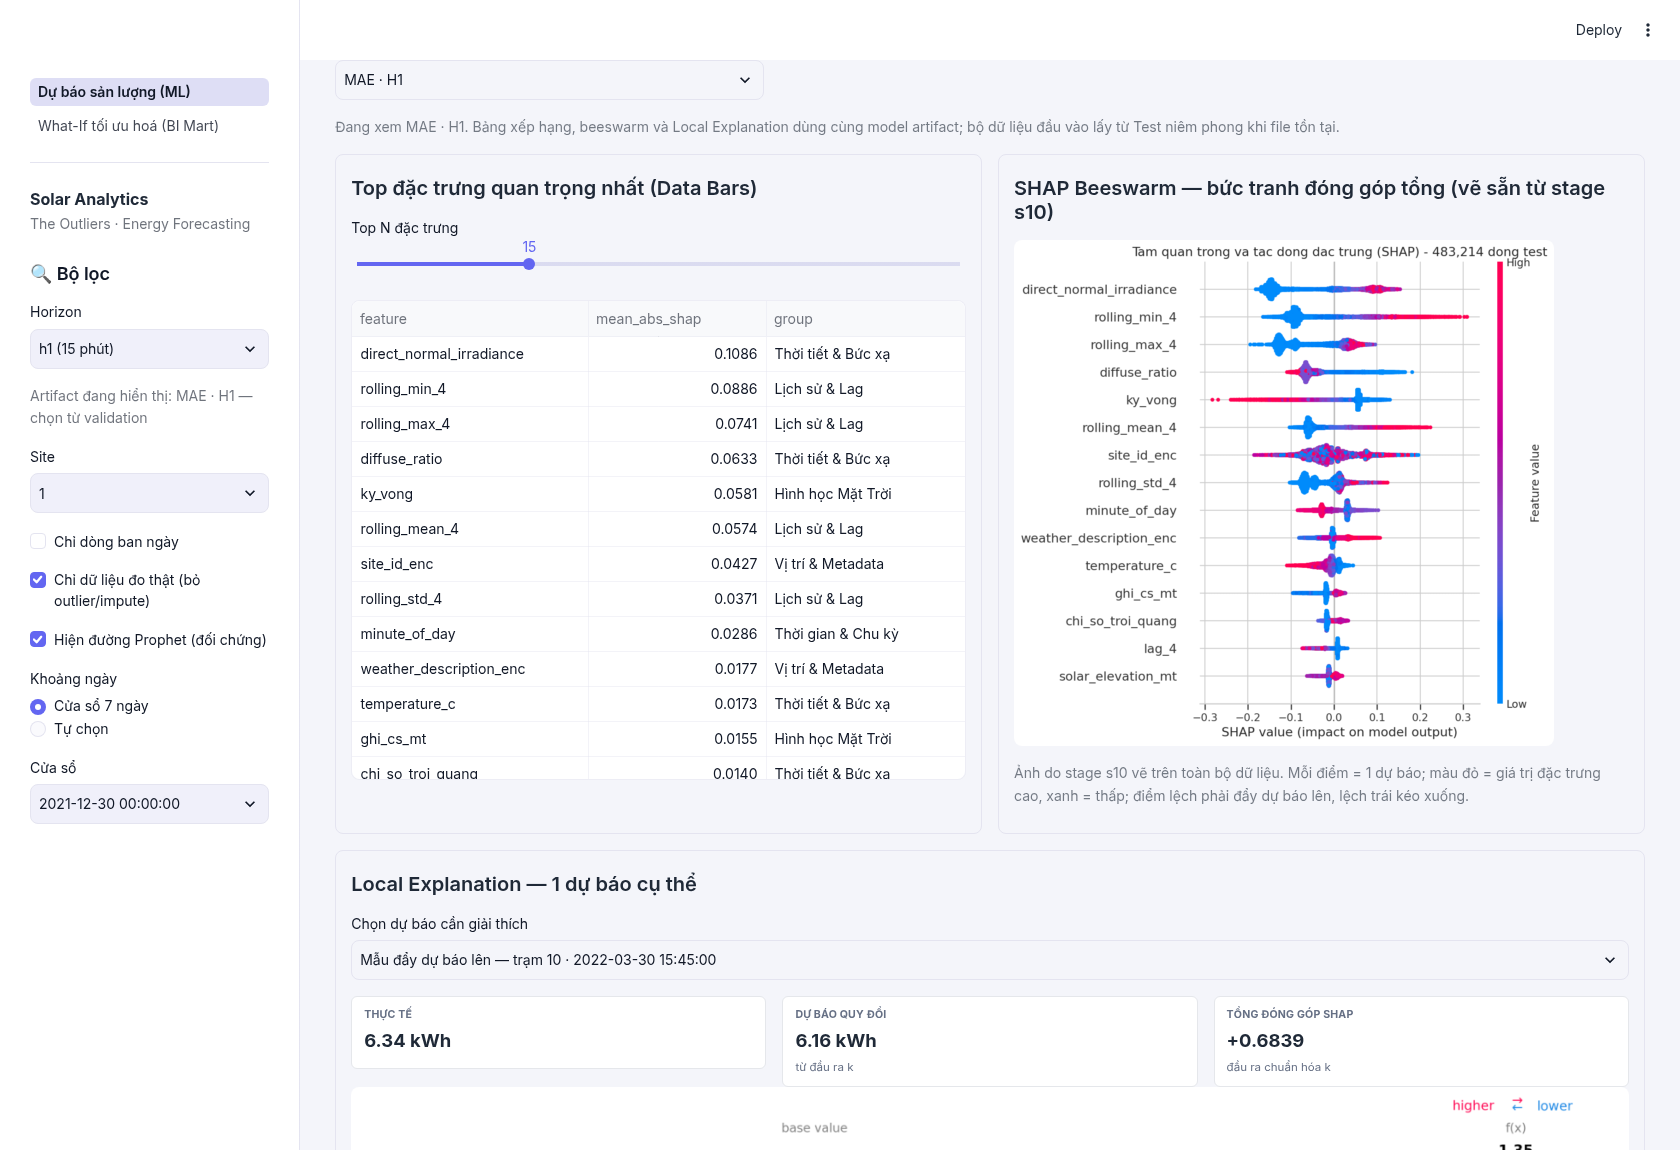
\includegraphics[width=0.82\textwidth]{images/streamlit_2_shap.png}
    \caption{Hình 9.5 (Giao diện thực tế từ Streamlit App): Trang Dashboard 2 — Phân tích Giải thích AI bằng SHAP Beeswarm \& Waterfall}
    \label{fig:st_page2}
\end{figure}

\subsection[Trang 2: Giải Thích AI Bằng SHAP]{Trang Dashboard 2: Phân Tích Minh Bạch AI Bằng SHAP (\texttt{2\_SHAP.py})}

\begin{center}
\fbox{
\begin{minipage}{0.95\linewidth}
\textbf{Vai trò của Trang 2:}
Trang 2 trình bày các giá trị SHAP để giải thích đóng góp của từng đặc trưng đối với dự báo của LightGBM, ở cả mức toàn cục và cục bộ.
\end{minipage}
}
\end{center}

\begin{figure}[htbp]
    \centering
    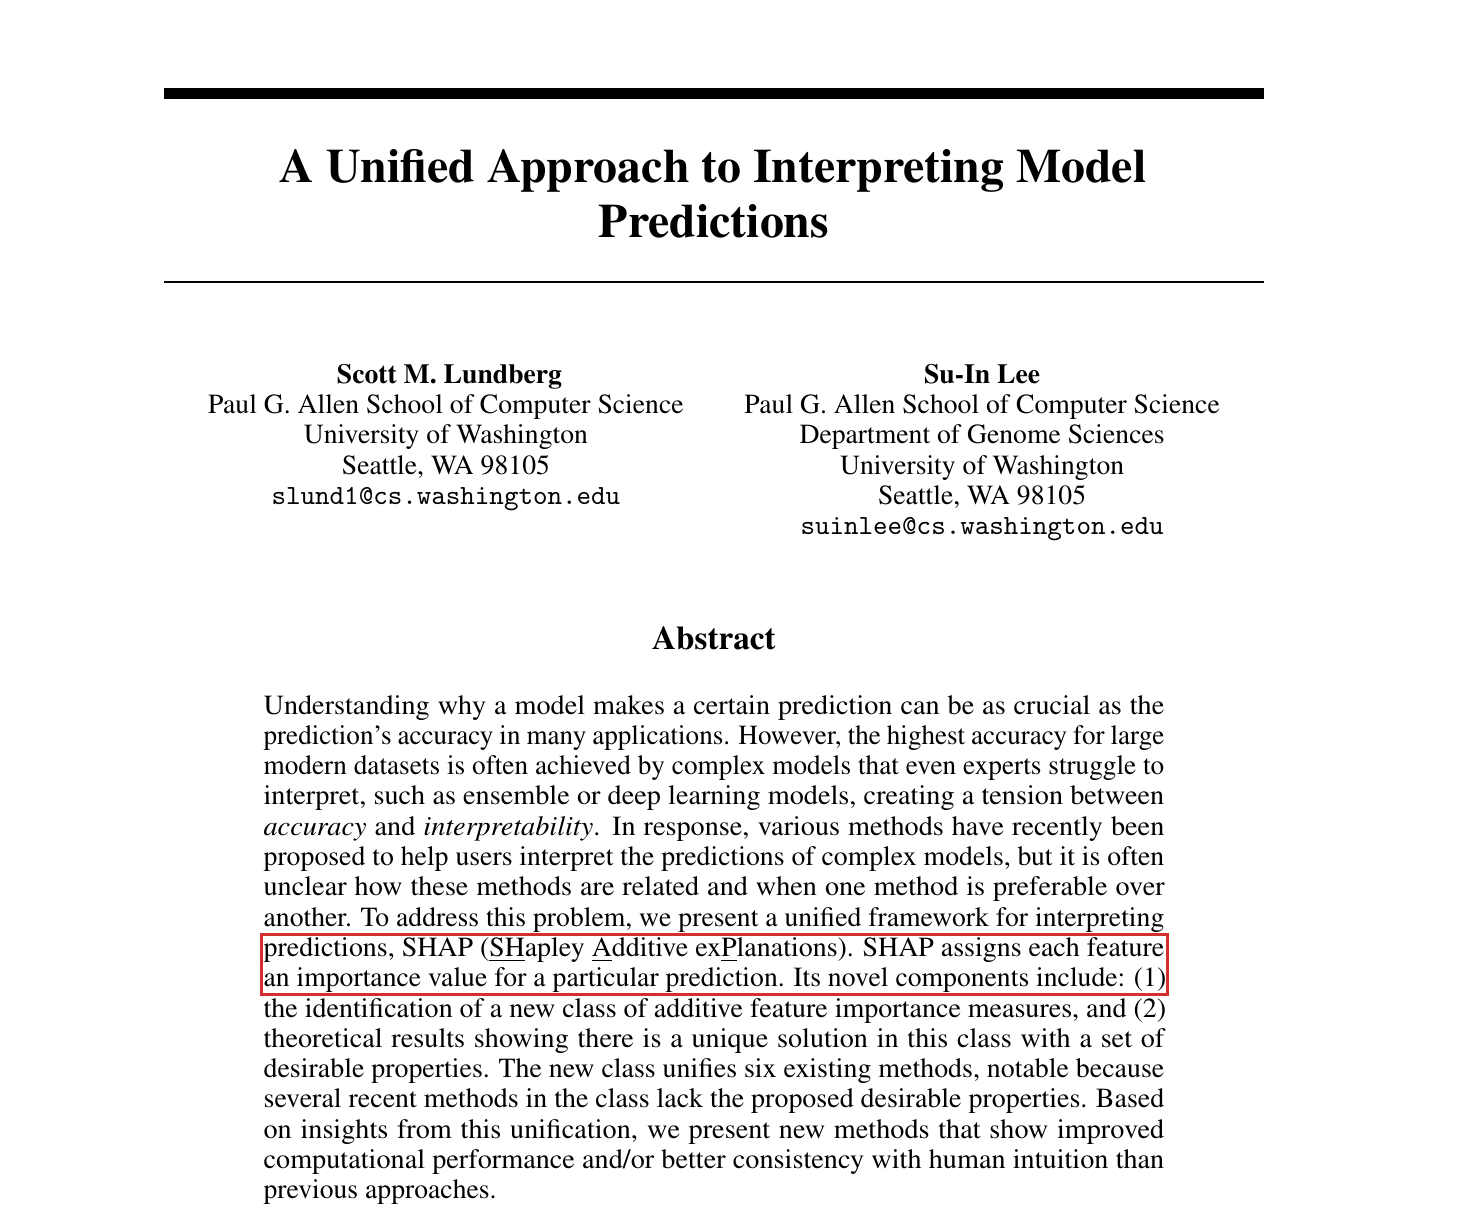
\includegraphics[width=0.88\textwidth]{images/paper_lundberg_shap_2017.png}
    \caption{Ảnh chụp trang đầu của bài báo Lundberg \& Lee (2017)~\cite{lundberg2017}, NeurIPS 30. Abstract giới thiệu SHAP như một khung thống nhất gán giá trị đóng góp cho từng feature tại một dự báo. Dự án áp dụng đúng ngữ cảnh giải thích dự báo đó cho LightGBM; các biểu đồ SHAP bên dưới được tính lại từ mô hình và dữ liệu dự án.}
    \label{fig:paper_shap}
\end{figure}

\subsubsection{Phân Tích Chuyên Sâu Thanh Bộ Lọc XAI Sidebar}
Thanh Sidebar Trang 2 trang bị bộ lọc \textbf{Bộ đặc trưng mô hình (Feature Set Choice)}:
\begin{itemize}
    \item \textbf{Mô hình / horizon:} Dashboard dò các artifact MAE, Huber và MSE cho hai horizon H1/H4, sau đó cho phép chọn động mô hình cần giải thích.
    \item \textbf{Mô hình mặc định:} Khi mở trang, dashboard ưu tiên model thắng được ghi trong \texttt{07\_final\_test/best\_loss.json}; bộ artifact v3 được dùng cho báo cáo ghi MAE cho cả H1 và H4.
\end{itemize}

\subsubsection{Hệ thống Thẻ KPI XAI (Tầng 1)}
\textbf{Trạng thái artifact cần công bố:} Dashboard hỗ trợ chọn động loss/horizon. Các hình SHAP minh họa trong báo cáo phải được đọc cùng tên model và horizon hiển thị trong hình; không mặc định coi mọi hình cũ là kết quả của Huber. Tổng SHAP vẫn ở thang đầu ra chuẩn hóa $k$, còn KPI dự báo được quy đổi về kWh theo công thức của pipeline.
Hiển thị 3 thẻ tổng quan: ``Số đặc trưng'' ($54$, đếm trực tiếp số dòng của \texttt{08\_explain/shap\_importance.csv}), ``Đặc trưng quan trọng nhất'' (đặc trưng có $\overline{|SHAP|}$ lớn nhất), và ``Nhóm đóng góp nhiều nhất'' (nhóm có tổng $|SHAP|$ lớn nhất).

\subsubsection{Chart 2.1 — Biểu đồ Tròn Tỷ Trọng Đóng Góp Nhóm Đặc Trưng (Group Importance Pie Chart)}
\begin{itemize}
    \item \textbf{Vị trí giao diện:} Tầng 2 bên phải (Hình \ref{fig:st_page2}).
    \item \textbf{Thành phần hiển thị:} Biểu đồ bánh doughnut thể hiện tỷ lệ tổng $|SHAP|$ giữa các nhóm hiện tại: Vị trí và metadata ($37{,}98\%$), Lịch sử và lag ($28{,}32\%$), Thời gian và chu kỳ ($23{,}46\%$), Thời tiết và bức xạ ($10{,}23\%$).
    \item \textbf{Phân tích Data Science chuyên sâu:}\\ 
    Biểu đồ cho biết tỷ trọng đóng góp của các nhóm đặc trưng theo tổng giá trị tuyệt đối SHAP trong mẫu phân tích.
\end{itemize}

\subsubsection{Chart 2.2 — Bảng Xếp Hạng Data Bars Top Đặc Trưng (Global Importance Table)}
\begin{itemize}
    \item \textbf{Vị trí giao diện:} Tầng 2 bên trái.
    \item \textbf{Thành phần hiển thị:} Bảng xếp hạng Top N đặc trưng theo giá trị $\text{mean}(|\text{SHAP}|)$ đính kèm thanh Data Bars màu tím Indigo\\(\texttt{st.dataframe(\_styler)}).
    \item \textbf{Phân tích Data Science chuyên sâu:}\\ 
    Bảng cho phép xác định các đặc trưng có giá trị SHAP trung bình lớn trong mẫu phân tích.
\end{itemize}

\subsubsection{Chart 2.3 — Cột Nằm Ngang LightGBM Native Gain Importance (Native Gain Bar Chart)}
\begin{itemize}
    \item \textbf{Vị trí giao diện:} Khung bên trái hàng A (Global Explanation).
    \item \textbf{Thành phần hiển thị:} Biểu đồ cột nằm ngang xếp hạng đặc trưng dựa trên chỉ số Gain trung bình cộng dồn qua tất cả các cây quyết định trong mô hình LightGBM.
    \item \textbf{Phân tích Data Science chuyên sâu:}\\ 
    Biểu đồ được dùng để đối chiếu thứ hạng theo Gain với kết quả giải thích theo SHAP.
\end{itemize}

\subsubsection[Chart 2.4 — SHAP Dependence Plot]{Chart 2.4 — SHAP Dependence Plot Phi Tuyến\\(\texttt{shap.plots.scatter})}
\begin{itemize}
    \item \textbf{Vị trí giao diện:} Khung bên phải hàng A (Hình \ref{fig:st_split_subplots}).
    \item \textbf{Thành phần hiển thị:} Đồ thị phân tán SHAP Dependence Plot được vẽ bằng \texttt{shap.plots.scatter}, cho phép lựa chọn biến để xem quan hệ phi tuyến.
    \item \textbf{Phân tích Data Science chuyên sâu:}\\ 
    Trục hoành hiển thị giá trị thực tế của bức xạ ($0 - 1100\text{ W/m}^2$), trục tung hiển thị biên độ tác động SHAP. Đồ thị cho thấy rõ ngưỡng phi tuyến tại mốc bức xạ $400\text{ W/m}^2$, khi vượt qua ngưỡng này, SHAP value chuyển từ âm (làm giảm) sang dương (làm tăng sản lượng).
\end{itemize}

\begin{figure}[htbp]
    \centering
    \includegraphics[width=0.82\textwidth]{images/dashboard_split_subplots.png}
    \caption{Hình 9.6 (Giao diện thực tế từ Streamlit App): Trang Dashboard 2 — Cuộn xuống xem Subplots SHAP Dependence Plot}
    \label{fig:st_split_subplots}
\end{figure}

\subsubsection{Chart 2.5 — Local Explanation Phân Tích Chi Tiết 1 Dự Báo Cụ Thể (\texttt{shap.plots.\allowbreak force})}
\begin{itemize}
    \item \textbf{Vị trí giao diện:} Hàng B toàn chiều rộng (Full-width Container, Hình \ref{fig:st_local_force}).
    \item \textbf{Thành phần hiển thị:} Người dùng chọn một dòng bất kỳ theo cặp \texttt{site\_id + timestamp} tại bộ chọn cuối trang. Biểu đồ Force Plot (\texttt{shap.plots.\allowbreak force}) giải thích riêng dự báo của dòng đang chọn.
    \item \textbf{Mẫu minh họa trên Hình \ref{fig:st_local_force}:} Dòng được chọn là Site 30 tại \texttt{2022-02-24 12:30:00}, sản lượng thực hiển thị $3{,}17$ kWh. Dashboard ghi tổng đóng góp SHAP là $-0{,}2972$ so với giá trị nền; các mũi tên màu xanh kéo dự báo xuống, nổi bật ở \texttt{direct\_normal\_irradiance}, \texttt{ky\_vong}, \texttt{rolling\_min\_4}, \texttt{rolling\_mean\_4}, \texttt{diffuse\_ratio} và \texttt{weather\_condition\_enc}; mũi tên đỏ kéo dự báo lên. Giá trị nền hiện được lấy trực tiếp từ \texttt{TreeExplainer} của mô hình đang chọn, không lấy trung bình tổng SHAP của mẫu.
    \item \textbf{Chọn mô hình động:} Bộ lọc XAI dò các artifact \texttt{MAE/H1}, \texttt{MAE/H4}, \texttt{Huber/H1}, \texttt{Huber/H4}, \texttt{MSE/H1} và \texttt{MSE/H4}. Gain, SHAP, local explanation và What-if dùng cùng loss/horizon; nếu chưa có file SHAP lưu sẵn, dashboard tính một mẫu SHAP xác định gồm tối đa $2.000$ dòng từ artifact được chọn.
    \item \textbf{Ba mẫu local từ Notebook:} Notebook chọn ba dòng từ $2.000$ dòng SHAP theo ba trạng thái: đóng góp tổng lớn nhất, nhỏ nhất và gần baseline nhất. Dashboard hiển thị nhanh ba mẫu này nhưng vẫn giữ bộ chọn thủ công theo \texttt{site\_id + timestamp}. Tổng SHAP, phần dương và phần âm là trên đầu ra đã chuẩn hóa của MAE H1, không phải kWh; sản lượng thực là nhãn đo được sau phép nối theo \texttt{site\_id + timestamp}.
\end{itemize}

\begin{table}[H]
\centering
\small
\caption{Ba mẫu Local SHAP được chọn tự động từ mẫu SHAP của MAE H1. Dự báo quy đổi dùng kWh, còn các thanh đỏ/xanh và tổng SHAP dùng thang chuẩn hóa của mô hình.}
\label{tab:local_shap_business_cases}
\begin{tabularx}{\linewidth}{>{\raggedright\arraybackslash}p{1.35cm} >{\raggedright\arraybackslash}p{2.35cm} r >{\raggedright\arraybackslash}p{2.55cm} >{\raggedright\arraybackslash}X}
\toprule
\textbf{Mẫu} & \textbf{Mốc mẫu} & \textbf{Thực tế / dự báo (kWh)} & \textbf{SHAP tổng; dương/âm} & \textbf{Diễn giải cho khách hàng/vận hành} \\
\midrule
\textbf{A} & Site 10; 12/03/2022 11:15 & $6{,}719 / 6{,}816$ & $+0{,}6072$; $+0{,}6577/-0{,}0505$ & DNI, trần công suất và rolling minimum một giờ cùng kéo lên; dự báo gần thực tế. \\
\textbf{B} & Site 25; 16/03/2022 18:15 & $10{,}063 / 0{,}000$ & $-0{,}7141$; $+0{,}1481/-0{,}8623$ & Tín hiệu cuối ngày kéo xuống mạnh; cần ưu tiên kiểm tra timestamp, bức xạ và inverter. \\
\textbf{C} & Site 39; 26/12/2021 12:15 & $2{,}629 / 4{,}032$ & $+0{,}0006$; $+0{,}2177/-0{,}2171$ & Biến kéo lên và kéo xuống gần triệt tiêu; phù hợp để minh họa bất định, không kết luận lỗi thiết bị. \\
\bottomrule
\end{tabularx}
\end{table}

\textbf{Ý nghĩa nghiệp vụ của hai màu trong Force Plot:} Màu xanh không có nghĩa ``thiết bị xấu'' và màu đỏ không có nghĩa ``thiết bị tốt''; chúng chỉ mô tả hướng đóng góp của các đầu vào đối với dự báo tại một timestamp. Quyết định vận hành phải đối chiếu thêm sản lượng đo, bức xạ, điều kiện mây và trạng thái inverter. Vì vậy, SHAP được dùng như công cụ ưu tiên kiểm tra và giải thích cho khách hàng, không phải một phép chẩn đoán nhân quả tự động.

\begin{figure}[H]
    \centering
    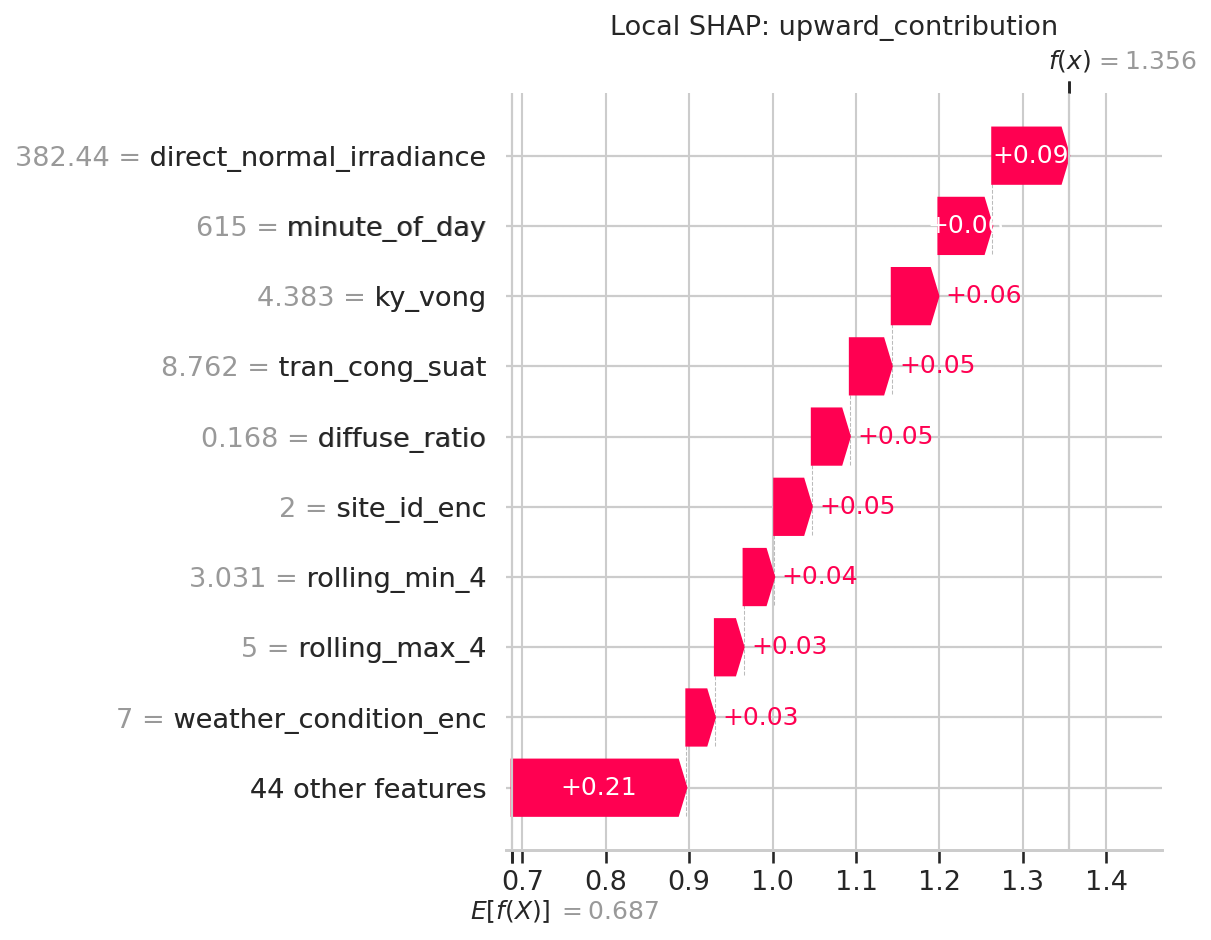
\includegraphics[width=0.86\textwidth]{images/local_shap_mae_h1_upward.png}
    \caption{Local SHAP MAE H1, mẫu A tại Site 10 lúc 11:15. DNI, trần công suất, rolling minimum một giờ và thời điểm trong ngày là các biến đẩy dự báo lên.}
    \label{fig:local_shap_mae_upward}
\end{figure}

\textbf{Ý nghĩa nghiệp vụ của mẫu A:} DNI là tín hiệu vật lý trực tiếp nhất cho sản lượng pin; khi đóng góp dương lớn, hệ thống đang nhận diện điều kiện bức xạ thuận lợi. \texttt{rolling\_min\_4} không phải thời tiết mà là ``sàn'' phát điện của bốn điểm 15 phút gần nhất, giúp vận hành nhận biết hệ thống đang duy trì sản lượng thay vì chỉ có một đỉnh nhất thời. \texttt{tran\_cong\_suat} phản ánh quy mô/trần phát suy ra từ dữ liệu, nên tác động dương không có nghĩa inverter đang phát thêm điện mà cho biết mức công suất hợp lý của trạm.

\begin{figure}[H]
    \centering
    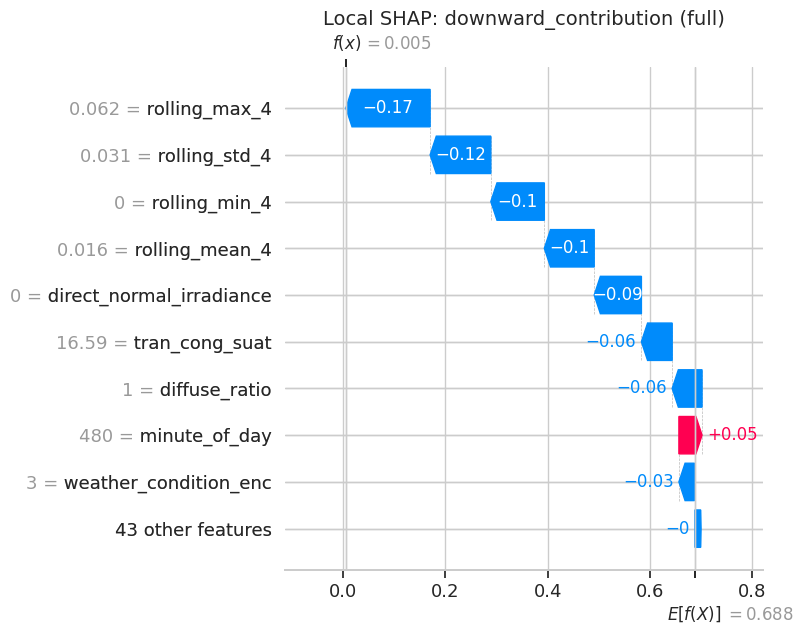
\includegraphics[width=0.86\textwidth]{images/local_shap_mae_h1_downward.png}
    \caption{Local SHAP MAE H1, mẫu B tại Site 25 lúc 18:15. Thời điểm trong ngày, chỉ số bức xạ bầu trời quang và kỳ vọng sản lượng kéo dự báo xuống mạnh.}
    \label{fig:local_shap_mae_downward}
\end{figure}

\textbf{Ý nghĩa nghiệp vụ của mẫu B:} \texttt{minute\_of\_day} và \texttt{interval\_hour} mã hóa vị trí thời gian, còn \texttt{ghi\_cs\_mt} và \texttt{ky\_vong} mô tả mức phát kỳ vọng theo hình học Mặt Trời và quy mô trạm. Vì nhãn đo được tại mốc này vẫn là $10{,}063$ kWh trong khi dự báo quy đổi là $0$ kWh, đây là một ca cần kiểm tra chất lượng dữ liệu và vận hành: đối chiếu múi giờ/mốc ghép, bức xạ cuối ngày, trạng thái inverter và các trạm lân cận. SHAP giải thích vì sao mô hình suy giảm dự báo, nhưng không tự chứng minh nguyên nhân.

\begin{figure}[H]
    \centering
    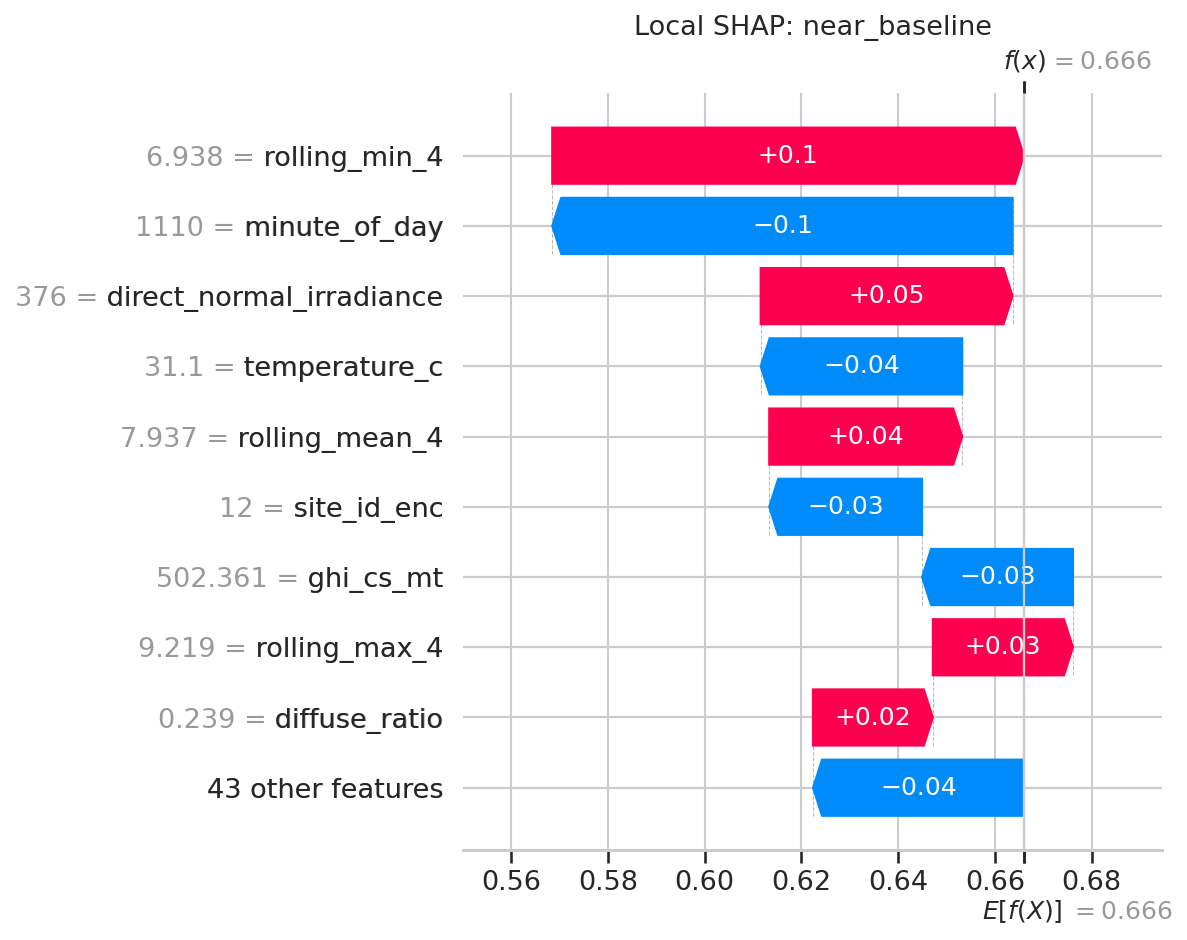
\includegraphics[width=0.86\textwidth]{images/local_shap_mae_h1_baseline.png}
    \caption{Local SHAP MAE H1, mẫu C tại Site 39 lúc 12:15. Các tín hiệu quy mô và lịch sử kéo lên gần như triệt tiêu với DNI, kỳ vọng và mã thời tiết kéo xuống.}
    \label{fig:local_shap_mae_baseline}
\end{figure}

\textbf{Ý nghĩa nghiệp vụ của mẫu C:} Tổng SHAP chỉ $+0{,}0006$ không có nghĩa mọi biến đều không quan trọng; nó cho thấy các lực kéo lên và kéo xuống gần triệt tiêu. Đây là tình huống phù hợp để giải thích cho khách hàng vì có thể chỉ ra cả hai phía của dự báo. Riêng \texttt{weather\_description\_enc} là mã hóa phân loại, do đó dấu SHAP chỉ áp dụng cho trạng thái thời tiết của dòng đang xét, không được diễn giải như một thang điểm ``thời tiết xấu hơn'' theo giá trị số.

\begin{figure}[htbp]
    \centering
    \includegraphics[width=0.82\textwidth]{images/dashboard_page2_local_force.png}
    \caption{Hình 9.7 (Giao diện thực tế từ Streamlit App): Trang Dashboard 2 — Bộ chọn mô hình, ba mẫu local từ Notebook 08 và bộ lọc thủ công theo \texttt{site\_id + timestamp}. Ba hình \ref{fig:local_shap_mae_upward}--\ref{fig:local_shap_mae_baseline} mới là các output số liệu MAE H1 dùng trong phân tích trên.}
    \label{fig:st_local_force}
\end{figure}

% =============================================================
\begin{figure}[htbp]
    \centering
    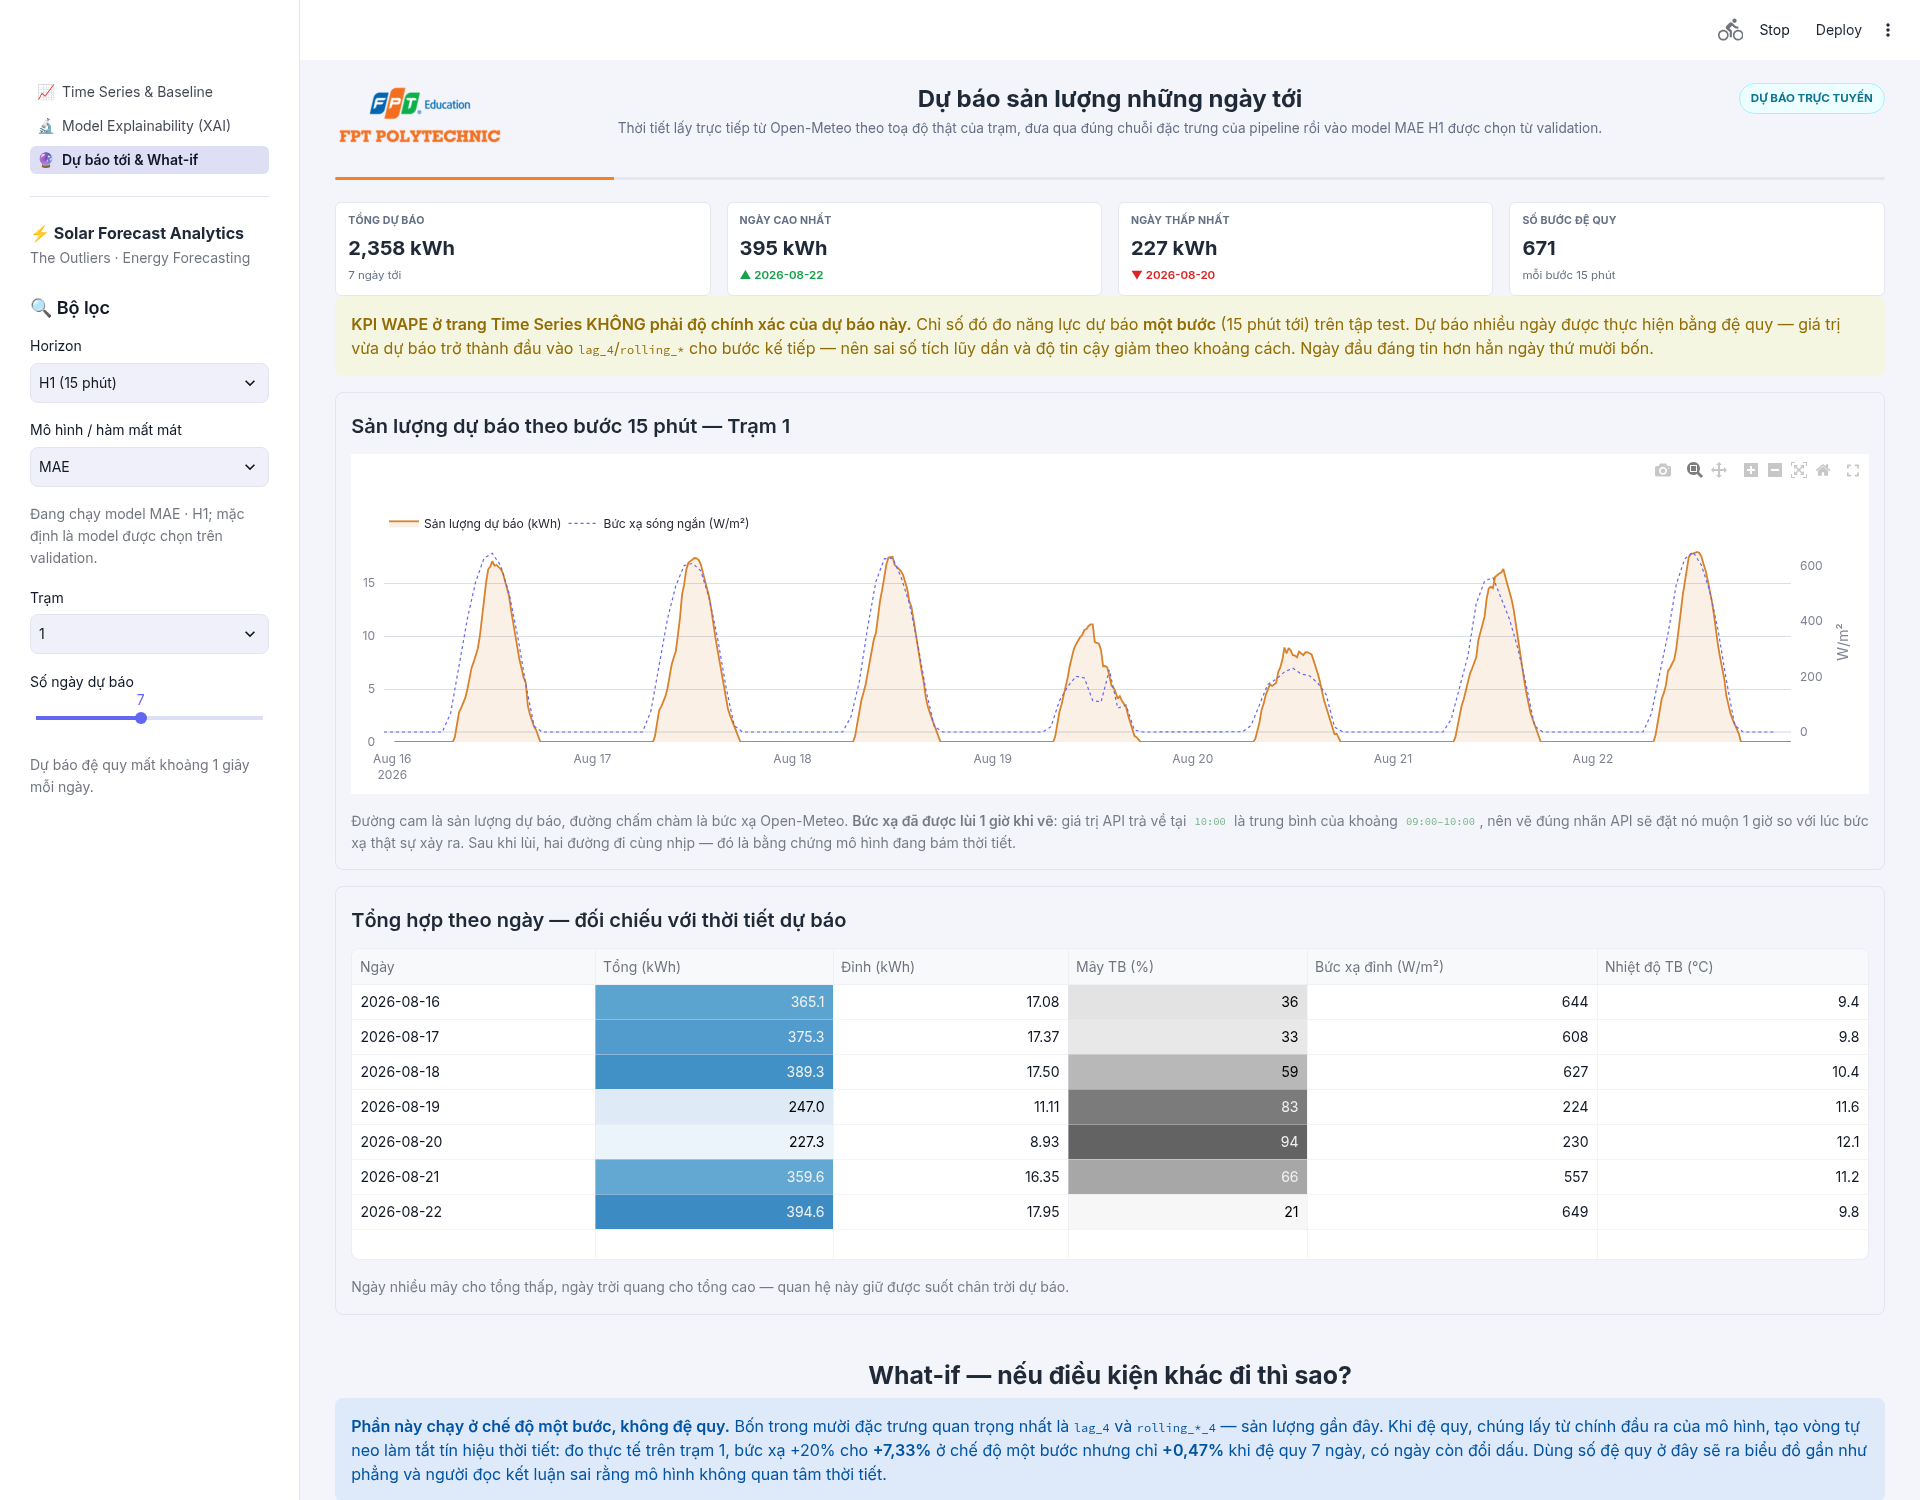
\includegraphics[width=0.82\textwidth]{images/streamlit_3_du_bao.png}
    \caption{Hình 9.9: Giao diện Trang Dashboard 3, gồm giám sát GMM--IF và phân tích độ trễ pha.}
    \label{fig:st_page3}
\end{figure}

\subsection[Trang 3: Dự Báo Tới \& What-if]{Trang Dashboard 3: Dự Báo Những Ngày Tới \& Phân Tích Độ Nhạy (\texttt{3\_Du\_Bao.py})}

\begin{center}
\fbox{
\begin{minipage}{0.95\linewidth}
\textbf{Vai trò của Trang 3:}
Hai trang đầu trình bày hiệu năng \emph{đã đo được} trên tập kiểm thử. Trang 3 tập trung giải quyết một bài toán khác: \emph{dự báo sản lượng trong tương lai}. Trang này gọi trực tiếp API Open-Meteo theo toạ độ thật của trạm, đưa dữ liệu khí tượng qua đúng chuỗi đặc trưng của pipeline rồi vào mô hình tốt nhất.
\end{minipage}
}
\end{center}

Ba trang được tách theo \textbf{bản chất dữ liệu}, không theo chủ đề: trang 1 và 2 đọc kết quả pipeline đã ghi sẵn nên hiển thị tức thời; trang 3 phải gọi mạng và chạy mô hình nên chậm hơn. Việc tách này còn nhằm tránh một hiểu nhầm nghiêm trọng: nếu đặt dự báo mười bốn ngày cạnh chỉ số $\text{WAPE}=17{,}64\%$ ở trang 1, người xem rất dễ đọc con số đó thành độ chính xác của dự báo dài hạn, trong khi nó chỉ đo năng lực dự báo \textbf{một bước} (15 phút).

\subsubsection{Cơ Chế Dự Báo Đệ Quy Cho Chân Trời Dài}
Mô hình được huấn luyện để dự báo một bước. Để mở rộng tầm dự báo, hệ thống áp dụng cơ chế \textbf{đệ quy}: giá trị vừa dự báo được đưa ngược vào lịch sử, trở thành đầu vào của các đặc trưng \texttt{lag\_4} và \texttt{rolling\_*} cho bước kế tiếp. Chân trời mười bốn ngày tương ứng $14 \times 96 = 1344$ bước.

Tập đặc trưng được chia làm hai nhóm với cách xử lý khác nhau:
\begin{itemize}
    \item \textbf{Nhóm biết trước} --- hình học Mặt Trời, nhãn thời gian, khí tượng dự báo --- tính một lần cho toàn bộ chân trời ngay từ đầu, không phụ thuộc sản lượng.
    \item \textbf{Nhóm phụ thuộc sản lượng} --- \texttt{lag\_4}, \texttt{lag\_96}, \texttt{rolling\_*} --- phải tính lại sau mỗi bước từ lịch sử cộng các giá trị vừa dự báo.
\end{itemize}

Sai số vì thế tích luỹ theo khoảng cách: ngày đầu có độ tin cậy cao hơn đáng kể so với ngày thứ mười bốn. Đây là bản chất của dự báo đệ quy, không phải lỗi cài đặt.

\begin{figure}[htbp]
    \centering
    \includegraphics[width=0.95\textwidth]{images/code_forecast_de_quy.png}
    \caption{Vòng lặp đệ quy trong \texttt{DichVuDuBao.du\_bao()}. Hai dòng được đóng khung là mấu chốt: \texttt{lag\_4} lấy từ mảng lịch sử đang lớn dần, và \texttt{y.append(y\_bao)} đưa giá trị vừa dự báo trở lại mảng đó. Mỗi vòng lặp vì thế kế thừa sai số của mọi vòng trước.}
    \label{fig:code_forecast_de_quy}
\end{figure}

\subsubsection{Kiểm Chứng Trực Quan: Sản Lượng Bám Theo Bức Xạ}
Biểu đồ chính vẽ chồng hai đường trên hai trục tung: sản lượng dự báo (kWh) và bức xạ sóng ngắn lấy từ Open-Meteo (W/m\textsuperscript{2}). Hai đường đi cùng nhịp qua toàn bộ chân trời --- đây là kiểm chứng end-to-end trực quan nhất cho thấy chuỗi \emph{API khí tượng $\rightarrow$ đặc trưng $\rightarrow$ mô hình} hoạt động đúng.

Bảng tổng hợp theo ngày đặt sản lượng cạnh độ mây và bức xạ đỉnh, cho thấy quan hệ vật lý được giữ nguyên: ngày nhiều mây cho tổng thấp, ngày trời quang cho tổng cao.

\begin{figure}[htbp]
    \centering
    \includegraphics[width=0.95\textwidth]{images/code_forecast_openmeteo.png}
    \caption{Hàm kéo dữ liệu khí tượng từ Open-Meteo. Bảng \texttt{DOI\_TEN\_THOI\_TIET} ánh xạ tên biến của API sang tên mà pipeline đang dùng --- đặt sai một tên ở đây thì đặc trưng tương ứng sẽ bị bỏ qua và không được tạo ra, mô hình vẫn chạy nhưng thiếu tín hiệu.}
    \label{fig:code_forecast_openmeteo}
\end{figure}

\subsubsection{Phân Tích What-if --- Vì Sao Phải Chạy Ở Chế Độ Một Bước}
Phần What-if cho phép nhân hệ số lên bức xạ, nhiệt độ, độ mây và quy mô hệ thống, rồi so kịch bản với hiện trạng. Hệ số được áp \textbf{trước khi} dựng đặc trưng, nên các đặc trưng dẫn xuất (\texttt{temp\_x\_shortwave}, \texttt{cloud\_x\_shortwave}, chỉ số trời quang) cũng thay đổi theo --- đúng cách một biến động khí tượng thật lan trong mô hình.

Phần này chạy ở chế độ \textbf{một bước, không đệ quy}. Lý do nằm ở cấu trúc đặc trưng: bốn trong mười đặc trưng quan trọng nhất là \texttt{lag\_4} và \texttt{rolling\_*\_4}, tức sản lượng gần đây. Trong chế độ đệ quy, chúng lấy giá trị từ chính đầu ra của mô hình, tạo thành một vòng tự tham chiếu làm triệt tiêu tín hiệu khí tượng. Số đo thực nghiệm trên trạm 1 khi tăng bức xạ $20\%$:

\begin{center}
\begin{tabular}{lc}
\toprule
\textbf{Chế độ đo} & \textbf{Thay đổi sản lượng} \\
\midrule
Một bước (lịch sử thật, không đệ quy) & $+7{,}33\%$ \\
Đệ quy bảy ngày & $+0{,}47\%$ \\
\bottomrule
\end{tabular}
\end{center}

Chênh lệch này cho thấy độ nhạy thật của mô hình với khí tượng là $+7{,}33\%$; con số $+0{,}47\%$ là kết quả bị vòng tự tham chiếu làm tắt, thậm chí đổi dấu ở một số ngày. Nếu dùng số đệ quy cho phần What-if, biểu đồ sẽ gần như phẳng và người đọc sẽ kết luận sai rằng mô hình không phụ thuộc vào khí tượng --- điều này hoàn toàn trái với thực tế.

\begin{figure}[htbp]
    \centering
    \includegraphics[width=0.95\textwidth]{images/code_forecast_mot_buoc.png}
    \caption{Hàm \texttt{du\_bao\_mot\_buoc()} dùng cho phần What-if. Dòng được đóng khung là điểm khác biệt duy nhất so với hàm đệ quy: lịch sử được \emph{giữ cố định} ở giá trị đo thật gần nhất cho mọi hàng, thay vì cập nhật sau từng bước. Nhờ vậy phần chênh lệch quan sát được đến hoàn toàn từ thay đổi khí tượng.}
    \label{fig:code_forecast_mot_buoc}
\end{figure}

\subsubsection{Một Quyết Định Thiết Kế Giao Diện}
Giao diện \textbf{không có} thanh trượt tốc độ gió, dù đây là biến khí tượng quen thuộc. Lý do: \texttt{wind\_speed} không nằm trong 54 đặc trưng của mô hình, nên mọi hệ số nhân áp lên nó đều cho đúng $0{,}00\%$ thay đổi --- điều này đã được kiểm chứng bằng thực nghiệm. Việc bố trí công cụ điều khiển không tạo ra tác động nào có thể gây hiểu nhầm cho người dùng, do đó nó được loại bỏ hoàn toàn thay vì để lại kèm chú thích.

\subsubsection{Giới Hạn Diễn Giải}
Phần What-if là \textbf{phân tích độ nhạy của mô hình}, không phải dự báo khí tượng. Nhân bức xạ lên $1{,}3$ lần không có nghĩa trời sẽ nắng hơn $30\%$; nó trả lời câu hỏi ``nếu bức xạ cao hơn $30\%$ thì mô hình dự báo ra sao''. Tương tự, chỉ số $\text{WAPE}$ công bố ở trang 1 đo năng lực một bước trên tập kiểm thử, không phải độ chính xác của chân trời mười bốn ngày trên trang này.

\section[KẾT LUẬN VÀ HƯỚNG PHÁT TRIỂN]{KẾT LUẬN VÀ HƯỚNG PHÁT TRIỂN\\CỦA DỰ ÁN}
Dự án đã xây dựng và đánh giá hệ thống dự báo sản lượng quang điện với các kết quả chính như sau:
\begin{enumerate}
    \item \textbf{Phát hiện bất thường GMM--IF:} Pipeline kết hợp nhiều quy tắc phát hiện và phân loại quan sát bất thường để hỗ trợ làm sạch dữ liệu và đánh giá mô hình.
    \item \textbf{Dự báo ngắn hạn bằng LightGBM:} Bộ artifact validation chọn MAE theo WAPE ở cả H1 ($21{,}0302\%$) và H4 ($25{,}2243\%$). Trên phạm vi Test ban ngày có số đo thật, MAE đạt WAPE $17{,}8226\%$, MAE $1{,}3399$ kWh, $R^2=0{,}9243$ tại H1 và WAPE $21{,}4538\%$, MAE $1{,}5984$ kWh, $R^2=0{,}8993$ tại H4. Các kiểm tra độ trễ pha là chẩn đoán bổ sung, không được dùng để thay thế WAPE.
    \item \textbf{Dashboard phân tích:} Dashboard cung cấp trực quan hóa chuỗi thời gian, chỉ số sai số, phân tích SHAP và kiểm tra độ trễ pha cho người dùng vận hành.
\end{enumerate}


% =============================================================
\section[TÀI LIỆU THAM KHẢO]{TÀI LIỆU THAM KHẢO\\(BIBLIOGRAPHY \& REFERENCES)}

\begin{thebibliography}{99}
\bibitem{zhang2013nrelmetrics}
J. Zhang, B.-M. Hodge, A. Florita, S. Lu, H. F. Hamann, and V. Banunarayanan,
``Metrics for Evaluating the Accuracy of Solar Power Forecasting,''
\href{https://www.nrel.gov/docs/fy14osti/60142.pdf}{www.nrel.gov/docs/fy14osti/60142.pdf} \\ OSTI Link: \url{https://www.osti.gov/biblio/1114086}

\bibitem{zhang2015metrics}
J. Zhang, A. Florita, B.-M. Hodge, S. Lu, H. F. Hamann, V. Banunarayanan, and A. M. Brockway,
``A suite of metrics for assessing the performance of solar power forecasting,''
\textit{Solar Energy}, vol. 111, pp. 157--175, 2015.
DOI: \url{https://doi.org/10.1016/j.solener.2014.10.016}

\bibitem{temporalneto2025pin}
A. Temporal-Neto, R. Pedruzzi, J. B. Melo Filho, and D. M. Moreira,
``PIN: A new metric to evaluate solar irradiance forecast models,''
\textit{Energy Reports}, vol. 13, pp. 2307--2315, 2025.
DOI: \url{https://doi.org/10.1016/j.egyr.2025.01.076}

\bibitem{iec60904}
International Electrotechnical Commission,
\textit{IEC 60904-3:2019 Photovoltaic Devices---Part 3: Measurement Principles for Terrestrial Photovoltaic (PV) Solar Devices with Reference Spectral Irradiance Data}, 2019.
\url{https://webstore.iec.ch/en/publication/64682}

\bibitem{iec61724}
International Electrotechnical Commission,
\textit{IEC 61724-1:2021 Photovoltaic System Performance---Part 1: Monitoring}, 2021.
\url{https://webstore.iec.ch/en/publication/70170}

\bibitem{haurwitz1945}
B. Haurwitz,
``Insolation in Relation to Cloudiness and Cloud Density,''
\textit{Journal of Meteorology}, vol. 2, no. 3, pp. 154--166, 1945.
\url{https://journals.ametsoc.org/view/journals/atsc/2/3/1520-0469_1945_002_0154_iirtca_2_0_co_2.xml}

\bibitem{bailey2024downscaling}
M. Bailey, D. Nychka, M. Sengupta, J. Yang, and S. Bandyopadhyay,
``Temporal and spatial downscaling for solar radiation,'' arXiv:2405.11046, 2024.
\url{https://arxiv.org/abs/2405.11046}
\\ \textit{Ghi chú:} tiền ấn phẩm arXiv, \textbf{chưa qua bình duyệt} tại thời điểm trích dẫn.

\bibitem{lauret2022clearsky}
P. Lauret, R. Alonso-Suárez, J. Le Gal La Salle, and M. David,
``Solar Forecasts Based on the Clear Sky Index or the Clearness Index: Which Is Better?,''
\textit{Solar}, vol. 2, no. 4, pp. 432--444, 2022.
DOI: \url{https://doi.org/10.3390/solar2040026}

\bibitem{grantham2017synthetic}
A. P. Grantham, P. J. Pudney, L. A. Ward, M. Belusko, and J. W. Boland,
``Generating synthetic five-minute solar irradiance values from hourly observations,''
\textit{Solar Energy}, vol. 147, pp. 209--221, 2017.
DOI: \url{https://doi.org/10.1016/j.solener.2017.03.026}

\bibitem{mcdowell2018subhourly}
T. P. McDowell, S. Letellier-Duchesne, and M. Kummert,
``A New Method for Determining Sub-Hourly Solar Radiation from Hourly Data,''
in \textit{2018 Building Performance Analysis Conference and SimBuild}, Chicago, IL, pp. 518--525, 2018.
\url{https://publications.ibpsa.org/proceedings/simbuild/2018/papers/simbuild2018_C071.pdf}

\bibitem{nrelatb2021pv}
National Renewable Energy Laboratory,
``Annual Technology Baseline 2021: Utility-Scale PV,'' 2021.
\url{https://atb.nrel.gov/electricity/2021/utility-scale_pv}

\bibitem{denholm2013capacity}
P. Denholm,
``Solar Energy and Capacity Value,'' NREL/FS-6A20-57582, National Renewable Energy Laboratory, 2013.
DOI: \url{https://doi.org/10.2172/1094876}


\bibitem{li2025gmmif}
X. Li, G. Du, Y. Li, Z. Ma, L. Liu, M. Jiang, F. Liu, and T. Mu,
``Outlier Detection of Photovoltaic Power Generation System Data Based on GMM-IF Algorithm,''
\textit{IEEE Access}, vol. 13, pp. 108823--108837, 2025.
DOI: \url{https://doi.org/10.1109/ACCESS.2025.3581641}

\bibitem{liu2008if}
F. T. Liu, K. M. Ting, and Z.-H. Zhou,
``Isolation Forest,''
in \textit{Proc. 8th IEEE Int. Conf. Data Mining (ICDM)}, Pisa, Italy, 2008, pp. 413--422.
DOI: \url{https://doi.org/10.1109/ICDM.2008.17}

\bibitem{mucomole2026clearsky}
F. V. Mucomole, . A. S. Silva, and L. L. Magaia,
``Photovoltaic modeling of clear sky index correlations at different surface elevation measurement stations at short-measurement scale,''
\textit{Solar Energy Advances}, vol. 6, art. 100129, 2026.
DOI: \url{https://doi.org/10.1016/j.seja.2026.100129}

\bibitem{kwarikunda2021clearsky}
N. Kwarikunda and Z. Chiguvare,
``Performance Analysis of Clear Sky Global Horizontal Irradiance Models: Simple Models Adapted for Local Conditions,''
\textit{Journal of Renewable Energy}, vol. 2021, art. 4369959, 2021.
DOI: \url{https://doi.org/10.1155/2021/4369959}

\bibitem{long2008qcrad}
C. N. Long and Y. Shi,
``An Automated Quality Assessment and Control Algorithm for Surface Radiation Measurements,''
\textit{The Open Atmospheric Science Journal}, vol. 2, pp. 23--37, 2008.
DOI: \url{https://doi.org/10.2174/1874282300802010023}

\bibitem{mabasa2021clearsky}
B. Mabasa, M. D. Lysko, H. Tazvinga, N. Zwane, and S. J. Moloi,
``The Performance Assessment of Six Global Horizontal Irradiance Clear Sky Models in Six Climatological Regions in South Africa,''
\textit{Energies}, vol. 14, no. 9, art. 2583, 2021.
DOI: \url{https://doi.org/10.3390/en14092583}

\bibitem{engerer2014kpv}
N. A. Engerer and F. P. Mills,
``KPV: A clear-sky index for photovoltaics,''
\textit{Solar Energy}, vol. 105, pp. 679--693, 2014.
DOI: \url{https://doi.org/10.1016/j.solener.2014.04.019}

\bibitem{antonanzas2016review}
J. Antonanzas et al.,
``Review of photovoltaic power forecasting,''
\textit{Solar Energy}, vol. 136, pp. 78--111, 2016.
DOI: \url{https://doi.org/10.1016/j.solener.2016.06.069}

\bibitem{lundberg2017}
S. M. Lundberg and S.-I. Lee, 
``A Unified Approach to Interpreting Model Predictions,'' 
in \textit{Advances in Neural Information Processing Systems (NeurIPS 2017)}, vol. 30, pp. 4765--4774, 2017.
\url{https://proceedings.neurips.cc/paper/2017/hash/8a20a8621978632d76c43dfd28b67767-Abstract.html}

\bibitem{ke2017}
G. Ke, Q. Meng, T. Finley, T. Wang, W. Chen, W. Ma, Q. Ye, and T. Y. Liu, 
``LightGBM: A Highly Efficient Gradient Boosting Decision Tree,'' 
in \textit{Advances in Neural Information Processing Systems (NeurIPS 2017)}, vol. 30, pp. 3146--3154, 2017.
\url{https://proceedings.neurips.cc/paper/2017/hash/6449f44a102fde848669bdd9eb6b76fa-Abstract.html}

\bibitem{pvlib2023}
K. S. Anderson, . W. Hansen, W. F. Holmgren, A. R. Jensen, M. A. Mikofski, and A. Driesse,
``pvlib python: 2023 project update,''
\textit{Journal of Open Source Software}, vol. 8, no. 92, pp. 5994, 2023.
DOI: \url{https://doi.org/10.21105/joss.05994}

\bibitem{optuna2019}
T. Akiba, S. Sano, T. Yanase, T. Ohta, and M. Koyama, 
``Optuna: A Next-generation Hyperparameter Optimization Framework,'' 
in \textit{Proc. ACM SIGKDD Int. Conf. Knowledge Discovery \& Data Mining (KDD 2019)}, pp. 2623--2631, 2019.
DOI: \url{https://doi.org/10.1145/3292500.3330701}

\bibitem{leguen2019}
V. Le Guen and N. Thome,
``Shape and Time Distortion Loss for Training Deep Time Series Forecasting Models (DILATE),''
in \textit{Advances in Neural Information Processing Systems (NeurIPS 2019)}, vol. 32, pp. 4191--4203, 2019.
\url{https://arxiv.org/abs/1909.09020}

\bibitem{zou2005elasticnet}
H. Zou and T. Hastie,
``Regularization and Variable Selection via the Elastic Net,''
\textit{Journal of the Royal Statistical Society: Series B}, vol. 67, no. 2, pp. 301--320, 2005.
DOI: \url{https://doi.org/10.1111/j.1467-9868.2005.00503.x}

\bibitem{taylor2018prophet}
S. J. Taylor and B. Letham,
``Forecasting at Scale,''
\textit{The American Statistician}, vol. 72, no. 1, pp. 37--45, 2018.
DOI: \url{https://doi.org/10.1080/00031305.2017.1380080}
\\ \textit{Ghi chú:} bản tiền ấn phẩm PeerJ Preprints 3190v2 (2017) thường được trích dẫn thay cho bản này; tiền ấn phẩm \textbf{chưa qua bình duyệt}, nên nghiên cứu này trích bản đã đăng trên \textit{The American Statistician}.

\bibitem{noaasolarcalculator}
NOAA Global Monitoring Laboratory,
``NOAA Solar Calculator.''
\url{https://gml.noaa.gov/grad/solcalc/}
\end{thebibliography}


\end{document}
